% !TeX spellcheck = <none>
\documentclass[12pt]{report}
%\usepackage[a4paper]{geometry}
\usepackage[right=2.0cm, left=3.5cm, top=2.5cm, bottom=2.5cm]{geometry}
\usepackage[utf8]{inputenc}
%\usepackage{slovak}
\usepackage[slovak]{babel}
\usepackage{epsfig}
\usepackage{color}
\usepackage{url}
\usepackage{amsmath}
\usepackage{amsfonts}
\usepackage{amssymb}
\usepackage{mathtools}
\usepackage{listings}
\usepackage{algpseudocode}
\usepackage{algorithm}
\usepackage{program}
\usepackage{multicol}
\usepackage{framed}
\usepackage{titlesec}
\usepackage{subfig}
\usepackage{textcomp}
\usepackage[mathcal]{euscript}
\usepackage{rotating}
\usepackage{setspace}
\usepackage[table,xcdraw]{xcolor}
\usepackage[sharp,50]{easylist}
\usepackage{enumitem}
\usepackage{courier}
\usepackage{xcolor}
\usepackage{inconsolata}
\usepackage{caption}
\usepackage{pdfpages}
\definecolor{bg}{rgb}{0.95,0.95,0.95}

\renewcommand{\lstlistingname}{Výpis}

\lstdefinelanguage{JavaScript}{
	keywords={typeof, new, true, false, catch, function, return, null, catch, switch, var, if, in, while, do, else, case, break},
	keywordstyle=\color{blue},
	ndkeywords={class, export, boolean, throw, implements, import, this},
	ndkeywordstyle=\color{darkgray}\bfseries,
	identifierstyle=\color{black},
	sensitive=false,
	comment=[l]{//},
	morecomment=[s]{/*}{*/},
	commentstyle=\color{purple}\ttfamily,
	stringstyle=\color{red}\ttfamily,
	morestring=[b]',
	morestring=[b]"
}

\definecolor{gray}{rgb}{0.4,0.4,0.4}
\definecolor{darkblue}{rgb}{0.0,0.0,0.6}
\definecolor{cyan}{rgb}{0.0,0.6,0.6}

\ListProperties(Indent=1em)

\lstset{
  basicstyle=\ttfamily,
  columns=fullflexible,
  showstringspaces=false,
  commentstyle=\color{gray}\upshape
}

\lstdefinelanguage{XML}
{
  morestring=[b]",
  morestring=[s]{>}{<},
  morecomment=[s]{<?}{?>},
  stringstyle=\color{black},
  identifierstyle=\color{darkblue},
  keywordstyle=\color{cyan},
  morekeywords={xmlns,version,type}% list your attributes here
}


\newcommand\Chapter[2]{\chapter
	[#1\hfil\hbox{}\protect\linebreak{\itshape#2}]%
	{#1\\[1ex]\LARGE\itshape#2}%
}


\lstset{language=XML}

\renewcommand\baselinestretch{1.5} % riadkovanie jeden a pol 1.3

% pekne pokope definujeme potrebne udaje
\def\mftitle{Vizualizácia verifikácie predpovedných modelov počasia}
\def\mfthesistype{Diplomová práca}
\def\mfauthor{Bc. Marek Kružliak}
\def\mfadvisor{RNDr. Andrej Lúčny, PhD.}
\def\mfplacedate{Bratislava, 2015}
\def\mfprogram{Aplikovaná informatika}

\ifx\pdfoutput\undefined\relax\else\pdfinfo{ /Title (\mftitle) /Author (\mfauthor) /Creator (PDFLaTeX) } \fi

\begin{document}

% obal
\begin{titlepage}
	\begin{minipage}{0.2\textwidth}
	
\includegraphics[width=0.9\textwidth]{komlogo-new.pdf}
	\end{minipage}
	\begin{minipage}{0.8\textwidth}
	\begin{center}
		\sc
		Univerzita Komenského, Bratislava \\
		Fakulta Matematiky, Fyziky a Informatiky 
	\end{center}
	\end{minipage}
	
	\vspace*{\fill}
	\begin{center}
	{\LARGE\sc\mftitle} \\
	\smallskip	
	\mfthesistype
	\end{center}
	\vspace*{\fill}
	
	
	\begin{figure}[!h]
		\smallskip
		\smallskip
		\textbf{\mfplacedate} \\
		\hspace{1pt} \textbf{\mfauthor}
	\end{figure}
\end{titlepage}
% titulna strana
\begin{titlepage}
	\begin{minipage}{0.2\textwidth}
	
\includegraphics[width=0.9\textwidth]{komlogo-new.pdf}
	\end{minipage}
	\begin{minipage}{0.8\textwidth}
	\begin{center}
		\sc
		Univerzita Komenského, Bratislava \\
		Fakulta Matematiky, Fyziky a Informatiky 
	\end{center}
	\end{minipage}
	
	\vspace*{\fill}
	\begin{center}
	{\LARGE\sc\mftitle} \\
	\smallskip	
	\mfthesistype
	\end{center}
	\vspace*{\fill}
	
	\begin{figure}[!h]
		\bigskip
		\bigskip
		\begin{minipage}[h]{0.3\textwidth}
		  Študijný program: 	    \\
		  Študijný odbor:			\\
		  Školiace pracovisko: 	\\
		  Školiteľ: 				
		\end{minipage}
		\begin{minipage}[h]{0.5\textwidth}
		  Aplikovaná informatika 	    \\
		  2511 Aplikovaná informatika 	    \\
		  Katedra aplikovanej informatiky 	    \\
		  \mfadvisor 	    
		  \end{minipage}
	\end{figure}
	
	\begin{figure}
		\smallskip
		\smallskip
		\textbf{\mfplacedate} \\
		\hspace{1pt} \textbf{\mfauthor}
	\end{figure}
\end{titlepage}
% Zadanie
\newgeometry{top=0.3cm, bottom=0.0cm}
\thispagestyle{empty}
\noindent\makebox[\textwidth]{
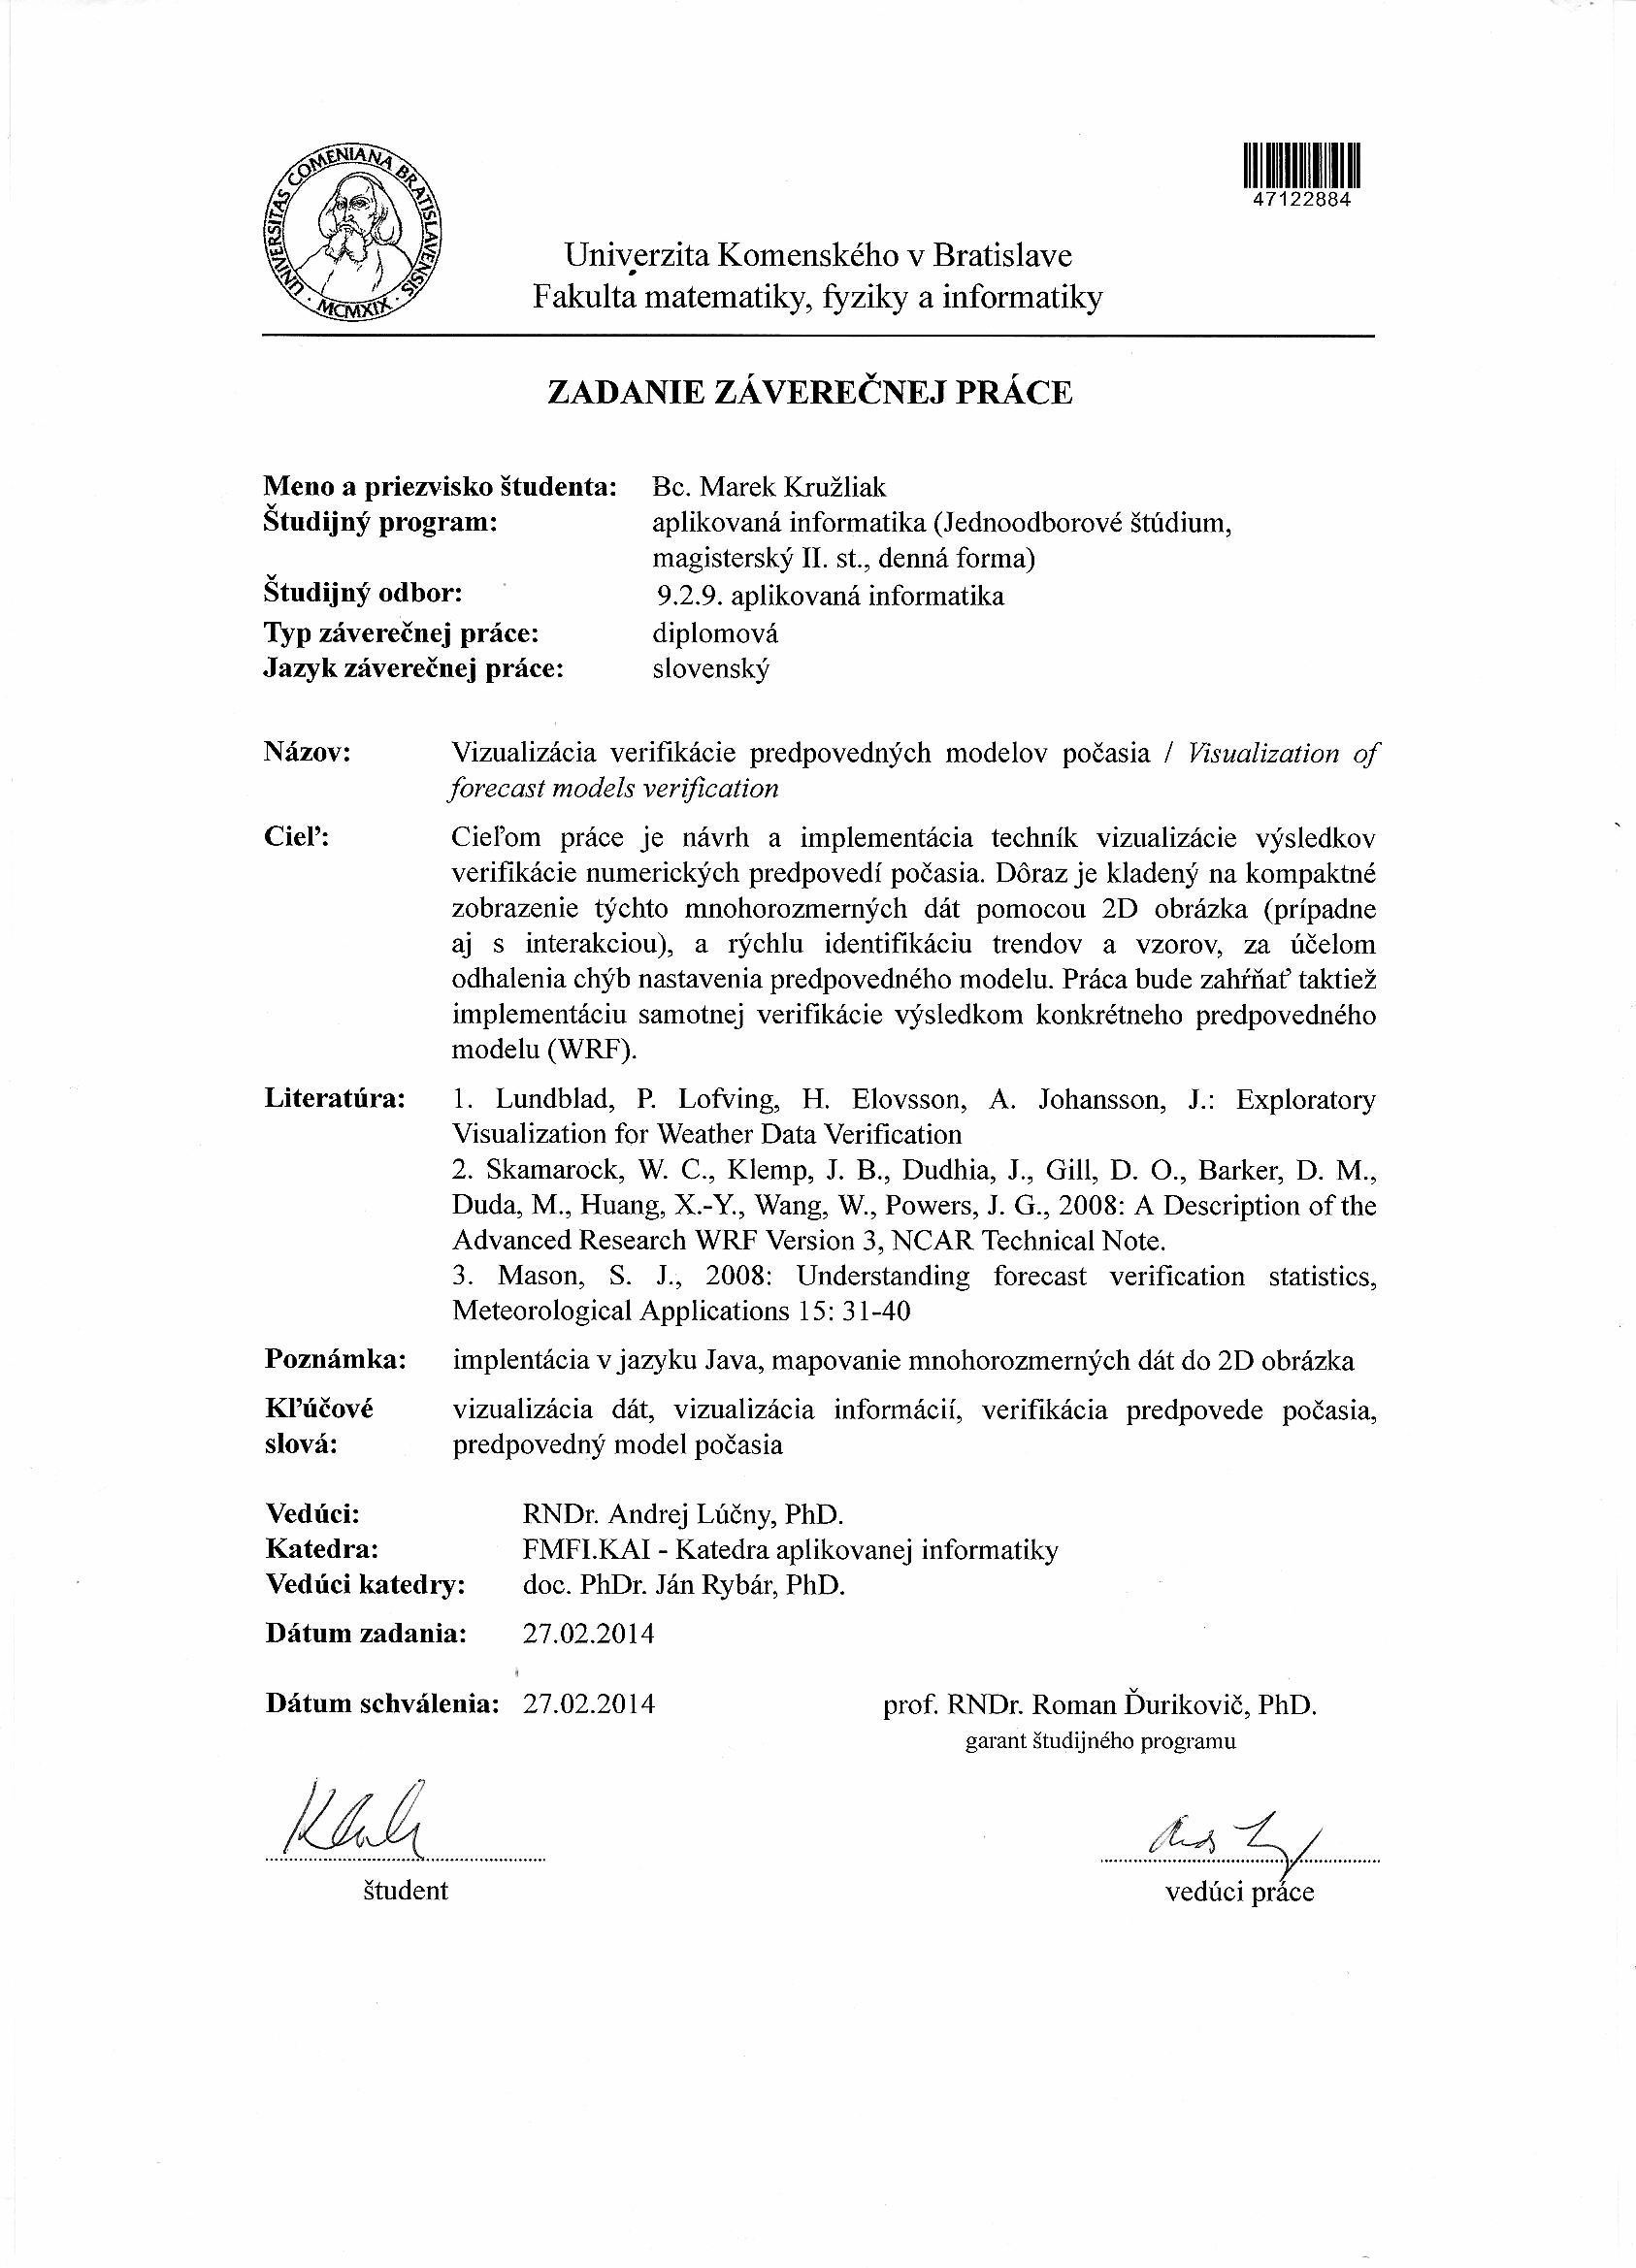
\includegraphics[width=560pt,keepaspectratio]{zadanie} %height=800pt
}
\restoregeometry
%prehlasenie
\thispagestyle{empty}
\vspace*{\fill}
\hfill
\begin{minipage}{0.63\textwidth}
Čestne prehlasujem, že som túto bakalársku prácu vypracoval samostatne s použitím citovaných zdrojov.

\bigskip
	\begin{flushright}
	\begin{minipage}{0.5\textwidth}
	\dotfill
	\end{minipage}
	\end{flushright}
\end{minipage}\eject
% Podakovanie
\thispagestyle{empty}
\topskip0pt
\vspace*{\fill}
\hfill
\begin{minipage}{0.65\textwidth}
\vspace{0pt}\raggedright
Ďakujem RNDr. Martinovi Samuelčíkovi, PhD. za to, že sa
ujal vedenia mojej bakalárskej práce a za jeho cenné rady
pri programovaní a pri písaní práce. 
\end{minipage}
\vspace*{\fill}
\eject

\setcounter{page}{1}
\pagenumbering{Roman}
% abstrakt
\begin{Huge}
\textbf{Abstrakt}  \\
\end{Huge}

Primárnym cieľom práce je opísať návrh a implementáciu praktického nástroja na tvorbu 
a editovanie voxelových objektov a scén. 
V práci sa taktiež venujeme vysvetleniu základných pojmov objemovej grafiky a jej využitiu mimo vedeckej sféry, teda v moderných herných enginoch a podobne.
Ďalej uvádzame príklady existujúcich riešení v danej oblasti, ich kladné a záporné stránky, a následné
využitie získaných poznatkov z ich testovania.
Práca taktiež opisuje zaujímavé algoritmické problémy, ktoré sa počas tvorby práce vyskytli, ich riešenie a implementáciu opísaného riešenia.\\



\textbf{Kľúčové slová:} voxel , objemová grafika, voxelizácia
\eject

\begin{Huge}
\textbf{Abstract}  \\
\end{Huge}

Primary goal of this paper is to describe design and implmentation of voxel editing tool. We also describe basic concept of volume graphics and its usage in commercial sphere, like modern game engines, animation etc. Next we mention examples of already existing solutions in this field, their strong and weak points and their influence on this work. In this paper we also analyze intersesting algorithmic problems, which appeard during implementation phase. \\

\textbf{Keywords:} voxel, volume graphics, voxelization
\tableofcontents
%zoznam obrazkov a tabuliek
\listoffigures
\begingroup
\let\clearpage\relax
\listoftables
\endgroup
%zoznam skratiek
\eject
\begin{Huge}
\noindent\textbf{Zoznam skratiek} 
\end{Huge}


\begin{figure}[!h]
		\bigskip
		\bigskip
		\hspace{0.5cm}
		\begin{minipage}[h]{0.1\textwidth}
		  WRF \\
		  NCEP \\
		  NCAR \\
		  NWP \\
		  GFS \\
		  NAM \\
		  RUC \\
		  SREF \\
		  GEFS \\
		  ECMWF \\
		  NOAA \\
		  ESRL \\
		  AFWA \\
		  NRL \\
		  CAPS \\
		  LES \\
		  WMO \\
		  TOGA \\
		  ME \\
		  MFE \\
		  MAE \\
		  RMSE \\
		  MSE \\
		  TS \\
		  MAD \\
		  GUI \\
		  VBA \\
		  SAS \\
		  CAWCR \\
		  IDL \\
		  NCL \\
		  MET \\
		  DTC \\
		  EVS \\
		  HEP \\
		  MISE \\
		  KDE \\
		  IMS \\
		  HTML \\
		  SVG \\
		\end{minipage}
		\begin{minipage}[h]{0.8\textwidth}
		  Weather Research and Forecasting \\
		  National Centers for Environmental Prediction \\
		  National Center for Atmospheric Research \\
		  Numerical Weather Prediction \\
		  Global Forecast System \\
		  North American Mesoscale Forecast System \\
		  Rapid Update Cycle \\
		  Short Range Ensemble Forecast \\
		  Global Ensemble Forecast System \\
		  European Centre for Medium-Range Weather Forecasts \\
		  National Oceanic and Atmospheric Administration \\
		  Earth System Research Laboratory \\
		  Air Force Weather Agency \\
		  Naval Research Laboratory \\
		  The Center for Analysis and Prediction of Storms \\
		  Large eddy simulation \\
		  World Meteorological Organization \\
		  Tropical Ocean Global Atmosphere \\
		  Mean Error \\
		  Mean Forecast Error \\
		  Mean Absolute Error \\
		  Root Mean Square Error \\
		  Mean Square Error \\
		  Tracking Signal \\
		  Median Absolute Deviation \\
		  Graphical User Interface \\
		  Visual Basic for Applications \\
		  Statistical Analysis Software \\
		  Centre for Australian Weather and Climate Research \\
		  Interactive Data Language \\
		  NCAR Command Language \\
		  Model Evaluation Tools \\
		  Developmental Testbed Center \\
		  Ensemble Verification System \\
		  Hydrological Ensemble Prediction \\
		  Mean Integrated Square Error \\
		  Kernel Density Estimation \\
		  Integrated Monitoring System \\
		  Hypertext Markup Language \\
		  Scalable Vector Graphics \\
		  \end{minipage}
	\end{figure}
	
\begin{figure}[!h]
		\bigskip
		\bigskip
		\hspace{0.5cm}
		\begin{minipage}[h]{0.1\textwidth}
		  CSS \\
		  CSV \\
		  UML \\
		\end{minipage}
		\begin{minipage}[h]{0.8\textwidth}
		  Cascading Style Sheets \\
		  Comma Separated Values \\
		  Unified Modeling Language \\		 
		\end{minipage}
	\end{figure}	
	 
			  
			  
			  

\eject
\setcounter{page}{1} 
\pagenumbering{arabic}

\chapter{Úvod}
	
	
Vizualizácia informácií a vizuálna analýza dát sú dnes veľmi vyvíjaným a moderným odvetvím počítačovej grafiky. Aplikácie vizualizácie informácií sú rôzne od ... cez ... až po ... Úlohou vizualizácie informácií je v prvom rade využitie ľudských kognitívnych schopností pre lepšie porozumenie dát.

Svoje využitie našla aj v procese verifikácie predpovedných modelov počasia. Dnešné metódy verifikácie predpovedí sa sústreďujú na numerický popis výkonu jednotlivých predpovedných modelov pomocou rôznorodých štatistických metód. Vo výsledku sa dáta opisujú ďalšími dátami, avšak práve na vizualizáciu týchto dát sa kladie veľmi slabý dôraz.

V našej práci sme preštudovali používané štatistické metódy pre verifikáciu spojitých premenných, ktoré predpovedá model \textit{WRF}. Hlavným cieľom práce sa však stal návrh a implementácia vizualizačných techník špeciálne navrhnutých pre potreby verifikácie. Sústredili sme sa obzvlášť na to, aby sme ušetrili cenný vizuálny priestor bez straty potrebných informácií. Návrh vizualizácie vychádza ...
\chapter{Verifikácia predpovedných modelov počasia}

Verifikácia je proces, ktorý má overiť správnosť fungovania predpovedného modelu počasia. Z tohto dôvodu je nepostrádateľnou súčasťou meteorologického výskumu a taktiež celkového procesu predpovedania počasia. \cite{MET:MET52}
Ciele verifikácie môžeme rozdeliť do troch skupín: \textit{administratívne}, \textit{vedecké} a \textit{ekonomické}.
Medzi \textit{administratívne ciele} patrí monitorovanie úspešnosti predpovedania modelu a nasmerovanie užívateľov na jeho správnu konfiguráciu alebo voľbu iného modelu. \textit{Vedeckými cieľmi} sú identifikovanie a oprava slabín modelu a taktiež vylepšovanie predpovedí. \textit{Ekonomickými cieľmi} sú rozhodovanie, kam majú smerovať investície do výskumu a iné závažné ekonomické rozhodnutia. \cite{IntroToVerif}

%TODO co sa da secko verifikovat alebo take daco...
% Standard verification methods:
% 	Methods for dichotomous (yes/no) forecasts
% 	Methods for multi-category forecasts
% 	Methods for forecasts of continuous variables
% 	Methods for probabilistic forecasts 

\section{Predpovedný model počasia}

Už v 19. storočí vývoj termodynamiky na základe Newtonovskej fyziky vyvrcholil v ucelení množiny fundamentálnych princípov, ktoré riadia prúdenie plynov v atmosfére. 
Začiatkom 20. storočia sa o matematický prístup k predpovedaniu počasia najviac zaslúžili osobnosti ako Vilhelm Bjerknes alebo Lewis F.Richardson. Avšak na ďalší úspech, v tejto oblasti, sa muselo čakať až na vynájdenie prvých počítačov počas 2. svetovej vojny ako bol IAS alebo ENIAC. \cite{Origins}
Prvá úspešná predpoveď bola vykonaná v 50. rokoch minulého storočia a to hlavne vďaka práci Jula Charneyho.
Následný vývoj vo výpočtovej sile počítačov, používanie satelitných pozorovaní a vývoj samotnej meteorológie ako vedy zapríčinil, že je numerická predpoveď počasia (NWP) dnes najúspešnejším prístupom ako predpovedať počasie.  \cite{Golding}

Odvtedy vzniklo veľké množstvo modelov, ako sú napríklad GFS, NAM, RUC, WRF, SREF, GEFS, ECMWF, ALADIN a mnoho ďalších. Naša práca sa zameriava konkrétne na verifikáciu modelu \textit{WRF}. Taktiež pokračuje neustály vývoj aj vďaka novým modelovacím technikám, novým parametrizáciám, a zvyšovaniu výkonu výpočtových zdrojov.

\begin{figure}
	\centering
	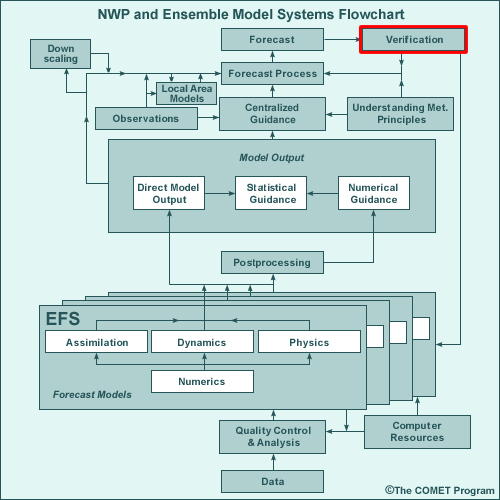
\includegraphics[width = 4in]{ForecastModelDiagramNew}
	\caption{Flowchart systému predpovedného model počasia od edukačného programu The COMET \cite{Comet}. Na obrázku je zvýraznená časť, ktorej sa venujeme v tejto práci.}
	\label{fig:fcstmodel}
\end{figure}

Ako môžeme vidieť na obrázku \ref{fig:fcstmodel} proces predpovedania počasia má okrem numerického modelu, ktorý je jej jadrom, aj iné časti. Ako príklad môžme spomenúť získavanie vstupných dát, ich predspracovanie, postprocesing, spracovanie výstupu a následne poskladanie samotnej predpovede. Cieľom nášho záujmu, celého procesu predpovedania, je \textit{verifikácia}. Ako môžme vidieť z obrázka, verifikácia vplýva na vyladenie parametrov modelu, avšak tento proces sa nedeje automaticky, ale vyžaduje prácu meteorológov a ich chápanie základných meteorologických princípov.


\subsection{WRF model}
\label{subsec:wrf}
Ako sme už spomenuli \textit{The Weather Research and Forecasting} (WRF) model je \textit{numerická predpoveď počasia} (NWP) a systém atmosferickej simulácie.

WRF je podporovaný, ako bežný nástroj pre univerzity, výskum a operačné komunity, pričom sa usiluje o splnenie požiadaviek ich všetkých súčasne.
Vývoj WRF modelu bol snahou mnohých spoločností ako napríklad \textit{The National Center for Atmospheric Research’s} (NCAR), \textit{Mesoscale and Microscale
Meteorology} (MMM), \textit{The National Oceanic and Atmospheric Administration’s} (NOAA) \textit{National Centers for Environmental Prediction} (NCEP) a \textit{Earth System Research Laboratory} (ESRL), oddelenie ministerstva obrany \textit{Air Force Weather Agency} (AFWA) a \textit{Naval
Research Laboratory} (NRL), \textit{The Center for Analysis and Prediction of Storms} (CAPS) \cite{WRF}. 

WRF model je vhodný pre širokú škálu aplikácií od \textit{metódy vzdušných vírov} (Large Eddy Simulation - LES) až po globálne simulácie počasia. Takéto aplikácie vyžadujú numerické predpovede v reálnom čase, vývoj a štúdium asimilácie dát, výskum parametrizovanej fyziky, výskum parametrizovanej fyziky ,modelovanie kvality ovzdušia, idealizované simulácie, čo všetko WRF model spĺňa.

V roku 2008 evidovala WRF viac ako 6000 užívateľov, no dnes (2014) eviduje viac ako 25000 užívateľov vo viac ako 130 krajinách sveta. Tieto fakty poukazujú na to, že WRF model má nie len veľkú základňu užívateľov, ale aj vývojárov a má v budúcnosti istotne svoje miesto a preto si myslíme, že sa oplatí investovať čas a úsilie do verifikácie tohto modelu.

\section{Dáta}
\label{sec:data}
Na správne zhodnotenie úspešnosti modelu potrebujeme dva druhy dát. V prvom rade sa jedná o dáta, ktoré sú výstupom z daného predpovedného modelu počasia, teda \textbf{predpovedané dáta}. Tieto umelo získané dáta chceme konfrontovať s realitou, aby sme si mohli vytvoriť obraz o správnom fungovaní celého modelu. Realitu v našom prípade predstavujú dáta namerané špecializovanými meteorologickými senzormi, ktoré označujeme ako \textbf{pozorované dáta} alebo skrátene \textit{pozorovania}.  

\subsection{Predpovedané dáta}
Predpovedané dáta z modelu WRF sa ukladajú vo formáte \textbf{GRIB}, čo je skratka pre \textit{GRIdded Binary} \cite{GRIB} alebo na iných miestach uvádzané ako \textit{General Regularly-distributed Information in Binary form} \cite{GRIB12}. Tento formát je štandardom Svetovej meteorologickej organizácie teda \textit{World Meteorological Organization} (WMO). Jedná sa o pomerne rozšírený formát, používaný pri veľkom množstve meteorologických aplikácií a je taktiež používaný ako výstupný formát pre iné predpovedné modely ako WRF, či už ECMWF, GFS, NAM, SREF alebo mnohé iné \cite{Products}.

Doteraz boli vyvinuté 3 verzie tohoto formátu od 0 po 2. Verzia 0 bola určená pre malé projekty typu TOGA a to iba s limitovaným použitím a dnes sa táto verzia už vôbec nepoužíva. Verzia grib 1 \cite{GRIB}, grib 2 \cite{GRIB12} sú dnes bežne používané väčšinou meteorologických centier.

Medzi verziami 1 a 2 nie sú žiadne rozdiely v obsahovej filozofii, preto popis obsahu gribovského formátu, ktorý tu uvádzame je spoločný pre obe tieto verzie. 
\textit{Gribovský súbor} (ďalej iba \textit{Grib}) pozostáva z viacerých \textit{Gribovských záznamov}, pričom jeden záznam môže existovať ako samostatný Grib. Vďaka tomu je možné ľahko spájať Griby, a to tiež v ľubovoľnom poradí, bez toho, aby sme ich nejako poškodili. Samozrejme musí byť zachovaná homogenita, čo sa týka verzií Gribov, teda verziu 1 nemožno miešať s verziou 2 a naopak.
Už samotný názov \textit{Gridded Binary} nám napovedá, že dáta sú usporiadané v pravidelnej mriežke. Každý Gribovský záznam obsahuje dvojrozmernú mriežku (zemepisná šírka x zemepisná dĺžka) hodnôt v určitom čase a vertikálnej hladine. Taktiež v hlavičke záznamu sa nachádzajú metainformácie, ktoré nám hovoria o aké dáta ide, teda o akú premennú sa jedná, čas predpovede, výškovú hladinu a podobne. Grib je zvyčajne z tohto dôvodu 2 až 5 rozmerná dátová štruktúra s veľkým množstvom veličín ako je napríklad teplota, tlak, relatívna vlhkosť, rosný bod, \textit{u} a \textit{v} súradnice vetra a ďalšie, ktoré sú definované v rôznych hladinách. Taktiež je dôležité povedať, že Grib zriedkakedy zachytáva povrch celej planéty, ale iba vymedzenú skúmanú oblasť - \textit{doménu}.

\subsection{Pozorované dáta}
Pozorovania sa získavajú meraním priamo v teréne pomocou špecializovaných meracích zariadení, ktoré sú súčasťou meteo staníc. Každá stanica môže obsahovať iné vybavenie, ku príkladu teplomer, zrážkomer, barometer, vetromer a im podobné \cite{WeatherStation}, ktorými môžme zachytávať informácie o rôznych skúmaných veličinách. 
%http://www.weathergraphics.com/dl/obsman.pdf
% http://en.wikipedia.org/wiki/Weather_station

Majoritná časť meraní sa deje pri povrchu zeme priamo na meteo staniciach a nazývajú sa \textit{surface} merania. Tieto merania najlepšie popisujú dianie v oblasti najväčšieho záujmu (biosfére), avšak neobsahujú informáciu o dianí v iných výškových hladinách. Pozorovania týchto hladín sa dejú pomocou \textit{radiosondy}, ktorá je pripojená k meteo balónu alebo vypustená z lietadla smerom k zemi. Takéto pozorovania sa nazývajú \textit{upper air} merania.

Narozdiel od predpovedaných dát, pozorované dáta nemajú štandardizovaný formát a zvyčajne sa ukladajú do databázy.
Aby sme zhrnuli charakteristiku týchto dát, jedná sa o niekoľko meraných veličín, nameraných v konštantných časových krokoch - napríklad každú minútu alebo každú hodinu - v jednom konkrétnom geografickom bode a zvyčajne pri povrchu zeme, teda ak sa nejedná o upper air merania, ktoré sa uskutočňujú v štandardných výškových hladinách, ktoré sa merajú v hPa.

\subsection{Párovanie dát}
\label{subsec:pairing}
%TODO novy pristup
Z predpovedného modelu a rovnako aj z merania získame veľké množstvo hodnôt. Aby sme mohli korektne porovnať predpovede s pozorovaniami, je nevyhnutné nájsť správne párovanie týchto hodnôt, teda zistiť, ktorú hodnotu porovnať s ktorou, aby sme získali zmysluplný výsledok.

Vždy sa snažíme nájsť správnu predpoveď pre pozrovanie a nie naopak.
% Vzhľadom na charakter dát sa 
Dôvodom je, že chceme skúmať vzťah predpovede s realitou a preto v párovaní musí byť zahrnutých čo najviac \textbf{meraných} hodnôt, ak nie všetky.

Každá pozorovaná hodnota, ktorú chceme spárovať má štyri kľúče podľa ktorých hľadáme pár: \textit{meraná veličina} (napríklad teplota), \textit{čas merania}, \textit{výšková hladina} a \textit{geografická poloha}.
Nájsť všetky hodnoty podľa kľúča meranej veličiny v Gribe je ľahké, keďže sa jedná o kategorickú premennú, teda môže nadobúdať iba určitý konečný počet hodnôt. Toto sa však nedá povedať o čase, hladine a polohe, ktoré sú spojitými premennými.
 
Pre čas pozorovania, čas predpovede a výškovú hladinu existujú štandardy, ktoré určujú v akých časoch resp hladinách sa robia merania a predpovede, čo nám uľahčuje prácu. Ak sa napriek tomu čas alebo hladina v Gribe nevyskytuje, tak pár vyhadzujeme z párovania. 

V prípade polohy zo samozrejmých dôvodov neexistuje žiaden štandard a hustota mriežky v Gribe nemôže byť nikdy tak veľká, aby poloha našej stanice vždy dopadla na presný bod mriežky. Z tohoto dôvodu získavame hodnoty z mriežky z okolitých bodov a to dvoma metódami \textit{Point-to-Grid} a \textit{Grid-to-Point} \cite{IntroToVerif}, ktoré sú znázornené na obrázku \ref{fig:pointmethods}. Jedná sa vlastne o dve interpolačné metódy. Point-to-Grid predstavuje metódu \textit{najbližší sused} (\textit{Nearest Neighbour}) a Grid-to-Point \textit{bilineárnu interpolačnú metódu}. 

Výber správnej metódy môže značne ovplyvniť výsledok. Dôvodom je, že môžu byť veľké rozdiely hodnôt v okolitých mrežových bodoch a tak, ak pomocou Point-To-Grid metódy získame nízku hodnotu, tak pomocou Grid-To-Point môžeme získať hodnotu omnoho väčšiu, vplyvom zvyšných troch bodov, ktoré vstúpili do interpolácie. Nemožno však jednoznačne povedať, ktorá z metód je lepšia, keďže obe môžu v istých prípadoch dávať lepšie výsledky. 

\begin{figure}
	\centering
	\begin{tabular}{ c c }
	\subfloat[Point-to-Grid]{\includegraphics[width = 2.5in]{PointtoGrid}} &
	\subfloat[Grid-to-Point]{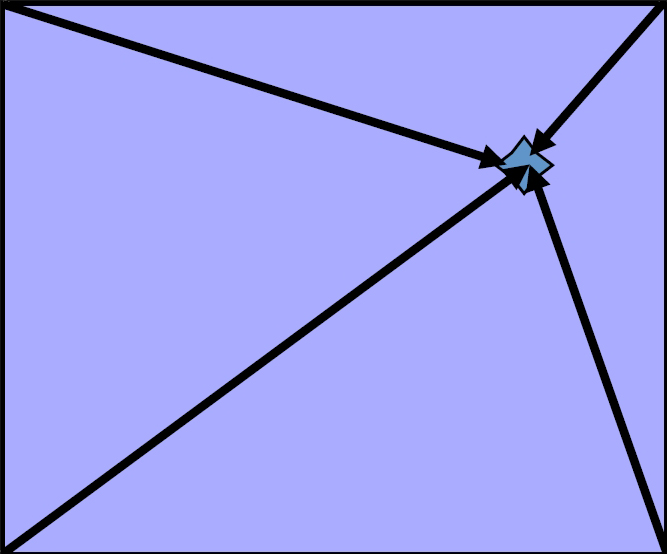
\includegraphics[width = 2.5in]{GridToPoint}} 
	\end{tabular}

	\caption{Vizuálne znázornenie dvoch bežne používaných metód na získavanie hodnôt z mriežky}
	\label{fig:pointmethods}
\end{figure}

\section{Meranie chyby predpovede}
\label{sec:errormeasurement}
Výsledkom procesu párovania je $n$ párov (predpoveď, pozorovanie), ktoré je možné porovnať. Z porovnania týchto dvojíc získame numerickú hodnotu, ktorá nám hovorí o veľkosti chyby predpovede daného modelu pre vybrané predpovedané časy.
\\
Chybu predpovede $e_i$ pre $i$-tu dvojicu $(y_i, \hat{y}_i)$ definujeme takto: 
\[  
	e_i = (y_i - \hat{y}_i)
\]
Kde $ y_i $ je predpoveď a $ \hat{y}_i $ je pozorovanie.
Takýmto spôsobom z $ n $ párov získame $ n $ chýb, ktoré agregujeme pomocou rôznych štatistických metód, ktoré sú bežne používané pri verifikácií predpovedí, ako sa spomína v \cite{RecommendOnVerif}, \cite{IntroToVerif} a \cite{ContinuousVerif}. Výsledkom agregácie je numerická hodnota, ktorá sa nazýva \textit{skóre} predpovede. 

\subsection{Stredná chyba predpovede}
Budeme ju označovať ako \textit{MFE} z anglického \textit{Mean Forecast Error}, ale v literatúre je možné ju nájsť ako \textit{ME} \cite{RecommendOnVerif}, teda \textit{stredná chyba} alebo ako \textit{Linear Bias} \cite{ContinuousVerif}, \cite{IntroToVerif}. Vzorec pre výpočet MFE vyzerá nasledovne:
\[
	MFE = \frac{1}{n}\sum\limits_{i=0}^{n}  e_i  
\]
MFE je možné vypočítať aj ako rozdiel priemerov predpovedí a pozorovaní.
\[
	MFE = \bar{y} - \bar{\hat{y}}  
\]
MFE vyjadruje priemerný smer chyby. To znamená, že pozitívny výsledok indikuje \textit{over-forecast}, teda nadhodnotenú predpoveď a negatívny výsledok \textit{under-forecast}, teda podhodnotenú predpoveď. Avšak MFE \textbf{nevyjadruje veľkosť} chyby v tomto smere, keďže kladné a záporné chyby sa navzájom môžu zrušiť. 
Napríklad máme množinu chýb $ E = \{2, -5\} $, tak MFE pre $ E $ je -1.5, ale priemerná veľkosť chyby je 3.5.  

\subsection{Stredná absolútna chyba}
Budeme ju označovať ako \textit{MAE} z anglického \textit{Mean Absolute Error}. Vzorec pre výpočet MAE vyzerá nasledovne:
\[
	MAE = \frac{1}{n}\sum\limits_{i=0}^{n} \lvert e_i \rvert 
\]
Narozdiel od MFE \textbf{neurčuje smer chyby}, ale vyjadruje veľkosť chyby. Z týchto dôvodov je v praxi odporúčané zobrazovať MFE a MAE súčasne \cite{RecommendOnVerif}. 

\subsection{Stredná kvadratická chyba}
Budeme ju označovať ako \textit{RMSE} z anglického \textit{Root Mean Square Error}. Vzorec pre výpočet RMSE vyzerá nasledovne:
\[
	RMSE = \sqrt{ \frac{1}{n}\sum\limits_{i=0}^{n} e_i^{2}  }
\]
Z povahy vzorca pre RMSE je jasné, že rovnako ako MAE, ani RMSE neurčuje smer chyby, pretože nadobúda vždy iba kladné hodnoty. 
Ďalšou vlastnosťou RMSE je, že nadobúda hodnoty vždy väčšie alebo rovné ako MAE, pričom výsledok RMSE je citlivý na veľké hodnoty chýb. \\
\label{subsec:mse}
V praxy sa zvykne používať aj \textit{MSE} (\textit{Mean Square Error}):
\[
	MSE = \frac{1}{n}\sum\limits_{i=0}^{n} e_i^{2} 
\]
Má podobné vlastnosti ako RMSE s jediným rozdielom, že RMSE meria veľkosť chyby zachovávajúc jednotky danej veličiny (napr. \textcelsius), zatiaľ čo MSE jednotky nezachováva \cite{RecommendOnVerif}. Preto sme si pre náš účel zvolili RMSE, ktoré je jednoduchšie zobraziť spolu s MFE a MAE v jednom grafe, keďže sa zachováva konzistentnosť jednotiek veličín.



%\subsection{Signál chybných predikcií}
%\[ 
%	TS = \frac{\sum\limits_{i=0}^{n} e_i}{MAE}
%\]

\subsection{Všeobecná kumulovaná chyba}
\label{subsec:cumulativeerror}
V našom systéme sme navrhli všeobecný vzorec na výpočet kumulovaného skóre, ktorým možno vyjadriť ľubovoľnú zo spomenutých štatistických metód. Takéto vyjadrenie umožňuje nie len všeobecnosť, ale aj jednoduché rozšírenie systému o ďalšie metódy a to nie len programátorom, ale aj samotným užívateľom systému.
\\
Všeobecný vzorec na výpočet \textit{skóre} pre danú predpoveď vyzerá takto:
\[
	Score = \Phi(\sum\limits_{i=0}^{n} \varepsilon(e_i))  
\]
Kde $ \Phi $ je ľubovoľná funkcia z $\mathbb{R}$ do $\mathbb{R}$, teda $ \Phi : \mathbb{R} \rightarrow \mathbb{R} $ a podobne funkcia $ \varepsilon : \mathbb{R} \rightarrow \mathbb{R} $.
Spomenuté metódy môžme teda skonštruovať zadefinovaním správneho $ \Phi $ a $ \varepsilon $. \\
Napríklad pre \textit{MFE}:
\[ \Phi(x) = \frac{x}{n} \]
\[ \varepsilon(e) = e \] 
Pre \textit{MAE}:
\[ \Phi(x) = \frac{x}{n} \]
\[ \varepsilon(e) = \lvert e \rvert \]
Pre \textit{RMSE}:
\[ \Phi(x) = \sqrt{\frac{x}{n}} \]
\[\varepsilon(e) = e^2 \]
Pre \textit{MSE}:
\[ \Phi(x) = \frac{x}{n} \]
\[ \varepsilon(e) = e^2 \] 

Ako sme spomenuli, je možné rozšírenie o ďalšie metódy a to napríklad o Brownov a Triggov \textit{signál chybných predikcií}, ktorý budeme označovať ako \textit{TS} z anglického \textit{Tracking Signal}. Tieto metódy sme vyššie nespomenuli, keďže sa v meteorologickej praxi nepoužívajú. Uvádzame ich však ako možné rozšírenie, keďže sú tieto metódy bežne používané pri verifikácii iných predpovedných modeloch, ako sú tie meteorologické.

\subsection{Medián absolútnych chýb}
\label{subsec:mad}
Budeme ju označovať ako \textit{MAD} z anglického \textit{Median Absolute Deviation}. Vzorec pre výpočet MAD vyzerá nasledovne:
\[
	MAD = median( \lvert e  \rvert) = \tilde{ \lvert e  \rvert}
\]
Nech je daná usporiadaná postupnosť $ Y_1, \ldots , Y_N $, tak potom $ median $ náhodnej premennej $ x $ je definovaný rovnako ako v \cite{StatMedian}:
\[
	median(x) = \tilde{x} \equiv \left\{
		\begin{array}{ll}
			Y_{(N+1)/2}  & \mbox{ak } N\mod{2} = 0 \\
			\frac{1}{2}(Y_{(N+1)/2} + Y_{(N+1)/2 + 1}) & \mbox{ak } N\mod{2} = 1
		\end{array}
	\right.
\]
Z daného vzorca môžeme vidieť podobné vlastnosti ako má MAE, avšak MAD je robustnejší a extrémne chyby nemajú na skóre žiaden efekt.

%TODO pridat LEPS - http://www.cawcr.gov.au/projects/verification/LEPS.php
% preto treba aj zmenit nejake veci 
\Chapter{Predchádzajúce riešenia 1}{Verifikačný softvér}

Verifikácia predpovedných modelov počasia je úloha dokonale stvorená pre automatizáciu. 
Z tohto dôvodu meteorológovia začali využívať dostupný štatistický softvér 
a neskôr boli taktiež vyvíjané špecializované nástroje určené pre verifikáciu.
Môžeme teda rozdeliť verifikačný softvér do dvoch základných kategórií a to \textit{štatistický} a \textit{špecializovaný}, ktorý je zväčša podporovaný rôznymi národnými a medzinárodnými organizáciami.

\section{Štatistický softvér}
%TODO
Spoločnou črtou: \\
	- obmedzená funkcionalita \\
	- obmedzená vizualizácia \\
	- slabé / žiadne GUI \\
	- vyžaduje znalosť špecifického programovacieho jazyka \\
	- ...


\subsection{Tabuľkový softvér}
Napriek tomu, že je tabuľkový softvér na výpočet štatistík zamietnutý komunitou vedcov a štatistikov ako nevhodný a neprofesionálny, tak je využívaný, a to pomerne často, aj vo vedeckých kruhoch. 
Výhodou je, že novému užívateľovi umožňuje okamžite vidieť všetky kroky v základných procedúrach verifikácie a teda je výborný pre výučbové účely. \cite{VerifSoft} 
Najznámejší kus softvéru z pomedzi komerčných produktov je \textit{Microsoft Excel} \cite{Excel} a z voľne dostupných je jeho opensoruce náprotivok \textit{Open Office Calculate} \cite{OpenOfficeCalc}. Oba programy zahrňujú základné štatistické funkcie ako napríklad stredná kvadratická chyba (\textit{MSE}) pre spojité predpovede (pozri odsek \ref{subsec:mse}) a taktiež umožňujú generovanie jednoduchých grafov na základe tabuľkových dát. Tabuľkový softvér neposkytuje priamo funkcionalitu na výpočet ďalších sofistikovanejších verifikačných štatistík, avšak umožňuje ich implementáciu pomocou makro programovania v špecifickom jazyku. Pre Microsoft Excel je to \textit{Microsoft Visual Basic for Applications}(VBA) \cite{VBA} a pre Open Office Calculate zasa \textit{OpenOffice.org Basic} \cite{OpenOfficeBasic}. Oba jazyky patria do rodiny \textit{Basic} jazykov, takže majú mnoho podobných prvkov.  


\subsection{MATLAB}
\textit{MATLAB} je interaktívne prostredie s vlastným programovacím jazykom, ktorý je využívaný miliónmi inžinierov a vedcov po celom svete \cite{Matlab} a tým nevynímajúc meteorológov a ďalších odborníkov pracujúcich v atmosférickom výskume. 
Zvyčajne sa MATLAB využíva na výskum a protoypovanie nových metód a procedúr \cite{VerifSoft}, pretože umožňuje rýchlu a jednoduchú implementáciu, keďže jeho súčasťou je mnoho matematických knižníc a je prispôsobený na prácu s maticami dát.
Výhodou MATLABU je, že umožňuje tvorbu GUI a taktiež poskytuje kreslenie rôznorodých grafov a diagramov.
Mali by sme však podotknúť, že podobne ako väčšina štatistického softvéru, aj \textit{MATLAB} je komerčný produkt. Jeho cena za jednu licenciu je \$2,650 (k roku 2015), čo je pomerne vysoká suma, ak vezmeme do úvahy za akým účelom chceme tento softvér využívať a ako dobre je naň prispôsobený.

\subsection{R}
Často používaným a pomerne mocným nástrojom je \textit{open source} skriptovací jazyk \textit{R} [www.r-project.org]. V posledných desaťročiach sa stal dominantným jazykom v oblasti štatistického výskumu. Napriek tomu, že ide o voľne stiahnuteľný softvér, tak jeho základný balík obsahuje všetky funkcie, ktoré obsahujú aj platené produkty. R-ko však nezostáva len pri tom, pretože v dobe písania tejto práce (marec 2015) bolo dostupných vyše 6400 užívateľských balíkov s rôznorodou funkcionalitou. Pre nás je dôležití, že medzi týmito balíkmi sa objavil aj balík určený na verifikáciu s názvom \textit{\textbf{verification}} [NCAR, 2010]. Tento balík obsahuje základné funkcie verifikácie na výpočet štatistík pre spojité, kategorické ale i pravdepodobnostné predpovede. 

Jazyk R neslúži iba na rôznorodé štatistické výpočty, ale poskytuje aj veľmi dobre parametrizovateľnú vizualizáciu. V balíkoch jazyka sa nachádzajú funkcie pre čiarové diagramy, krabicové diagramy, bodové grafy a mnohé iné komplexnejšie vizualizácie, ale taktiež funkcie na zobrazenie základných vizuálnych prvkov, ktorými možno vytvoriť úplne novú osobitnú vizualizáciu.

\subsection[SAS]{Statistical Analysis Software (SAS)}
\textit{Statistical Analysis Software} \cite{SAS}, skrátene SAS, je opäť štatistický programovací jazyk aj so svojim vývojovým prostredím. V oblasti bioštatistiky a farmakológie je veľmi uznávaným a často používaným jazykom. Keďže je veľká podobnosť v používaných metódach medzi verifikáciou predpovedí a spomínanými odvetviami \cite{VerifSoft}, SAS poskytuje funkcionalitu použiteľnú aj pre verifikáciu. Okrem iného SAS ponúka základné, ale aj niektoré pokročilejšie nástroje na vizualizáciu dát. Opäť však musíme podotknúť, že ide o komerčný produkt, ktorého cena licencie je pomerne vysoká.

\subsection[IDL]{Interactive Data Language (IDL)}
IDL, teda \textit{Interactive Data Language} je opäť jeden z matematických programovacích jazykov, ktoré patria medzi menej používané v komunite atmosferického výskumu. Napriek tomu niektorí výskumníci medzi, ktorými je aj \textit{Beth Ebert} z \textit{Centre for Australian Weather and Climate Research} (CAWCR) uverejnili na svojich webstránkach kód obsahujúci metódy verifikácie napísané v IDL:
\begin{itemize}
	\item Metódy pre verifikáciu pravdepodobnosti zrážok 	(\url{http://www.cawcr.gov.au/projects/verification/POP3/POP3.html})
	\item Priestorové metódy (\url{http://
		www.cawcr.gov.au/staff/eee/#Interests})
\end{itemize} 
IDL na používanie požaduje taktiež získanie platenej licencie, čo obmedzuje počet užívateľov a rovnako aj zdieľanie kódu medzi, ktorý by si mohol ktokoľvek spustiť.


\section{Špecializovaný softvér}

\subsection[NCL]{NCAR Command Language (NCL)}
Ako väčšina softvérových riešení v predchádzajúcej sekcii, tak aj \textit{NCL}, teda \textit{NCAR Command Language} \cite{NCL http://www.ncl.ucar.edu/} je skriptovací jazyk s vlastnou syntaxou a interpreterom. Ide o voľne šíriteľný produkt od \textit{National Center for Atmospheric Research} (NCAR), a jeho zameranie je pochopiteľne na atmosferický výskum. Jeho primárnym cieľom je spravovanie a manipulácia klimatologických dát z predpovedných modelov, čo je jedna zo základných častí verifikácie. NCL obsahuje balík funkcií, ktorými je ľahké implementovať štatistiky verifikácie spojitých premenných, ktoré sme spomínali v časti \ref{sec:errormeasurement}. 

Súčasťou jazyka je aj možnosť vizualizácie predpovedných dát, ale taktiež aj niektoré jednoduché štatistické vizualizačné nástroje použiteľné vo verifikácii. Vzhľadom na to, že ide o meteorologický softvér, tak množstvo funkcií slúžiacich na verifikáciu je nedostačujúci, čoho príčinou môže byť, že verifikácia predpovedných modelov je ešte stále vo svojich začiatkoch \cite{VerifSoft}. Sme si istý, že ako metódy aj používané praktiky pokročia, tak budú vytvorené komunitou NCL vytvorené na tento účel funkcie.

\subsection[MET]{Model Evaluation Tools (MET)}
MET was developed by and is supported at the National Center for Atmospheric Research (NCAR) by the Developmental Testbed Center (DTC) with funding from the US Air Force Weather Agency and NOAA. The tool has been designed to work directly with versions of the Weather Research and Forecasting (WRF) modelling system, but can be modified to be useful for other types of forecasts. Much of the analysis presented in Chapter 6 utilized MET. MET provides a variety of verification techniques, including:\\
 
 Standard verification scores comparing gridded model data to point-based observations. \\
 Standard verification scores comparing gridded model data to gridded observations. \\
 Spatial verification methods comparing gridded model data to gridded observations using neighbourhood, object-based and intensity-scale decomposition approaches. \\
 Probabilistic verification methods comparing gridded model data to point-based or gridded observations. \\
 
Another powerful addition to MET is the MODE tool. MODE provides object-based methods to identify and match forecasts and observations – matching them by treating them as geometrical features. Figure 6.8 was created using MODE. Strengths of MET include the strong institutional support provided to method development, instruction and research. This includes biannual MET tutorials, which accompany WRF tutorials taught at NCAR. Additionally, there is an annual MET workshop that focuses on newdevelopments inMET. The project is open source and available to researchers from most countries (subject to US trade restrictions). MET uses a number of libraries created by other organizations to read and process data. This requires that a number of libraries be installed locally on the user’s machine. While many systems are supported, installation is an issue. In general, while MET may be an extremely useful tool for people familiar with operating and conducting research in numerical weather forecasts, the system has a steep learning curve for

\subsection[EVS]{Ensemble Verification System (EVS)}


\section{Zhrnutie}
V tejto časti sme sa snažili prehľadným spôsobom v tabuľke \ref{tab:XY} zhrnúť porovnanie spomenutého softvéru využívaného pri verifikácii.
%TODO tabuľka softvéru

\Chapter{Predchádzajúce riešenia 2}{Techniky vizualizácie vo verifikácii}
\label{chap:prevvis}

\section{Bodový graf}
\label{sec:scatterplot}
Najjednoduchším spôsobom ako analyzovať vzťah dvoch náhodných premenných je \textit{bodový graf}, ktorý je inak nazývaný aj \textit{korelačný diagram} a známy je tiež pod svojim anglickým pomenovaním \textit{scatter plot}. Bodový graf je vhodný na štúdium kolerácie dvoch premenných a taktiež je výborný pri odhaľovaní takzvaných \mbox{\textit{outlier}-ov}, teda hodnôt, ktoré sa nejakým spôsobom výrazne odlišujú od tých ostatných. Taktiež nám nepriamo podáva správu o distribúcii hodnôt, čo však pri ich veľkom počte môže byť skreslené, keďže sa body začnú postupne prekrývať, a tak nemožno určiť v akej oblasti je viacej, či menej bodov. Tento jav sa nazýva \textit{overplotting}.


\subsection{Konštrukcia bodového grafu}
Skonštruovanie bodového grafu je veľmi jednoduché a aj preto je často používaným prostriedkom na vizualizáciu. Na svoju konštrukciu využíva karteziánsku sústavu súradníc. Dve náhodné premenné, ktoré chceme porovnať, vizualizujeme tak, že spravíme zobrazenie jednej premennej na \mbox{$ x $-ovú} súradnicovú os a zobrazenie druhej premennej na \mbox{$ y $-ovú} os. Následne v danom bode nakreslíme určený symbol, čo zvyčajne býva čierna bodka alebo krúžok. 
Na obrázku \ref{fig:scattervsqq}a) vidíme príklad výsledného bodového grafu, ktorý vznikne takýmto postupom.

Bodový graf ponúka mnoho spôsobov, ako pridať ďalší rozmer informácie do vizualizácie. Môžeme zvoliť odlišnú súradnicovú sústavu, čím veľmi jednoducho vytvoríme napríklad 3D bodový graf pre trojrozmerné dáta. Ďalšou možnosťou rozšírenia je zmena vykresľovaného symbolu, ktorému môžme nastavovať rôzne parametre, do ktorých možno zakódovať nové informácie. Zvyčajne sú týmito parametrami farba, \mbox{alfa-transparencia} \cite{SolutionToOverplotting}, veľkosť \cite{Viegas}, tvar \cite{GenSensScatterplot, EnhanceScatterplot} a podobne. Tieto modifikácie si v komunite vizuálnej analýzy vyslúžili aj vlastné názvy a teoretické zázemie, avšak v našej práci sa týmto druhom diagramov nebudeme venovať.

\subsection{Kantil-kvantil graf}
\label{subsec:qqplot}
Dôležitou a často využívanou variáciou pre bodový graf je \textit{kvantil-kvantil graf}, skrátene \textit{\mbox{Q-Q} graf} (Q z anglického \textit{quantil}). Jediným rozdielom medzi bodovým grafom a \mbox{Q-Q} grafom je, že zatiaľ, čo bodový graf vizualizuje surové dáta, \mbox{Q-Q} graf zobrazuje iba kvantily z oboch dátových množín. 

Kvantilmi sú hodnoty, ktoré rozdeľujú usporiadanú dátovú množinu na niekoľko rovnako veľkých častí. Pre jednu dátovú množinu je $ (q - 1) $ $ q $-kvantilov. Najznámejším príkladom je \mbox{2-kvantil}, ktorý sa nazýva medián. Ďalšími bežnejšie používanými sú \mbox{4-kvantily}, \mbox{10-kvantily} a \mbox{100-kvantily}, čo sú vlastne kvartily, decily a percentily. 

To, čo sa zvyčajne robí pri \mbox{Q-Q} grafe je, že sa nevyberá konkrétny typ kvantilu, ale hodnoty sa jednoducho usporiadajú podľa veľkosti a zobrazia. Ak máme množinu $ A $ a jej veľkosť je $ n = \lvert A \rvert $, tak vizualizjeme $ n $ \mbox{$ q $-kvantilov}, kde $ q = n + 1 $.  Tým, že nezobrazujeme na grafe surové dáta, ale kvantily, \mbox{$ k $-ty} bod v grafe nie je zobrazením \mbox{$ k $-teho} páru hodnôt, ako to bolo v klasickom bodovom grafe, ale zobrazením \mbox{$ k $-teho} \mbox{$ q $-kvantilu}. 

Na obrázku \ref{fig:scattervsqq} môžme vidieť porovnanie bodového grafu a \mbox{Q-Q} grafu pre rovnakú dátovú množinu.


\begin{figure}
	\centering
	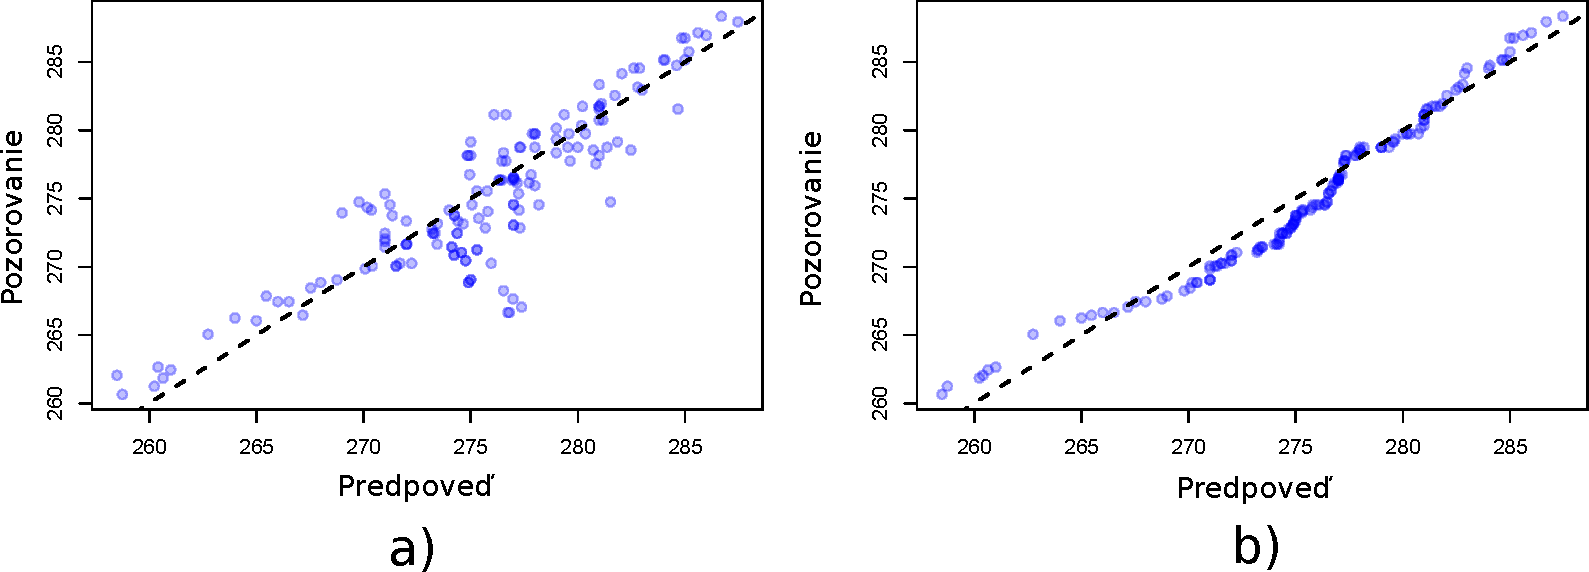
\includegraphics[width = 5.5in]{scattervsqq}
	\caption{Porovnanie bodového grafu a Q-Q grafu pre rovnaké dáta. Oba grafy boli vygenerované v programe EVS \cite{EVS}. a) Bodový graf b) Q-Q graf }
	\label{fig:scattervsqq}
\end{figure}

\subsection{Úloha bodového grafu vo verifikácii}
Úloha bodového grafu a \mbox{Q-Q} grafu vo verifikácii je rovnaká, avšak oba nám dávajú trocha iný pohľad na dáta. Vo všeobecnosti nám tieto dva grafy dávajú informáciu o vzťahu medzi dvoma veličinami, ich korelácii a taktiež aj o ich distribúcii. 

Dôležitým faktorom teda zostáva aké premenné umiestnime na \mbox{$ x $-ovú} a aké na \mbox{$ y $-ovú} os. Vo verifikácii predpovedných modelov počasia sú to zvyčajne predpovede na jednej osi a pozorovania na druhej. Taktiež sa zvyknú robiť dvojice (predpoveď, chyba predpovede), (pozorovanie, chyba predpovede) alebo (čas predpovede, chyba predpovede) a im podobné. V našej aplikácii sme testovali poslednú zo spomenutých dvojíc.

\section{Krabicový diagram}
\label{sec:boxplot}
Krabicový diagram je v anglickej literatúre zvyčajne nazývaný \textit{box plot} alebo na niektorých miestach označovaný tiež ako \textit{box and whisker\footnote{Slovo \textit{whisker} znamená po slovensky fúz, čo naznačuje, že čiary, ktoré spájajú horný a dolný kvartil s hraničnými hodnotami pripomínajú fúzy.} plot}. Odkedy bol prvýkrát publikovaný v roku 1977 \cite{Tukey}, uplynulo už takmer 40 rokov a dnes ho považujeme už za štandardnú techniku ako vizualizovať distribúciu hodnôt kompaktným spôsobom. Na svoju reprezentáciu využíva súbor 5 čísel (tzv. \textit{\mbox{5-number} summary}) \cite{Potter}, ktoré charakterizujú distribúciu dát robustným spôsobom. Tým, že zredukujeme zvyčajne veľkú dátovú množinu na týchto pár hodnôt ušetríme nielen vzácny vizuálny priestor \cite{Wickham}, ale taktiež námahu analytika, ktorý sa snaží preskúmať iba niektoré vybrané charakteristiky. 

\subsection{Konštrukcia krabicového diagramu}

Na zostavenie krabicového diagramu potrebujeme týchto 5 hodnôt: medián, horný a dolný kvartil, maximum, minimum (pozri obrázok \ref{fig:boxplot}). Prvé tri hodnoty sú takzvané kvartily (Q1, Q2, Q3), ktoré rozdeľujú súbor dát na 4 rovnako veľké časti a ďalšie dve sú extrémne hodnoty, ktoré ohraničujú celú dátovú množinu (pozri podsekciu \ref{subsec:qqplot} pre vysvetlenie pojmu kvantil). 

Kvartil Q2 je medián hodnôt a je definovaný rovnako ako v časti \ref{subsec:mad}. Ďalej horný (Q1) a dolný (Q3) kvartil získame ako medián hodnôt pod a nad hodnotou Q2, pričom hodnotu Q2 nezahŕňame do výpočtov. 

Na obrázku \ref{fig:boxplot} vidíme, že krabica v grafe určuje pozície horného a dolného kvartilu, zatiaľ čo vnútro krabice znázorňuje takzvané \textit{IQR}. Táto skratka označuje \textit{interquartile range}, čo sa dá preložiť ako \textit{medzikvartilový rozsah}. IQR definujeme ako rozdiel kvartilov Q3 a Q1:
\[
IQR = Q3 - Q1
\]
IQR nám hovorí o vzdialenosti týchto dvoch kvartilov, preto nám môže byť tento vzorec na pohľad podozrivý, keďže sa javí, že IQR by mohlo nadobúdať aj záporné hodnoty. My však vieme z definície Q3 a Q1, že $ Q3 > Q1 $ a ich rozdiel je teda vždy nezáporný (Hovoríme o rozdiele Q3 od Q1, tak ako je definované IQR).

Malú obmenu pôvodného návrhu krabicového diagramu od Tukeyho, vidíme na obrázku \ref{fig:boxplot} b), kde malé bodky znázorňujú hodnoty nazývané \textit{outlier}, teda hodnoty ležiace ďaleko od hlavného dátového tela, a hviezdička v strede diagramu určuje priemer hodnôt. Môžme si všimnúť, že konce čiar vychádzajúcich z boxu nemôžu byť extrémy celej množiny dát, ale sú iba extrémami vypočítaných z dát bez \mbox{\textit{outlier}-ov}.

Otázkou zostáva ako určiť, ktorá hodnota je \textit{outlier} a ktorá nie je. Na zodpovedanie tejto otázky sa využíva už spomínaný rozsah IQR. Pomocou neho sa definujú hranice \textit{inner fences} ($f_{1}, f_{2}$) a \textit{outer fences} ($F_{1}, F_{2}$), za ktorými hovoríme už o \mbox{\textit{outlier}-och} alebo o ďalekých \mbox{\textit{outlier}-och} \cite{Schwertman}. Definované sú nasledovne:
\\
\[f_{1} = Q1 - c \times IQR\]	
\[f_{2} = Q3 + c \times IQR\]
\[F_{1} = Q1 - C \times IQR\]
\[F_{2} = Q3 + C \times IQR\]

Konštanty $ c $ a $ C $ sú v niektorých zdrojoch definované rôzne. Najčastejšie sa však vyskytujú hodnoty $ c = 1.5 $ a $ C = 3$, tak ako ich určil pôvodný autor krabicového diagramu \cite{Tukey}.

\begin{figure}
	\centering
	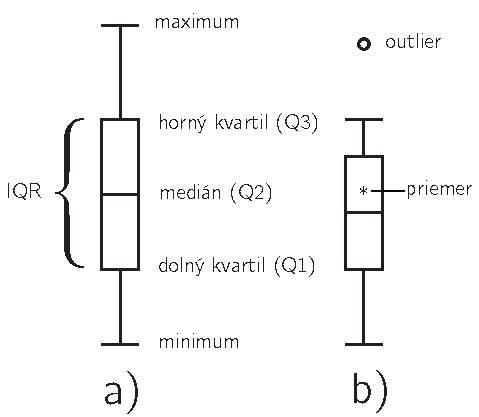
\includegraphics[width = 3.5in]{boxplot}
	\caption{Pôvodný návrh krabicového diagramu, ako bol prezentovaný v práci \textit{Exploratory Data Analysis}(1977) \cite{Tukey} }
	\label{fig:boxplot}
\end{figure}


\subsection{Ďalšie variácie krabicového diagramu}

Popularita krabicového diagramu nevyhnutne viedla k jeho vývoji a modifikáciám. Môžeme hovoriť o dvoch druhoch modifikácií. Jednak \textit{syntaktickej} (vizuálnej), kedy sa zachovávajú všetky vlastnosti a informácie ako v pôvodnom diagrame, len sa menia vizuálne prvky grafu. A modifikácii \textit{sémantickej} pridaním ďalšej popisnej informácie do grafu, čo má na záver vplyv aj na jeho vizuálnu stránku.


\begin{figure}
	\centering
	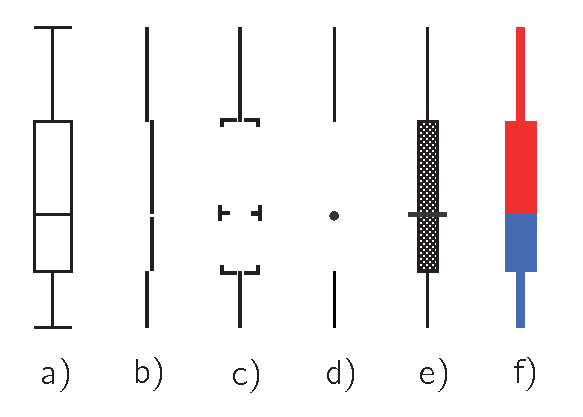
\includegraphics[width = 4in]{boxplot2}
	\caption{ a) Klasický krabicový diagram  b-f) Vizuálne variácie krabicového diagramu \mbox{b-c) 2 variácie pre kvartilový graf \cite{Tufte83}} \mbox{c) Skrátený krabicový diagram \cite{VisualSummaryPotter}} \mbox{e) \mbox{Range-bar} chart \cite{Spear}} \mbox{f) Farebná variácia \cite{Carr}}  }
	\label{fig:boxplotmodif1}
\end{figure}


\paragraph{}
{\large \textbf{\textit{N}}}a obrázkoch \ref{fig:boxplotmodif1} b-f) môžme vidieť niektoré vizuálne variácie krabicového diagramu. Vznik prvých troch motivovala snaha maximalizovať takzvaný \textit{data-ink} \cite{Tufte83}, teda množstvo atramentu alebo počet pixlov, ktoré zodpovedajú nejakým dátam. Autori sa teda snažili čo najviac znížiť počet vizuálnych prvkov a ponechať len tie, ktoré skutočne nesú nejakú informáciu. 

Na obrázku \ref{fig:boxplotmodif1} b) a c) vidíme dve z viacero riešení navrhnutých v knihe \textit{The Visual Display of Quantitative} \cite{Tufte83}, ktoré autor nazýva \textit{kvartilový graf}. Preceptuálne štúdie \cite{Stock} však ukázali, že tieto variácie sú výrazne menej presné ako originálny návrh.

Návrh d) ukazuje skrátený krabicový diagram \cite{VisualSummaryPotter}, ktorý sa taktiež snažil zredukovať množstvo okupovaného vizuálneho priestoru. Rozdielom je však to, že jeho účelom nie je existovať samostatne, ale ako súčasť \mbox{\textit{summary plot}-u}, ktorý zahŕňa histogram a ďalšie glify znázorňujúce informácie ako priemer, štandardná odchylka alebo koeficient asymetrie.

Obrázok \ref{fig:boxplotmodif1} e) znázorňuje predchodcu krabicového diagramu \textit{range} graf alebo tiež nazývaný \mbox{\textit{range-bar}} graf, ktorého autorkou je Mary Eleanor Spear \cite{Spear}.

Ako posledný príklad vizuálnej modifikácie uvádzame pridanie farieb do krabicového diagramu. Táto farebná variácia uchováva tvar diagramu, avšak časť nad mediánom je zafarbená inou farbou ako hodnoty pod. Autori článku odporúčajú červenú a modrú farbu, tak ako na obrázku \ref{fig:boxplotmodif1} f). Cieľom tohto prístupu bolo chápať krabicový diagram ako jednu percepčnú jednotku a nahradiť 5 symbolov jedným, čím sa mala znížiť námaha pozorovateľa pri analýze a taktiež uľahčiť porovnávanie viacerých diagramov navzájom. 

\begin{figure}
	\centering
	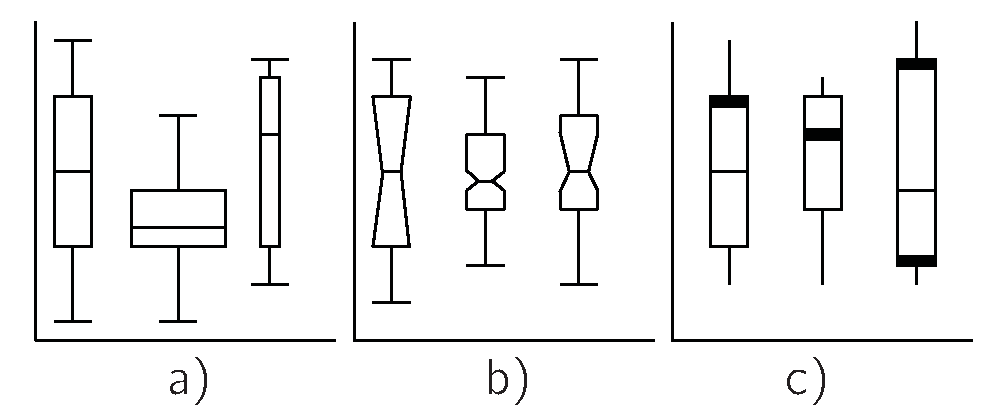
\includegraphics[width = 6in]{boxplot3}
	\caption{Krabicové diagramy s pridanou informáciou a) Krabicový diagram s variabilnou šírkou \cite{McGill} b) Vrúbkovaný krabicový diagram \cite{McGill} c) Krabicový diagram s informáciou o šikmosti dát \cite{Chamnein}}
	\label{fig:boxplotmodif2}
\end{figure}

\paragraph{}
{\large \textbf{\textit{K}}}rabicový diagram umožňuje svojim vzhľadom zakódovanie ďalšej informácie do grafu. Na obrázku \ref{fig:boxplotmodif2} vidíme aspoň niektoré najčastejšie úpravy krabicového diagramu, ktoré dopĺňajú dodatočnú informáciu zmenou parametrov vizuálnych prvkov krabicového diagramu.

Len rok po oficiálnom publikovaní krabicového diagramu vznikol článok \cite{McGill}, ktorý zhŕňa jeho tri najčastejšie používané modifikácie, z ktorých prvé dve môžme vidieť na obrázkoch \ref{fig:boxplotmodif2}a) a \ref{fig:boxplotmodif2}b) a tretí je ich kombináciou. V prvom prípade sa využíva šírka boxu na zakódovanie veľkosti množiny, ktorú skrýva za sebou diagram. Takýto graf sa nazýva \textit{Krabicový diagram s variabilnou šírkou}.  
V druhom prípade ide o takzvaný \textit{Vrúbkovaný krabicový diagram}. V tomto grafe sú pridané \textit{vrúbky}, ktoré zhruba naznačujú ako výrazné sú rozdiely v miere spoľahlivosti rôznych dátových množín. 

V niektorých prípadoch krabicový diagram zakrýva skutočný tvar dát, teda jeho šikmosť alebo modalitu, keďže jeho vzhľad nabáda k tomu, aby si užívateľ myslel, že sú dát zacentrované na stred a unimodálne. V práci s názvom \textit{Can the Box Plot be Improved?} \cite{Chamnein} autor uvádza príklad kedy skutočne rôznorodé dáta generujú rovnaký krabicový diagram. Tento problém rieši elegantným a čistým spôsobom pridaním hrubej čiary na základe koeficientu asymetrickosti $ \gamma $. Na obrázku \ref{fig:boxplotmodif2}c) môžme vidieť zľava asymetrické dáta, na stred zarovnané dáta a bimodálne dáta.

Krabicový diagram umožňuje mnoho ďalších rozšírení napríklad pridaním informácie o hustote dát (histogramový krabicový diagram, vázový diagram \cite{HistVasePlot} , huslový diagram \cite{ViolinPlot}), rozšírením pre viacrozmerné dáta (vrecový graf \cite{Bagplot}, 2D krabicový diagram \cite{Boxplot2D} ) alebo zobrazením hodnôt v inej súradnicovej sústave (napríklad polárnej - vejárový graf \cite{FanChart}). Opis týchto techník je však nad rámec tejto práce, preto ho tu ani nebudeme uvádzať.

\subsection{Úloha krabicového diagramu vo verifikácii}

Ako sme spomenuli v úvode tejto sekcie, vo všeobecnosti je úlohou krabicového diagramu zobraziť distribúciu dát v kompaktnom tvare a teda slúži na rýchle porovnanie distribúcií viacerých skupín dát.
Pri verifikácii predpovede spojitých premenných sa používa na viacero účelov a my tu spomenieme len niekoľko z nich. 

V prvom rade ide o porovnanie distribúcie predpovedí s distribúciou pozorovaní za istý časový interval. V takomto prípade máme vedľa seba iba dva krabicové diagramy, ktoré navzájom porovnávame. Použitie krabicového diagramu v takomto prípade, kedy jeden graf pozostáva iba z niekoľkých (2 až 4) krabicových diagramov považujeme za zbytočné. Pri takomto počte nie je potreba na redukciu vizuálnych prvkov a existujú lepšie techniky na vizualizáciu distribúcie, ktoré sprostredkúvajú viacej informácie a teda môže byť analýza efektívnejšia. 

Ďalším použitím je porovnanie distribúcie chýb predpovedí, či už pre rôzne merania, konkrétne predpovedané časy, rôzne predpovedné modely a podobne. Tu považujeme použitie krabicového diagramu za opodstatnené, keďže ide zväčša o porovnávanie väčšieho množstva distribúcií, a tak je potrebná jeho jednoduchosť, čitateľnosť, kompaktnosť a iné jeho vlastnosti.

\section{Histogram}
\label{sec:histogram}
Ďalším veľmi bežným spôsobom, ako vizualizovať distribúciu dát je pomocou \textit{histogramu}, ktorého existencia sa datuje do roku 1895, kedy ho uviedol vo svojej práci Karl Pearson \cite{histogram}. Histogram využíva veľmi jednoduchú myšlienku vizualizovať frekvencie hodnôt ako stĺpce rôznej výšky, ktorá sa v priebehu histórie analýzy dát ukázala ako veľmi užitočná.

\subsection{Konštrukcia histogramu}
Konštrukcia histogramu je pomerne jednoduchá. V prvom rade potrebujeme rozdeliť interval hodnôt na disjunktné podintervaly rovnakej dĺžky. Na vygenerovanie týchto intervalov využíva autor diagramu počiatok $ O $ a veľkosť intervalu $ w $. Prvý interval je $ \langle O, O + w) $ a všetky nasledujúce vzniknú posúvaním intervalu o dĺžku $ w $ v kladnom smere. Ďalej pre každý takto vzniknutý interval vypočítame koľko hodnôt doň spadá. Potom už môžme vykresliť jednotlivé stĺpce pre každý interval ako obdĺžniky so šírkou $ w $ a výškou, ktorá sa určí na základe početnosti hodnôt pre daný interval. Na obrázku \ref{fig:histogram} môžeme vidieť takýmto spôsobom vygenerovaný histogram.

\begin{figure}
	\centering
	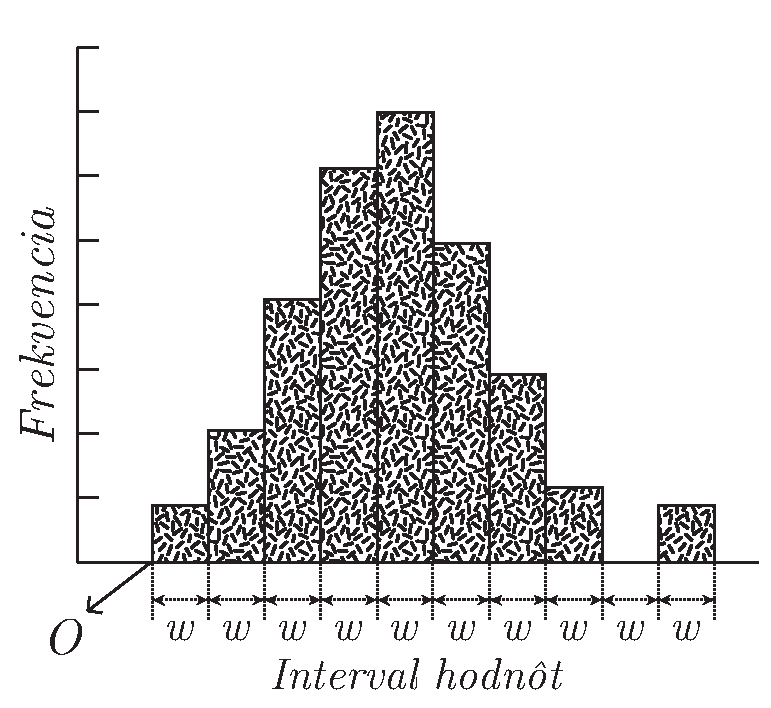
\includegraphics[width = 2.5in]{histogram}
	\caption{ Histogram }
	\label{fig:histogram}
\end{figure}

Z vyššie popísaného postupu a rovnako aj z obrázka \ref{fig:binsizehistogram} môžme vidieť, že konštrukcia histogramu závisí od zvoleného počiatku $ O $, no v prvom rade na zvolenej veľkosti intervalu $ w $. Z tohto dôvodu vzniklo mnoho prístupov, ktoré sa snažia optimalizovať $ w $, tak aby sa získal optimálny histogram. Optimálny histogram $ h(x) $ je taký, ktorý minimalizuje integrovanú strednú kvadratickú chybu (\textit{MISE}) vzhľadom na pôvodnú funkciu hustoty $ f(x) $. Túto chybu vypočítame takto: $ MISE = \int (h(x) - f(x))^2 dx $. 

Jedným z príkladov, ktorý toto využíva je algoritmus na generovanie optimálnej hodnoty $ w $, ktorý navrhol \textit{Shimazaki} a \textit{Shinomoto} \cite{OptBinSize}. Autori algoritmu požívajú dekompozíciu MISE na vytvorenie cenovej funkcie $ C_{n}(w) $ pre dĺžku intervalu $ w $:
\[
	C_{n}(w) = \frac{2\bar{k} - v}{(nw)^2}
\]
kde $ n $ je počet všetkých hodnôt množiny, $ \bar{k}$ je priemerný počet hodnôt v jednom intervale a $ v $ je variancia počtu hodnôt v intervaloch. Priebeh algoritmu je potom už len taký, že generuje postupne rôzne $ w $, kým nenájde také s najmenšou cenou $ C_{n}(w) $. 

\begin{figure}
	\centering
	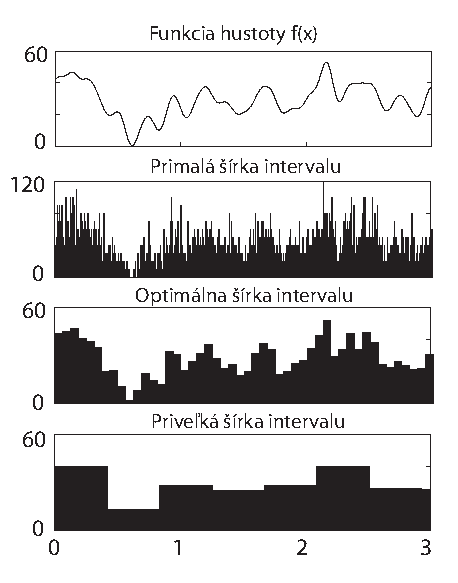
\includegraphics[width = 4in]{binsizehistogram}
	\caption{ Porovnanie rôznych dĺžok intervalov. Obrázok je upravený z pôvodného článku \cite{OptBinSize} }
	\label{fig:binsizehistogram}
\end{figure}

 
\subsection{Úloha histogramu vo verifikácii}
Ako sme už spomenuli, primárna úloha histogramu je detailná vizualizácia distribúcie dát. Vzhľadom k vysokej úrovni detailu, nie je jednoduché porovnávanie mnoho histogramov súčasne, tak ako to bolo u krabicového diagramu. Z tohto dôvodu sa zvyčajne v praxi porovnáva navzájom len niekoľko rôznych histogramov. Vo verifikácii histogramy slúžia na porovnanie distribúcie predpovedí a pozorovaní. Porovnávanie stĺpcov histogramov sa robí buď v dvoch rôznych diagramoch umiestnených vedľa seba alebo v jednom diagrame, kde sa k sebe prislúchajúce stĺpce umiestnia pri sebe a rozdielne zafarbia, aby ich bolo možné ľahšie rozlíšiť.

\section{Čiarový diagram}
\label{sec:linegraph}
\textit{Čiarový diagram} je najjednoduchší spôsob ako vizualizovať jednorozmerné dáta. Využíva sa najmä na vizualizáciu spojitej premennej, keďže čiara narozdiel od bodov podporuje vizuálny dojem spojitosti. Pôvod čiarového diagramu sa datuje do prapočiatkov vizualizácie informácií. Jeho autorom je zakladateľ grafických metód v štatistike William Playfair, ktorý objavil 4 typy diagramov medzi, ktorými bol aj čiarový diagram v roku 1786 \cite{HistoryOfInfoVis}.

\subsection{Konštrukcia čiarového diagramu}
Pri konštrukcii čiarového diagramu sa hodnoty z množiny zobrazia v karteziánskej sústave ako body a jednotlivé dvojice susedných bodov sa následne pospájajú čiarou. Na obrázku \ref{fig:linegraph} môžme vidieť príklad čiarového grafu vytvoreného týmto postupom.

Čiarový graf poskytuje rôznorodé úpravy, ktoré pridávajú ďalšiu informáciu do grafu alebo zlepšujú niektoré vizuálne vlastnosti. Napríklad je možné upravovať šírku, tvar alebo farbu čiary, pridávať ďalšie čiary do grafu, zvýrazniť jednotlivé body pre dané hodnoty, použiť iný typ interpolácie medzi bodmi (zvyčajne sa používa lineárna interpolácia) a podobne.

\subsection{Úloha čiarového diagramu vo verifikácii}
Vo verifikácii je účelom čiarového diagramu vizualizácia časových radov. Na \mbox{$ x $-ovej} osi zvykne byť časový interval s konkrétnymi dátumami predpovedí alebo hodiny predpovede. Rozdiel medzi nimi je ten, že konkrétny dátum je v histórii iba raz, zatiaľ čo model predpovedá pravidelne, takže predpovedné hodiny môžu byť rovnaké pre rôzne dátumy. Na \mbox{$ y $-ovej} osi teda bývajú buď jednotlivé hodnoty chýb alebo pre viacero hodnôt vypočítané štatistiky ako boli spomenuté v časti \ref{sec:errormeasurement}.
 

\begin{figure}
	\centering
	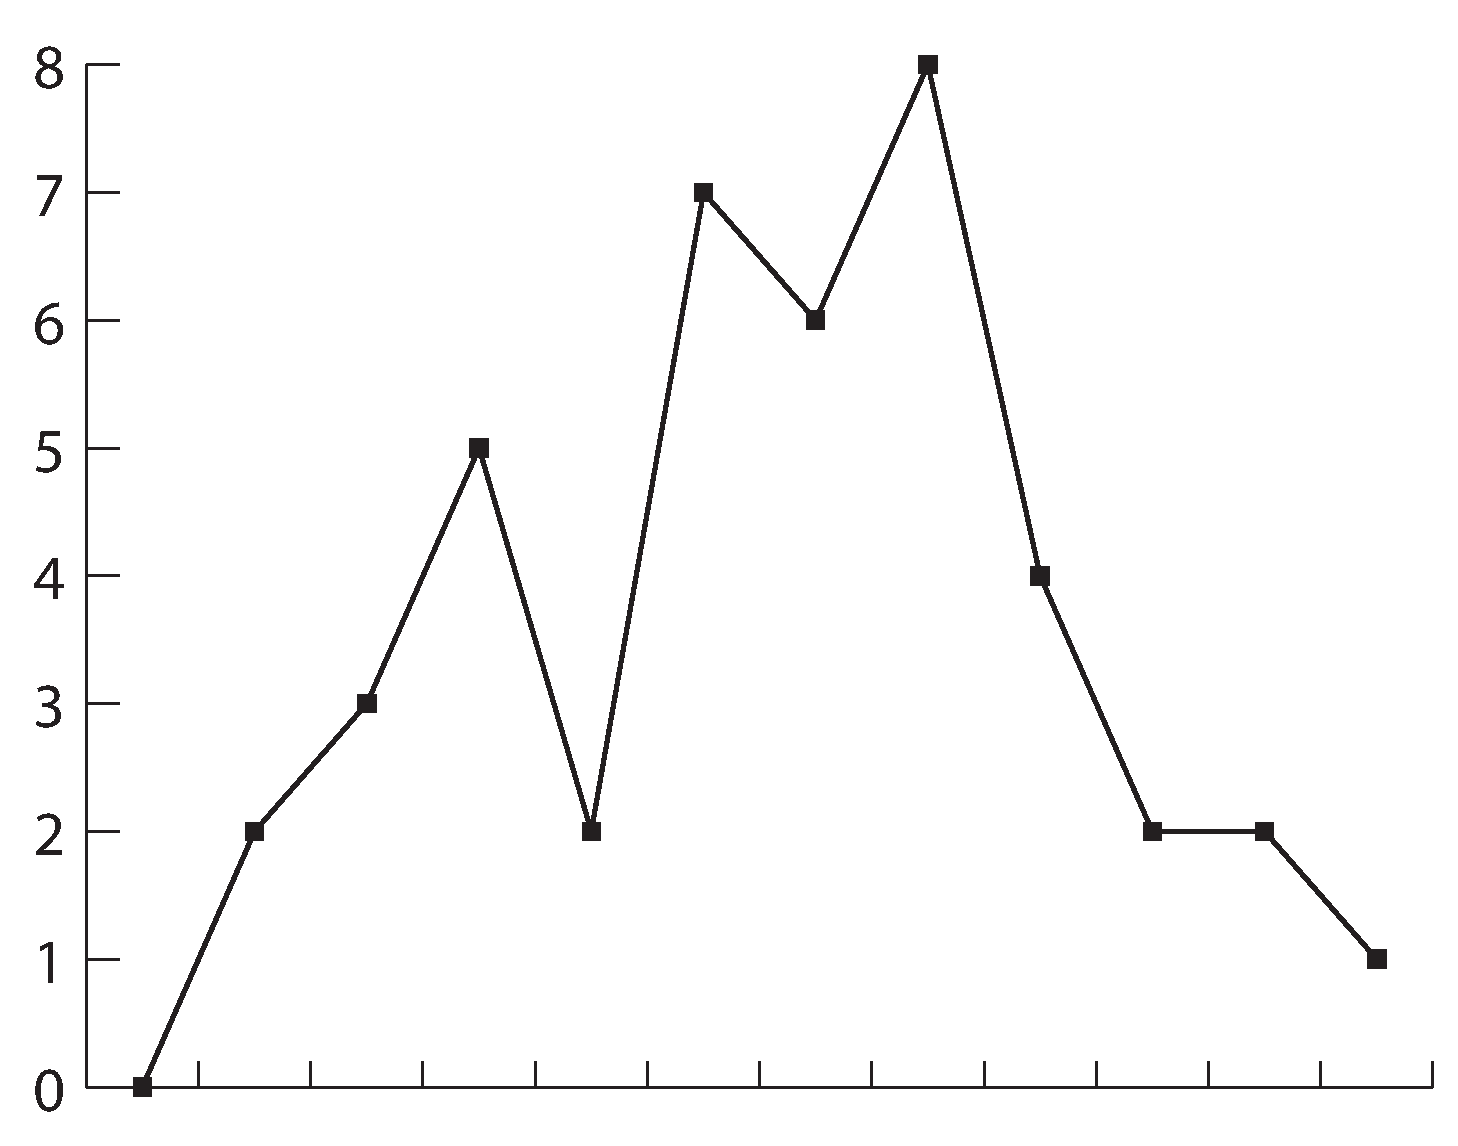
\includegraphics[width = 3in, height=1.5in]{linegraph}
	\caption{Príklad čiarového grafu vygenerovaného v programe Adobe Illustrator}
	\label{fig:linegraph}
\end{figure}

\section{Taylorov diagram}
\textit{Taylorov diagram} bol špeciálne navrhnutý pre verifikáciu modelov počasia, ktorého autorom je Karl. E. Taylor \cite{Taylor}. Podľa slov autora úlohou diagramu je štatistické zhrnutie, ako dobre si dátové vzory zodpovedajú v zmysle troch metrík: koeficient korelácie, strednej kvadratickej chyby a smerodajnej odchýlky. Použitie taylorovho diagramu nie je tak časté ako pri predchádzajúcich vizualizačných technikách, možno aj z dôvodu horšej čitateľnosti grafu a taktiež nemá takú veľkú tradíciu v štatistike, ako predošlé techniky. Podobnú snahu zobraziť tri štatistiky súčasne v jednom grafe mal aj Boer a Lambert vo svojom BLT diagrame \cite{Boer}. Tento typ grafu je veľmi podobný taylorovmu grafu, a keďže jeho použitie je ešte zriedkavejšie, tak sa mu v tejto práci nebudeme venovať.
  
\subsection{Konštrukcia taylorovho diagramu}
Taylorov graf porovnáva jednu alebo viacero dátových množín ($ f $) s jednou referenčnou množinou $ r $. Označme si hodnoty v porovnávanej množine $ f_{n} $ a s nimi spárované referenčné hodnoty $ r_{n} $, ktoré sú definované na $ N $ diskrétnych bodoch (napríklad v čase alebo priestore). Ako sme už spomenuli, taylorov graf vizualizuje 3 štatistiky súčasne, na čo využíva ich vzájomný geometrický vzťah. Týmito štatistikami sú: koeficient korelácie $ R $, centrovaná stredná kvadratická chyba $ E' $ a smerodajné odchýlky $ \sigma_{f} $ a $ \sigma_{r} $ pre $ f, r $.  Vzorce na výpočet sú nasledovné:
\[
	R = \dfrac{\frac{1}{N} \sum_{n=1}^{N}(f_{n} - \bar{f})(r_{n} - \bar{r})  }{\sigma_{f}\sigma_{r}}
\]
, kde $ \bar{f} $ a $ \bar{r} $ sú priemerné hodnoty daných množín.
\[
	E' = \sqrt{\frac{1}{N} \sum_{n=1}^{N}[(f_{n} - \bar{f}) - (r_{n} - \bar{r})]^2 }
\]
Pre pripomenutie chceme upozorniť, že nejde o strednú kvadratickú chybu, ktorá bola spomenutá v časti \ref{sec:errormeasurement}, ale o \textit{centrovanú} strednú kvadratickú chybu, ktorá je relatívna k stredu, teda priemeru skúmaných množín.

Rovnako pre $ \sigma_{f} $ aj $ \sigma_{r} $ je výpočet nasledovný:
\[
\sigma_{x} = \sqrt{\frac{1}{N} \sum_{n=1}^{N}[(x_{n} - \bar{x})]^2 }
\]

\begin{figure}
	\centering
	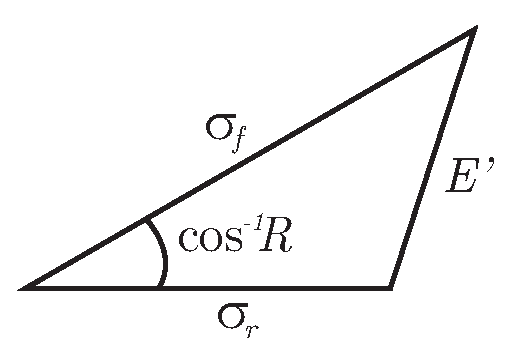
\includegraphics[width = 2.8in]{taylortriangle}
	\caption{ Geometrický vzťah pre popisné štatistiky $ R, E', \sigma_{r}, \sigma_{f} $ }
	\label{fig:gemrelationship}
\end{figure}

Kľúčovým bodom v konštrukcii diagramu je, že s využitím týchto troch respektíve štyroch štatistík môžme skonštruovať nasledovný vzťah:
\[
	E^{\prime2} = \sigma_{f}^{2} + \sigma_{r}^{2} - 2\sigma_{f}\sigma_{r}R
\]
, ktorý sa nápadne podobá na kosínusovú vetu:
\[
	a^{2} = b^{2} + c^{2} - 2bc\cos\alpha 
\]
, kde $ a, b $ a $ c $ sú dĺžky strán trojuholníka a uhol $ \alpha $ je protiľahlý uhol pre stranu $ a $. Geometrický vzťah pre $ R, E', \sigma_{f} $ a $ \sigma_{r} $ je zobrazený na obrázku \ref{fig:gemrelationship}. Ako vidíme na obrázku \ref{fig:taylordiagram}, jedna dátová množina sa pomocou týchto troch spomenutých hodnôt a vyššie uvedeného geometrického vzťahu zobrazí na grafe s polárnymi súradnicami. Azimutálna pozícia bodu nám hovorí o korelačnom koeficiente medzi množinami, preto sa vždy referenčný bod nachádza v najnižšej úrovni grafu, kde je korelácia rovná jednej. Vzdialenosť od počiatočného bodu $ 0 $ nám udáva smerodajnú odchýlku $ \sigma $ a vzdialenosť od referenčného bodu udáva centrovanú RMSE $ E' $. Pre jednoduchšie odčítavanie hodnôt sa pridávajú aj označené radiálne čiary jednak od bodu $ 0 $, ale aj od referenčného bodu, ktoré sa však v praxi zvyknú vynechávať.

\begin{figure}
	\centering
	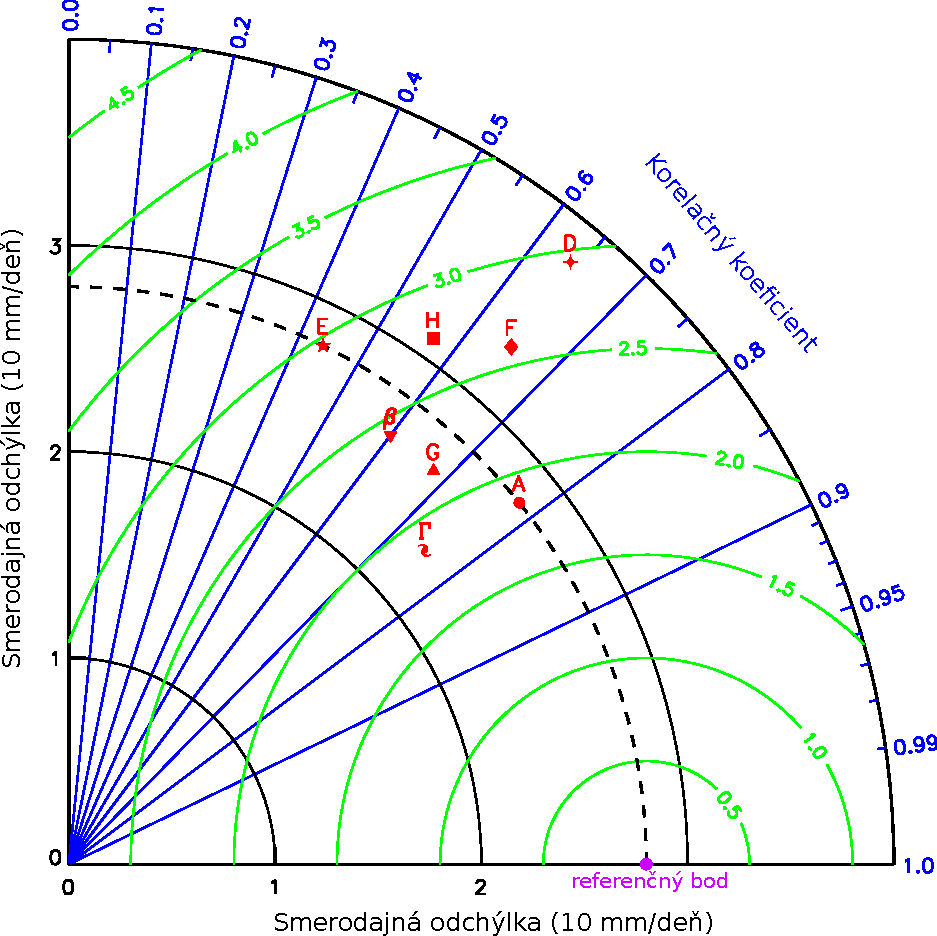
\includegraphics[width = 3.5in]{taylordiagram}
	\caption{ Taylorov diagram \cite{Taylor} }
	\label{fig:taylordiagram}
\end{figure}

Popísaným spôsobom vytvoríme základný taylorov diagram, ktorý však ponúka niekoľko modifikácií \cite{TaylorPrime}, z ktorých niektoré používané spomenieme:

\begin{singlespacing}
\begin{itemize} 
	\item Diagram môže byť rozšírený o ďalší kvadrant vľavo, na zobrazenie zápornej kolerácie 
	\item Štatistiky porovnávaných hodnôt môžu byť normalizované pomocou štatistík referenčných, čím dosiahneme, že na jednom diagrame možno zobraziť rôzne jednotky veličín.
	\item Izočiary sa vynechávajú, aby bolo možné lepšie vidieť zobrazené body.
	\item Pri porovnávaní výsledkov z viacerých verzií predpovedných modelov sa zvykne nakresliť šípka medzi týmito bodmi, aby bolo lepšie vidieť vzťah medzi nimi.
	\item Miera $ E' $ môže byť nahradená inou. Niektoré príklady mier možno nájsť v Taylorovom článku \cite{Taylor}
	\item Do grafu je možno pridať ďalšiu informáciu modifikovaním vizuálnych vlastností bodu podobne ako v bodovom diagrame. Jedným z príkladov je zobrazenie percentuálnej priemernej chyby pomocou rôznych symbolov.
\end{itemize}
\end{singlespacing}



\subsection{Úloha taylorovho diagramu vo verifikácii}
Tento typ diagramu bol priamo navrhnutý pre účely verifikácie predpovedných modelov počasia. Hlavným účelom diagramu je porovnávanie výkonu viacerých modelov alebo tiež jedného modelu s rôznymi nastaveniami parametrov. 

Taylorov diagram skrýva dáta pod komplikovaný matematický model, ktorý nám poskytuje 3 vyššie popísané charakteristiky dát na vizualizáciu. Ak sa k tomu pridáva fakt, že diagram umožňuje iba jednu referenčnú dátovú množinu, tak použitie tohto diagramu je značne obmedzené. Využitím spomínaných troch charakteristík taktiež výrazne strácame pohľad na detail dát, ale na druhej strane nám to umožňuje jednoduché porovnávanie pomerne veľkých a komplikovaných množín na malo priestore. 

Ďalšou slabinou je, že charakteristika $ E' $ sa počíta ako centrované RMSE, ktoré je relatívne vzhľadom na stred teda priemernú hodnotu dátovej množiny. Tento fakt implikuje to, že centrované RMSE nemá jednu dôležitú vlasnosť, ktorú naopak klasické RMSE má. Touto vlastnosťou je, že čím je RMSE bližšie k nule, tým podobnejšie sú aj dátové množiny. Keďže štatistická charakteristika $ E' $ nemá túto vlastnosť, tak nám euklidovská vzdialenosť skúmaného bodu od referenčného nedáva dobrú informáciu o podobnosti dvoch množín a môže pôsobiť mylne.
\chapter{Návrh vizualizácie}
Wolfgang Aigner vo svojej knihe \textit{Visualization of Time-Oriented Data} tvrdí, že riešenie problému vizualizácie vyžaduje zodpovedanie troch otázok: 
\begin{easylist}
	# Čo je vizualizované? - Čas a dáta
	# Prečo je to vizualizované? - Požiadavky používateľov
	# Ako je to vizualizované? - Vizuálna reprezentácia \\
\end{easylist}
\noindent Táto kapitola by mala odpovedať na všetky tieto tri položené otázky. 

\section{Špecifikácia požiadaviek na vizualizáciu}

\subsection{Charakteristika dát}
V prvom rade nám do verifikácie vstupujú surové dáta, ktorými sú pozorovania a predpovede.\\
- Surove data\\
--- pozorovania \\
--- predpovede \\
- Spracovane data \\
--- chyby \\
--- statistiky \\
------------------\\
- Numericke \\
- Ordinalne \\
- Spojité \\
--------------------\\
- Casovo orientovane \\
--- Scale (Skala): diskretny cas \\
--- Scope (Rozsah): point-based aj interval-based \\
--- Arrangment (Usporiadanie) : linearny \\
--- Viewpoint (Nahliadanie): usporiadane \\
--- Granularity: single \\
--- Time primitives: moment \\
--- Determinancy (Determinovanost): determinovane \\ 
------------------\\



\section{Návrh vizualizácie štatistík verifikácie} 
Štatistiky verifikácie sú dáta v časových radoch. V sekcii \ref{sec:linegraph} sme uviedli, že bežne používaným a veľmi účinným spôsobom vizualizácie časových radov je čiarový diagram. V našej práci sme sa odrazili od tohto faktu a navrhli sme dva pohľady na dáta. Jednak je to prehľad jedného druhu štatistík pre danú premennú počas skúmaného intervalu a druhým pohľadom je detail jedného časového podintervalu s rôznymi štatistikami alebo premennými.

\subsection{Prehľad štatistík {\small(\textit{Farebná mapa})}}
\label{sec:colormap}
Ako sme spomenuli vyššie, na vizualizáciu časových radov sa bežne používa čiarový diagram. Z našej skúsenosti vieme, že táto technika nie je vhodná pre porovnávanie mnohých chronologicky usporiadaných radov súčasne. Problémom je, že ak umiestnime viacero radov do jedného grafu, tak strácame informáciu o chronologickom poradí. Ak však umiestnime rady do grafov jednotlivo, tak pre väčšie množstvo dát nebudeme mať dostatočne veľký priestor.

Zvolili sme preto pomerne jednoduché a účinné riešenie, zobraziť štatistiky na iný vizuálny parameter, konkrétne na farbu. Jednotlivé hodnoty sa teda v grafe zobrazia ako za tesne sebou umiestnené farebné obdĺžniky \footnote{Experimentovali sme taktiež s inými tvarmi (kruhy a obdĺžniky so zaoblenými hranami), ale aj s rôznymi veľkostami medzier medzi tvarmi. Použité nastavenie sa však ukázalo ako najvhodnejšie pri porovnávaní hodnôt vo vertikálnom aj horizontálnom smere.}, ktoré vytvoria jeden celistvý pás (pozri porovnanie s čiarovým diagramom na obrázku \ref{fig:colormap}a. Umiestnením takýto pásov pod seba vytvoríme farebnú mapu štatistík. Výslednú vizualizáciu možno vidieť na obrázku \ref{fig:colormap}b. 

V našej aplikácii sa tento spôsob vizualizácie použil v dvoch prípadoch. Prvým prípadom bolo zobrazenie mesačných štatistík, pre 48 hodinové predpovede. Teda sme mali 12 mesiacov v roku a pre každý mesiac 48 hodnôt, čo sa nám zobrazilo ako farebná mapa $ 12 \times 48 $ (pozri obrázok \ref{fig:colormap}b). Druhým prípadom bolo zobrazenie chýb pre konkrétne predpovede, ktorých mohlo byť variabilný počet podľa nastavení systému. Zvyčajne však išlo približne o 30 predpovedí pre každý mesiac.

\begin{figure}
	\centering
	\hspace*{-0.45in}
	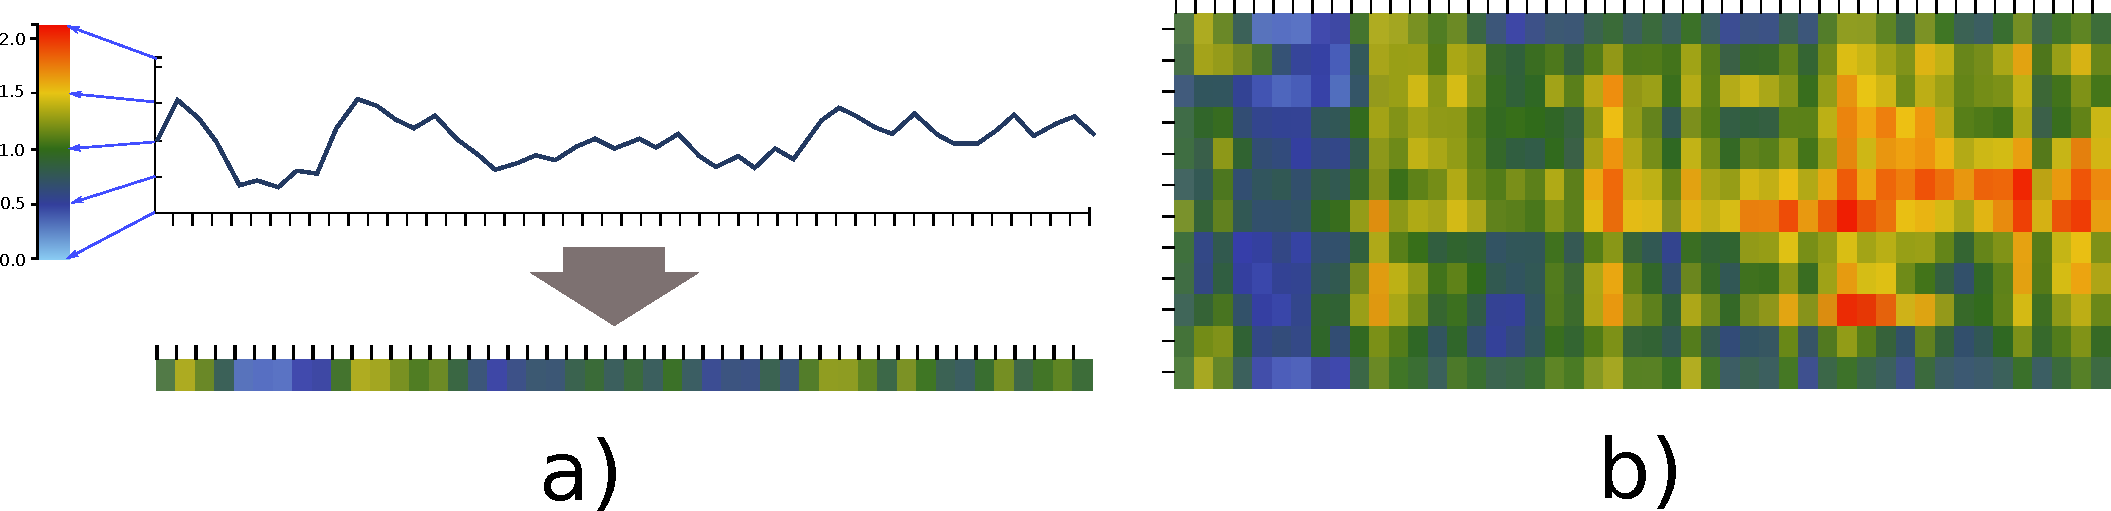
\includegraphics[width = 7.0in, height = 2.2in]{colormap}
	\caption{a) Konštrukcia jedného pásu zobrazením hodnôt grafu na farebnú škálu b) Výsledná vizualizácia, ako farebná mapa }
	\label{fig:colormap}
\end{figure}

\subsection{Detail štatistík {\small(\textit{Mnoho-čiarový diagram})}}
Napriek tomu, že zobrazením hodnôt na farbu nestrácame žiadnu informáciu, je dokázané, že človek nedokáže tak dobre porovnávať farby, ako napríklad vzdialenosti. Preto predošle spomenutá technika je síce vhodná na preskúmanie celého intervalu ako celku, avšak nie na detailné porovnávanie hodnôt v čase. Z tohto dôvodu sme sa rozhodli použiť taktiež spomínaný čiarový diagram. 

Tento typ diagramu poskytuje dostatočne veľký vizuálny priestor na to, aby sme doň mohli pridať ďalšie dáta. Rozhodli sme sa preto umožniť užívateľovi vizualizovať buď rôzne druhy štatistík súčasne pre danú predpoveď a veličinu (napr RMSE, MAE, MFE), alebo tiež rôzne veličiny (napr. tlak, teplotu, zrážky) pre túto predpoveď. V prvom prípade nám postačí jednotná škála, keďže sa hodnoty zväčša nachádzajú v podobnom rozmedzí. V druhom prípade je potrebných viacero škál, keďže napríklad chyby teploty sa pohybujú v rozmedzí 5 stupňov, tak chyby tlaku sa pohybujú v rozmedzí stoviek. Ak by sme tieto dve veličiny vizualizovali spolu, tak krivka teploty by bola sploštená natoľko, že by nebolo možné z nej odčítať hodnoty.

Vytvorenie mnoho-čiarového diagramu s jednotnou škálou je jednoduché, keďže sa na dizajne grafu nič nemení, len sa pridá ďalšia krivka. Pri viacerých rôznych škálach sa musia zobraziť aj tieto škály. Zvyčajne sa umiestňujú striedavo vľavo a vpravo, postupne za sebou smerom od stredu grafu. Problém však spočíva v tom, že pri väčšom počte nemôžme určiť, ktorá škála patrí ku ktorej krivke a s postupujúcou vzdialenosťou škály od grafu sa znižuje schopnosť užívateľa odčítavať hodnoty zo škály. V našej práci sme navrhli jednoduché spôsob, akým sme sa pokúsili vyriešiť oba problémy súčasne.

Naše riešenie spočíva v tom, že každá škála sa zobrazí ako obdĺžnik vyplnený farbou krivky, ktorá prislúcha k danej škále. Taktiež čiaročky indikujúce hodnoty v danom bode sa zobrazia pravidelne a v rovnakej vzdialenosti pre každú škálu.

Na obrázku \ref{fig:multilinegraph} môžme vidieť porovnanie bežne používaného spôsobu zobrazenia škál a nášho spôsobu. Náš spôsob jednoznačne priraďuje, pomocou farby, krivky ku škálam a jednotné, pravidelné rozmiestnenie indikátorov hodnôt nám rieši problém pri odčítavaní hodnôt, keďže nie je potrebné sa dívať na vzdialené škály.


\begin{figure}
	\centering
	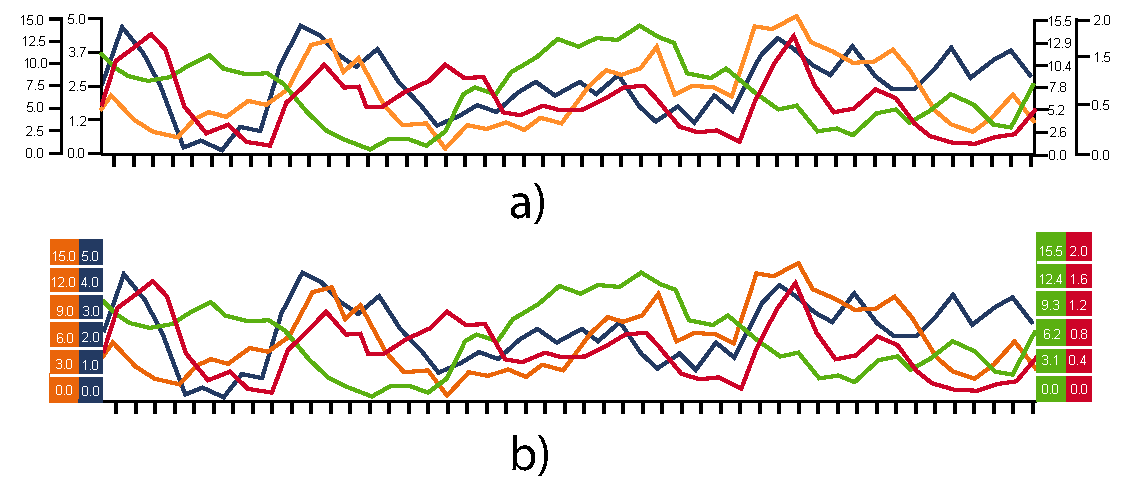
\includegraphics[width = 5in]{multilinegraph}
	\caption{a) Bežné zobrazenie viacerých škál b) Nami navrhnuté zobrazenie viacerých škál }
	\label{fig:multilinegraph} %TODO namiesto nul tam dat cisla
\end{figure}

\section{Návrh vizualizácie distribúcie chýb}
Pri verifikácii predpovede spojitej premennej sme použili štatistické metódy spomenuté v sekcii \ref{sec:errormeasurement}, ktorých výsledok sme následne vizualizovali. Pôvodné dáta však zostali skryté za použitým matematickým modelom, a tak sme stratili informáciu o distribúcii chyby. Pri verifikácii sa štandardne používajú tri metódy na priamu, či nepriamu vizualizáciu a analýzu distribúcie, ktoré sme opísali v kapitole \ref{chap:prevvis}. Týmito metódami sú bodový graf (pozri sekciu \ref{sec:scatterplot}), krabicový diagram (pozri sekciu \ref{sec:boxplot}) a histogram (pozri sekciu \ref{sec:histogram}).

My sme sa rozhodli napasovať vizualizáciu priamo na dáta verifikácie a pri jej návrhu sme vyskúšali niekoľko vizualizačných techník a zvážili ich silné a slabé stránky. 

\subsection{Graf hustoty} %Density plot

Jedným z viacerých spôsobov, ako pomerne presne určiť distribúciu chýb je pomocou \textit{grafu hustoty}. Ten sa skonštruuje jednoducho z \textit{funkcie hustoty}, ktorú získame \textit{odhadom hustoty} z dát. 

Prvý pohľad na dáta by nám vravel, že ide o dvojrozmerné dáta a teda je potrebné použiť odhad hustoty dvoch premenných. Takýto postup by samozrejme bol možný, ale doviedol by nás k chybnej vizualizácii a tak aj k mylnej predstave o dátach. Dôvodom je to, že máme záujem o analýzu distribúcie chýb pre každú hodinu predpovede zvlášť, čo znamená, že chcem zistiť distribúciu iba v jednom smere.

Pre vytvorenie grafu hustoty, v prvom rade je potrebné vybrať správny spôsob odhadu hustoty. Jedným z bežne používaným štandardným spôsobom je odhad hustoty pomocou jadra, po anglicky známy ako \textit{kernel density estimation} (KDE) [ref Rosenblatt 56, parzen 62].

Nech máme $ n $ hodnôt $ x_{i}, 1 \leq i \leq n $, z ktorých chceme určiť odhad hustoty, potom estimátor hustoty $ \hat{f}_h(x) $, ktorý aproximuje \textit{funkciu hustoty pravdepodobnosti} (PDF) $ f $, sa vypočíta takto:
\[
	\hat{f}_h(x) = \dfrac{1}{nh} \sum_{i=0}^{n}K\Big(\dfrac{x - x_{i}}{h}\Big)
\]
kde $ h $ je šírka jadra a $ K(x) $ je funkcia jadra (skrátene iba jadro), ktorá by mala spĺňať nasledovné vlastnosti:
\[  K(x) \geq 0 \]
\[  \int K(x) dx = 1 \]
tieto vlastnosti hovoria, že $ K(x) $ je na celom definičnom obore nezáporná a jej integrál je rovný 1, teda sa jedná o normalizovanú funkciu. Bolo preštudovaných mnoho jadier, ako napríklad uniformné, tri-angulárne, Epanechnikovo [29], kvadratické, Gaussové, kosínusové a veľa ďalších. Najbežnejšie a zrejme aj najpraktickejšie [18] je Gaussovo (normálne) jadro, ktoré sme použili aj my:
\[
	K(x) = \dfrac{1}{\sqrt{2\pi}}e^{-\frac{1}{2}x^2}
\]
Voľba jadra však nemá na výsledok až taký vplyv, ako voľba šírky jadra $ h $. My sme použili výpočet šírky jadra na základe dátovej množiny, ktorý aproximuje optimálnu šírku jadra [Scott 1992; Bowman and Azzalini 1997] \footnote{Optimálna šírka jadra je taká, ktorá minimalizuje \textit{strednú integrovanú kvadratickú chybu}.}. Všeobecne pre $ d $ dimenzionálne dáta je vzorec nasledovný:
\[
	h = \sigma \Big(\frac{4}{(d + 2)n}\Big)^{\frac{1}{d+4}}
\]
kde $ \sigma $ je smerodajná odchýlka vypočítaná z daných dát a $ n $ je veľkosť dátovej množiny. V našom prípade je $ d = 1 $, a tak sa nám vzorec zjednoduší na
\[
	h = \sigma \Big(\dfrac{4}{3n}\Big)^{\frac{1}{5}}
\] 
Aby sme zjednodušili výpočet, tak sme si konštanty vypočítali predom a zaokrúhlili na 2 desatinné miesta, čo považujeme za dostačujúce. Výsledný vzorec, ktorý sa nakoniec objavil v aplikácii je takýto:
\[
	h = 1.06 \times \sigma \times n^{-\frac{1}{5}}
\]

Takýmto spôsobom sme si pre každú hodinu predpovede určili samostatnú funkciu $ \hat{f}_{h}(x) $, ktorú môžme vizualizovať. Zvyčajne sa funkcie hustoty vizualizujú ako bežné funkcie, teda pomocou čiarového diagramu, tak ako na obrázku \ref{fig:XY}. V našom prípade by bol tento prístup nepraktický, keďže máme veľké množstvo funkcií, tak jednak by bola takáto vizualizácia nepraktická pri porovnávaní distribúcií a taktiež na to nemáme potrebný vizuálny priestor.

Opäť sme teda zvolili štandardné riešenie, ako ušetriť vzácny priestor a to tak, že hodnoty, ktoré by boli zobrazené na $ y $-ovú os zobrazíme na zvolenú farebnú škálu. Vďaka tomu by teoreticky mohol mať graf hustoty pre jeden čas predpovede šírku 1 pixel bez straty akejkoľvek informácie.

Vieme, že pre ľudí nie je také jednoduché pozorovať malé rozdiely medzi dvoma farbami. Testovaním sme zistili, že tento fakt spôsobuje problémy aj pri našej vizualizácii, kedy sa pre pozorovateľa strácajú jemné výkyvy hodnôt. Riešením by bolo nepoužiť spojité, ale diskrétne farbenie, ktoré je rozdeľuje interval hodnôt na podintervaly, ku ktorým priradí konkrétnu farbu (pozri obr. \ref{fig:XYZ}). Výhodu je, že takéto farbenie má výraznejšie farebné rozdiely. Týmto spôsobom by sme však stratili priveľa informácie a nebolo by potrebné použiť na odhad hustoty KDE, ale postačoval by aj histogram. 

Riešenie tohto problému sme našli v práci od Takafumi Saita z roku 2005 \cite{Saito}. V tomto článku autor so svojimi kolegami navrhuje nový spôsob pseudo farbenia, ktoré nazýva \textit{two-tone pseudo coloring} alebo inak po slovensky \textit{dvojtónové pseudo farbenie}. Navrhnutá metóda priraďuje každej hodnote intervalu dve výrazne rôzne farby resp. farebné časti. Toto sa uskutočňuje podobne ako pri spojitom farbení, avšak sa neinterpolujú farby, ale pomer veľkostí dvoch zafarbených častí. Na obrázku \ref{fig:twotone} možno vidieť porovnanie troch spomenutých techník farbenia.

\begin{figure}
	\centering
	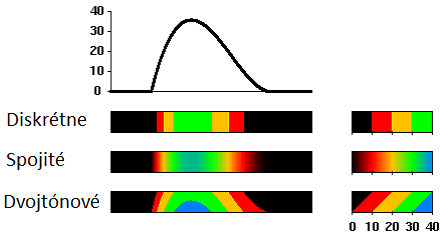
\includegraphics[width = 3.5in]{twotone}
	\caption{Porovnanie dvoch konvenčných techník farbenia so Saitovým dvojtónovým farbením. Obrázok pochádza z pôvodného článku \cite{Saito}. }
	\label{fig:twotone} 
\end{figure}

%TODO Ďalší problém - nevidno hranice!. 

Na obrázku \ref{fig:XYZ} vodno porovnanie vizualizácií s použitím spojitého a dvojtónového farbenia.

\subsection{Pruhový kvantilový diagram} 
Z časti \ref{subsec:scatterplot} sme už dobre oboznámený s pojmom kvantil. Klasický kvantilový diagram [ref] zobrazuje kvantil hodnôt pre jednu dimenziu. Ak si vezmeme naše dáta, kde pre každý čas je niekoľko chýb predpovedí, tak kvantilový diagram skonštruujeme tak, že pre každý čas vypočítame kvantil, ktorý zobrazíme ako bod alebo ako súčasť lomenej čiary v grafe.
Prirodzeným rozšírením je zobrazovať nielen jeden kvantil, ale mnoho kvantilov súčasne. Zvyčajne sú to tieto kvantily $ Q_{0.02}, Q_{0.98}, Q_{0.25}, Q_{0.75}, Q_{0.5} $. V našej práci sme využili toto rozšírenie na lepšie zobrazenie distribúcie a navrhli sme takzvaný \textit{pruhový kvantilový diagram}.

Jeden \textit{pruh} v grafe definujeme pomocou dvojíc hodnôt v čase - spodným a jeho protiľahlým kvantilom. Spodným kvantilom je kvantil $ Q_{\alpha} $ a k nemu protiľahlý je kvantil $ Q_{1 - \alpha} $, kde $ 0 \leq \alpha \leq \frac{1}{2} $. Vidíme teda, že pruh ohraničuje hodnoty v okolí stredu usporiadanej množiny dát. Špeciálnym prípadom pruhu je pre $ \alpha = \frac{1}{2} $, vtedy spodný aj horný kvantil je $ Q_{0.5} $, čo je vlastne medián.

Pri návrhu vizualizácie sme sa snažili, aby mohol mať diagram variabilný počet pruhov a taktiež, aby rozostup medzi pruhmi bol pravidelný. Pri riešení tohto problému, sme sa inšpirovali krabicovým diagramom, kde sa hodnoty delia mediánom na dve časti, ktoré sa ďalej taktiež delia ich mediánom. Ide teda o rekurzívne delenie usporiadanej množiny na polovicu do hĺbky 2. Túto myšlienku sme rozšírili na ľubovoľnú hĺbku delenia $ d $. Potom $ i $-ty pruh $ \mathcal{P}_{d}(i) $ pre hĺbku $ d $ definujeme takto:
\[
	p_{d}(i) = (Q_{\alpha},Q_{1 - \alpha}) , \alpha = i \times (0.5)^d 	
\]
\[
	\mathcal{P}_{d}(i) = \{ (t,p_{d}(i)) : t \in I \}
\]
a množina všetkých pruhov grafu pre hĺbku delenia $ d $ je definovaná takto:
\[
	\{ \mathcal{P}_{d}(i) : 0 \leq i \leq 2^{d-1} , i \in \mathbb{N} \}
\]
Aby sme sa vyhli rekruzii, vypočítali sme si krok medzi susednými kvantilmi pri hĺbke $ d $, ktorý je $ (0.5)^d $, a jednotlivé pruhy sme generovali s týmto krokom. Pri rekruzívnom delení sa vygeneruje $ 2^d $ kvantilov a z nich je možné vyrobiť $ 2^{d - 1} $ pruhov, preto sme index $ i $ obmedzili na $ i \leq 2^{d-1} $. Z tohto vidíme, že počet pruhov grafe s rastúcou hĺbkou rastie exponenciálne, preto odporúčame, aby $ d $ bolo maximálne 4, kedy sa nám množina rozdelí na 16 častí 15 hexadecilmi a tak vznikne 8 pruhov.

% TODO obrázok 
Na obrázku \ref{fig:pruh} vidíme, že takto definovaný pruh sa potom vizualizuje, ako plocha medzi krivkami, ktoré tvoria dvojice hodnôt patriace danému pruhu, s výnimkou špeciálneho prípadu $ Q_{0.5} $, ktorý vizualizujeme ako krivku.



%TODO toto musím ešte celé premyslieť!


\subsection{Funkčný krabicový diagram}
Pre pochopenie dát je dôležité, aby sme sa vedeli pozrieť na hodnoty v ich kontexte. Všetky predošlé techniky uvažovali o chybe ako o samostatnej hodnote pre určitý predpovedný čas, avšak chyby sa nenachádzajú len v kontexte predpovedného času, ale aj v kontexte konkrétnej predpovede. Preto môžme uvažovať o predpovediach ako o funkciách $ x_{i}(t) $, kde $ i \in \{1..n\}$ je poradie predpovede a $ t \in I $ je čas predpovede, kde $ I $ je časový interval predpovede z $ \mathbb{R} $ (v našom prípade sa jednalo o dvojdňovú, teda 48 hodinovú predpoveď).

Takýmto spôsobom sme sa dostali do novej situácie, kedy nechceme vizualizovať distribúciu jednotlivých chýb, ale celých predpovedí, ktoré chápeme ako funkcie. Na riešenie tohto problému existuje niekoľko spôsobov, z ktorých sme si zvolili \textit{funkčný krabicový diagram} \cite{FunctionalBoxplot}, keďže myšlienkovo vychádza z klasického krabicového diagramu, ktorý je jednak na túto situáciu vhodný ale je tiež medzi užívateľmi dobre známy a zaužívaný.

Ako sme spomenuli v časti \ref{subsec:boxplot}, klasický krabicový diagram potrebuje na svoju konštrukciu 5 hodnôt: 3 kvartily a 2 extrémy. Aby sme tieto hodnoty našli pre funkcie, musíme ich vedieť porovnať a povedať, ktorá je \textquotedblleft väčšia\textquotedblright alebo \textquotedblleft menšia\textquotedblright. Autori funkčného krabicového diagramu riešia problém s využitím takzvanej pásmovej hĺbky (\textit{band depth}) \cite{BandDepth}. Grafom $ G $ funkcie $ x $ je množina bodov $ G = \{ (t,x(t)) : t \in I \} $. Pásmo $ \mathcal{B} $ (\textit{band}) v $ \mathbb{R}^{2}  $ ohraničené krivkami $ x_{i_{1}}, x_{i_{2}}, .. , x_{i_{k}} $, kde $ k \geq 2 $ je definované takto:
\[
	\mathcal{B}(x_{i_{1}}, x_{i_{2}}, .. , x_{i_{k}}) = \{ (t,y) : t \in I, \min_{r=1..k}x_{i_{r}}(t) \leq y \leq \min_{r=1..k}x_{i_{r}}(t) \}
\]
Pásmo $ \mathcal{B} $ je teda množina všetkých bodov existujúcich medzi extrémami všetkých kriviek, ktoré doň vstupujú ako parameter. 
Pomocou týchto dvoch funkcií môžme definovať pomocnú funkciu $ BD_{n}^{(j)}(x) $ pre krivku $ x $, ktorá vyzerá takto:
\[
	BD^{(j)}_{n}(x) = {n \choose j}^{-1} \sum_{1 \leq i_{1} < i_{2} < ... < i_{j} \leq n} \mathcal{I}\{ G(x) \subset \mathcal{B}(x_{i_{1}}, ... ,x_{i_{j}}) \}, j \geq 2
\]
kde $ j $ je počet kriviek definujúce pásmo $ \mathcal{B} $, $ n $ je celkový počet kriviek a $ \mathcal{I} $ je takáto funkcia:
\[
	\mathcal{I}(x) = \left\{
	\begin{array}{ll}
	1 & \mbox{ak platí x}  \\
	0 & \mbox{ak neplatí x} 
	\end{array}
	\right.
\]
Pomocná funkcia $ BD $ pre krivku $ x $ definuje pomer všetkých pásem zložených z $ j $ kriviek, v ktorých sa graf $ G(x) $ nachádza, ku všetkým možným $ j $-ticiam kriviek vybraným z $ n $. 
Samotná funkcia pásmovej hĺbky $ \mathcal{BD} $ pre krivku $ x $ je definovaná takto:
\[
	\mathcal{BD}_{n, J}(x) = \sum_{j = 2}^{J} BD^{(j)}_{n}(x), J \geq 2
\]
Hĺbka pásma $ \mathcal{BD} $ je teda suma všetkých $ BD $ pre počet kriviek 2 až $ J $.

Autor článku definujúci pojem pásmová hĺbka navrhol taktiež flexibilnejšiu verziu s použitím pomocnej funkcie $ MBD $ (\textit{modified band depth}) \cite{BandDepth}. V pravom rade je potrebné zadefinovať si funkciu $ A $, ktorá určí všetky časové body, kedy sa krivka $ x $ nachádza v pásme $ B $.
\[
	A(x, B) = \{ t \in I : (t, x(t)) \in G(x) \wedge (t, x(t)) \in B \}
\]
V spomínanom článku autori využívajú alternatívnu definíciu funkcie $ A $, do ktorej vstupuje $ j + 1 $ kriviek. Jej význam zostáva rovnaký ako pri našej definícii, avšak náš prístup považujeme za jednoduchší a zrozumiteľnejší. S využitím \textit{Lebesguevoej miery} $ \lambda $ autori ďalej definujú funkciu $ \lambda_{r} $, ktorá nám dáva "pomer času, ktorý krivka strávi v pásme":
\[
	\lambda_{r}(A) = \dfrac{\lambda(A)}{\lambda(I)} 
\]
Nová pomocná funkcia $ MBD $ je definovaná nasledovne:
\[
	MBD^{(j)}_{n}(x) = {n \choose j}^{-1} \sum_{1 \leq i_{1} < i_{2} < ... < i_{j} \leq n} \lambda_{r}\{ A(x, \mathcal{B}(x_{i_{1}}, ... ,x_{i_{j}})) \}, j \geq 2
\]
Ak platí, že $ G(x) \subset \mathcal{B}(x_{i_{1}}, ... ,x_{i_{j}}) $, tak funkcia $ MBD $ sa degeneruje na $ BD $ \cite{FunctionalBoxplot}.

V našej aplikácii sme sa rozhodli, že budeme pásmo definovať pomocou iba dvoch kriviek, čo nám vzorec výrazne zjednodušilo. Taktiež to implikovalo fakt, že pri výpočte $ MBD $ nie je potrebné $ {n \choose j}^{-1} $, keďže berieme pásma zložené vždy z rovnakého počtu kriviek. Pre naše účely sme si taktiež zjednodušili funkciu $ \lambda_{r} $ na $ \lambda $, keďže nepotrebujeme vlastnosť tejto funkcie, ktorá dosahovala to, že $ MBD $ pre špeciálny prípad degeneruje na $ BD $. Po týchto úpravách výsledný vzorec pre naše $ \mathcal{BD}' $ vyzerá nasledovne:
\[
	\mathcal{BD}'_{n}(x) = \sum_{1 \leq i_{1} < i_{2} \leq n} \lambda\{ A(x, \mathcal{B}(x_{i_{1}},x_{i_{2}})) \}
\]
Teraz, keď sme úspešne definovali mieru, podľa ktorej môžme usporiadať funkcie resp. ich krivky, je veľmi ľahké skonštruovať funkčný krabicový diagram.

\paragraph{}
Nech sú naše funkcie predpovedí $ x_{1},.., x_{n} $ usporiadané zostupne podľa $ \mathcal{BD}' $. Potom krivka pre funkciu $ x_{1} $ má najvyššiu pásmovú hĺbku a predstavuje strednú hodnotu pre množinu funkcií, teda niečo podobné ako medián hodnôt pri krabicovom diagrame. Pri konštrukcii funkcionálneho diagramu nám taktiež pomôže koncept centrálneho regiónu \cite{Liu}. Centrálny región $ C $ pre 50\% kriviek je pásmo vytvorené z 50\% najhlbších kriviek, teda:
\[
	C_{0.5} = B(x_{1}, x_{2}, .., x_{\lceil n / 2 \rceil} )
\] 
Vidíme, že Centrálny región $ C_{0.5} $ zaobaľuje 50\% najhlbších kriviek, a teda sa jedná o akúsi analógiu pre medzikvartálový rozsah (IQR) v klasickom krabicovom diagrame (pozri sekciu \ref{subsec:boxplot}), ktorý ohraničoval 50\% centrálnych dát. Zobrazením hraničných bodov tohto regiónu získame obálku myšlienkovo totožnú boxu v krabicovom diagrame (pozri obrázok \ref{fig:functionalboxplot}b) ). Táto myšlienka sa dá použiť ďalej a môžme, tak ako na obrázku \ref{fig:functionalboxplot}c) , zobraziť taktiež 25\%-ný a 75\%-ný centrálny región $ C_{0.25} $, $ C_{0.75} $, avšak kvôli nižšej čitateľnosti grafu sme túto alternatívu nepoužili.

V prípade, že nepotrebujeme identifikovať \textit{outlier}-ov, tak extremálne hodnoty je už veľmi jednoduché získať, pretože ich tvorí pásmo zložené zo všetkých kriviek $ B(x_{1}, .., x_{n}) $. V opačnom prípade musíme najprv identifikovať \textit{outlier}-ov, ktorých potom vylúčime z výpočtov. Opäť sa využíva myšlienka z klasického krabicového diagramu, kedy sa \textit{outlier} určil pomocou hodnoty $ c \times IQR $, kde $ c $ bolo zvyčajne 1.5. Hranice sa teda získajú naškálovaním centrálneho regiónu so škálovacím faktorom 1.5 a všetky krivky, ktoré sa v tomto regióne nenachádzajú, budú považované za \textit{outlier}-ov. Test na \textit{outlier}-a vyzerá teda takto:
\[	y_{i}(t) = 1.5 \times x_{i}(t) \]
\[	isOutlier(x) = [ G(x) \nsubseteq B(y_{1},..,y_{\lceil n / 2 \rceil}) ] \]
Na obrázku \ref{fig:functionalboxplot}b) môžme vidieť červené prerušované čiary, ktorými sú \textit{outlier}-i znázornené.

V našej práci sme do diagramu pridali ešte jednu krivku pre ľubovoľnú štatistiku vypočítanú z chýb ako napríklad MFE, MAE alebo RMSE (pozri sekciu \ref{sec:errormeasurement}). Takto môžme spraviť porovnanie distribúcie chýb s vypočítanou štatistikou.
%TODO to je troška klamstvo ne?


\begin{figure}
	\centering
	\hspace*{-0.9in}
	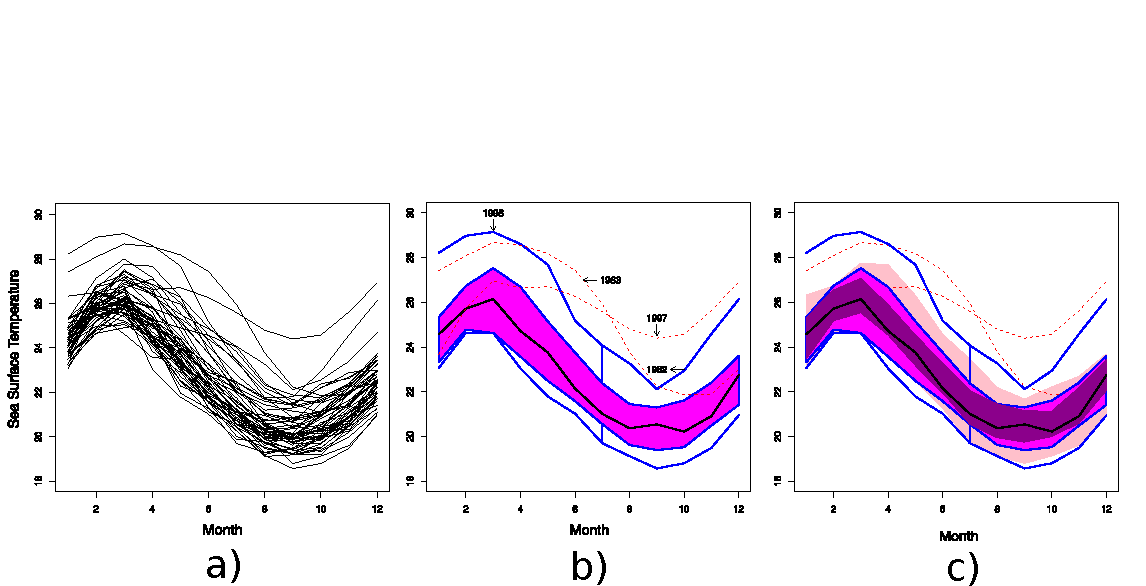
\includegraphics[width = 7.5in]{functionalboxplot}
	\caption{Obrázky z článku \textit{Functional Boxplots}  \cite{FunctionalBoxplot}  a) Funkcie meraní teploty hladiny mora b) Funkčný krabicový diagram c) Rozšírený Funkčný krabicový diagram o centrálne regióny $ C_{0.25} $ a $ C_{0.75} $ }
	\label{fig:functionalboxplot}
\end{figure}
%TODO tento obrazok skresat zhora a tak

%TODO obrazok pasmo

\subsection{Distribucia za cely rok} %TODO lepsie pomenovat - tuto bude navrh pre distribuciu chyb pomocou standrard deviation a urobi sa kruzok danej velkosti


\subsection{Porovnanie metód}

Tu bude pekný obrázok a obkeci. \\
Graf hustoty je presnejsi, ale menej citatelny. \\
Pruhovy kvantilovy diagram nahradzuje krabicovy diagram. \\
Funkcionalny krabicovy riesi distribuciu funkcii.


\section{Návrh farebnej palety}
Farba je pravdepodobne najviac podceňovaný a nesprávne používaný vizuálny parameter vo vizualizácii dát. V tejto časti opisujeme návrh farebnej palety pre jednotlivé vyššie spomenuté vizualizačné techniky.

% Asi len pre farebnú mapu sa rozpíšem a pre ostatné, to iba rýchlo zhrnem

\subsection{Farebná mapa}
Návrhu farebnej palety pre farebnú mapu sme venovali zvýšenú pozornosť, keďže farba hrá pri tomto type vizualizácie najpodstatnejšiu úlohu.

V prvom momente sme siahli po veľmi prvoplánovom riešení a použili sme takzvanú \textit{dúhovú farebnú škálu}, ktorú možno vidieť v sekcii \ref{sec:colormap} na obrázku \ref{fig:colormap}. Výskum ukázal a mnohý vedci sa na tom zhodujú, že tento typ farebnej palety je len zriedkakedy najlepšia voľba pri vizualizácii. Dúhové farebné palety majú niekoľko slabých stránok, ktoré zhŕňa Theresa-Marie Rhyne vo svojom článku \cite{Rhyne}.
%TODO sem napisem par slabych stranok

Z tohto dôvodu sme sa rozhodli použiť prechod medzi troma farbami: červenou, bielou a modrou. Červená znázorňuje kladné maximum, biela hodnoty blízko nuly a modrá záporné maximum. Výber týchto troch farieb bol jednoduchý ... 

%TODO napapisat z akej stranky to je vlastne tie fraby

- monochrome cez 3 farby \\
- monochrome 2 farby ostro rozdelene \\
- ekvalizacia histogramom / boxplotom \\
\subsection{Mnoho-čiarový diagram}
- pri stats to je jedno \\
- pri progress sme zvyraznili klzavy priemer 

\subsection{Graf hustoty}
 - monochrome 
\subsection{Pruhový diagram}

\subsection{Funkčný krabicový diagram}

\section{Návrh rozloženia prvkov vizualizácie}
Výsledná obrazovka systému sa nebude skladať iba z jedného typu vizualizácie, ale z viacerých grafov a iných častí, ktoré spolu užívateľovi vytvoria dostatočne dobrú predstavu o dátach. Tieto časti budeme nazývať prvky alebo komponenty vizualizácie. Jednotlivým prvkom sme dali nasledovné pomenovania: 

\begin{itemize}
	\item\textit{Meta informácie} je tabuľka obsahujúca informácie o stanici (Názov, geografická poloha, nadmorská výška), názov modelu, interval verifikácie, spôsob interpolácie a podobne.  
		
	\item\textit{Prehľad} je komponent vizualizácie, ktorý by mal poskytovať celistvý pohľad na všetky mesačné štatistiky. Jeho úlohou nie je detailné zobrazenie chýb, ale odhalenie vzorov, trendov a výkyvov vo fungovaní modelu počas skúmaného intervalu.
	
	\item\textit{Zjednodušený prehľad} je vo svojej podstate rovnaký ako \textit{Prehľad}. Rozdielom je však menšia plocha, ktorú zaberá, zjednodušená farebná škála a chýbajúce popisky.
	
	\item\textit{Celkový priebeh} zobrazuje priebeh chýb počas celého intervalu. Nie však z pohľadu 48 predpovedných hodín (ako \textit{Prehľad}), ale z pohľadu jednotlivých dní.
	
	\item\textit{Detail štatistík} je prvok slúžiaci na detailnejšie skúmanie štatistík počas jedného mesiaca. V grafe sa nachádzajú všetky dostupné štatistiky pre daný mesiac.
	
	\item\textit{Detail chýb} pre daný mesiac, nám dáva pohľad na chyby predpovede, z ktorých sa počítali štatistiky.
	
	\item\textit{Distribúcia chýb} sa taktiež zobrazuje pre konkrétny mesiac a týmto komponentom je graf, v ktorom je zobrazená distribúcia chýb v danom mesiaci.
\end{itemize}

 Pre lepšiu orientáciu v kapitole sme pre jednotlivé prvky priradili aj obrázkové ikony. Jednotlivé priradenia sú vyobrazené na obrázku \ref{fig:designicons}. 
 
 Pri návrhu rozloženie prvkov vizualizácie na obrazovke sme sa rozhodovali medzi dvoma smermi uvažovania, ktoré opíšeme v tejto sekcii. 

\begin{figure}
	\centering
	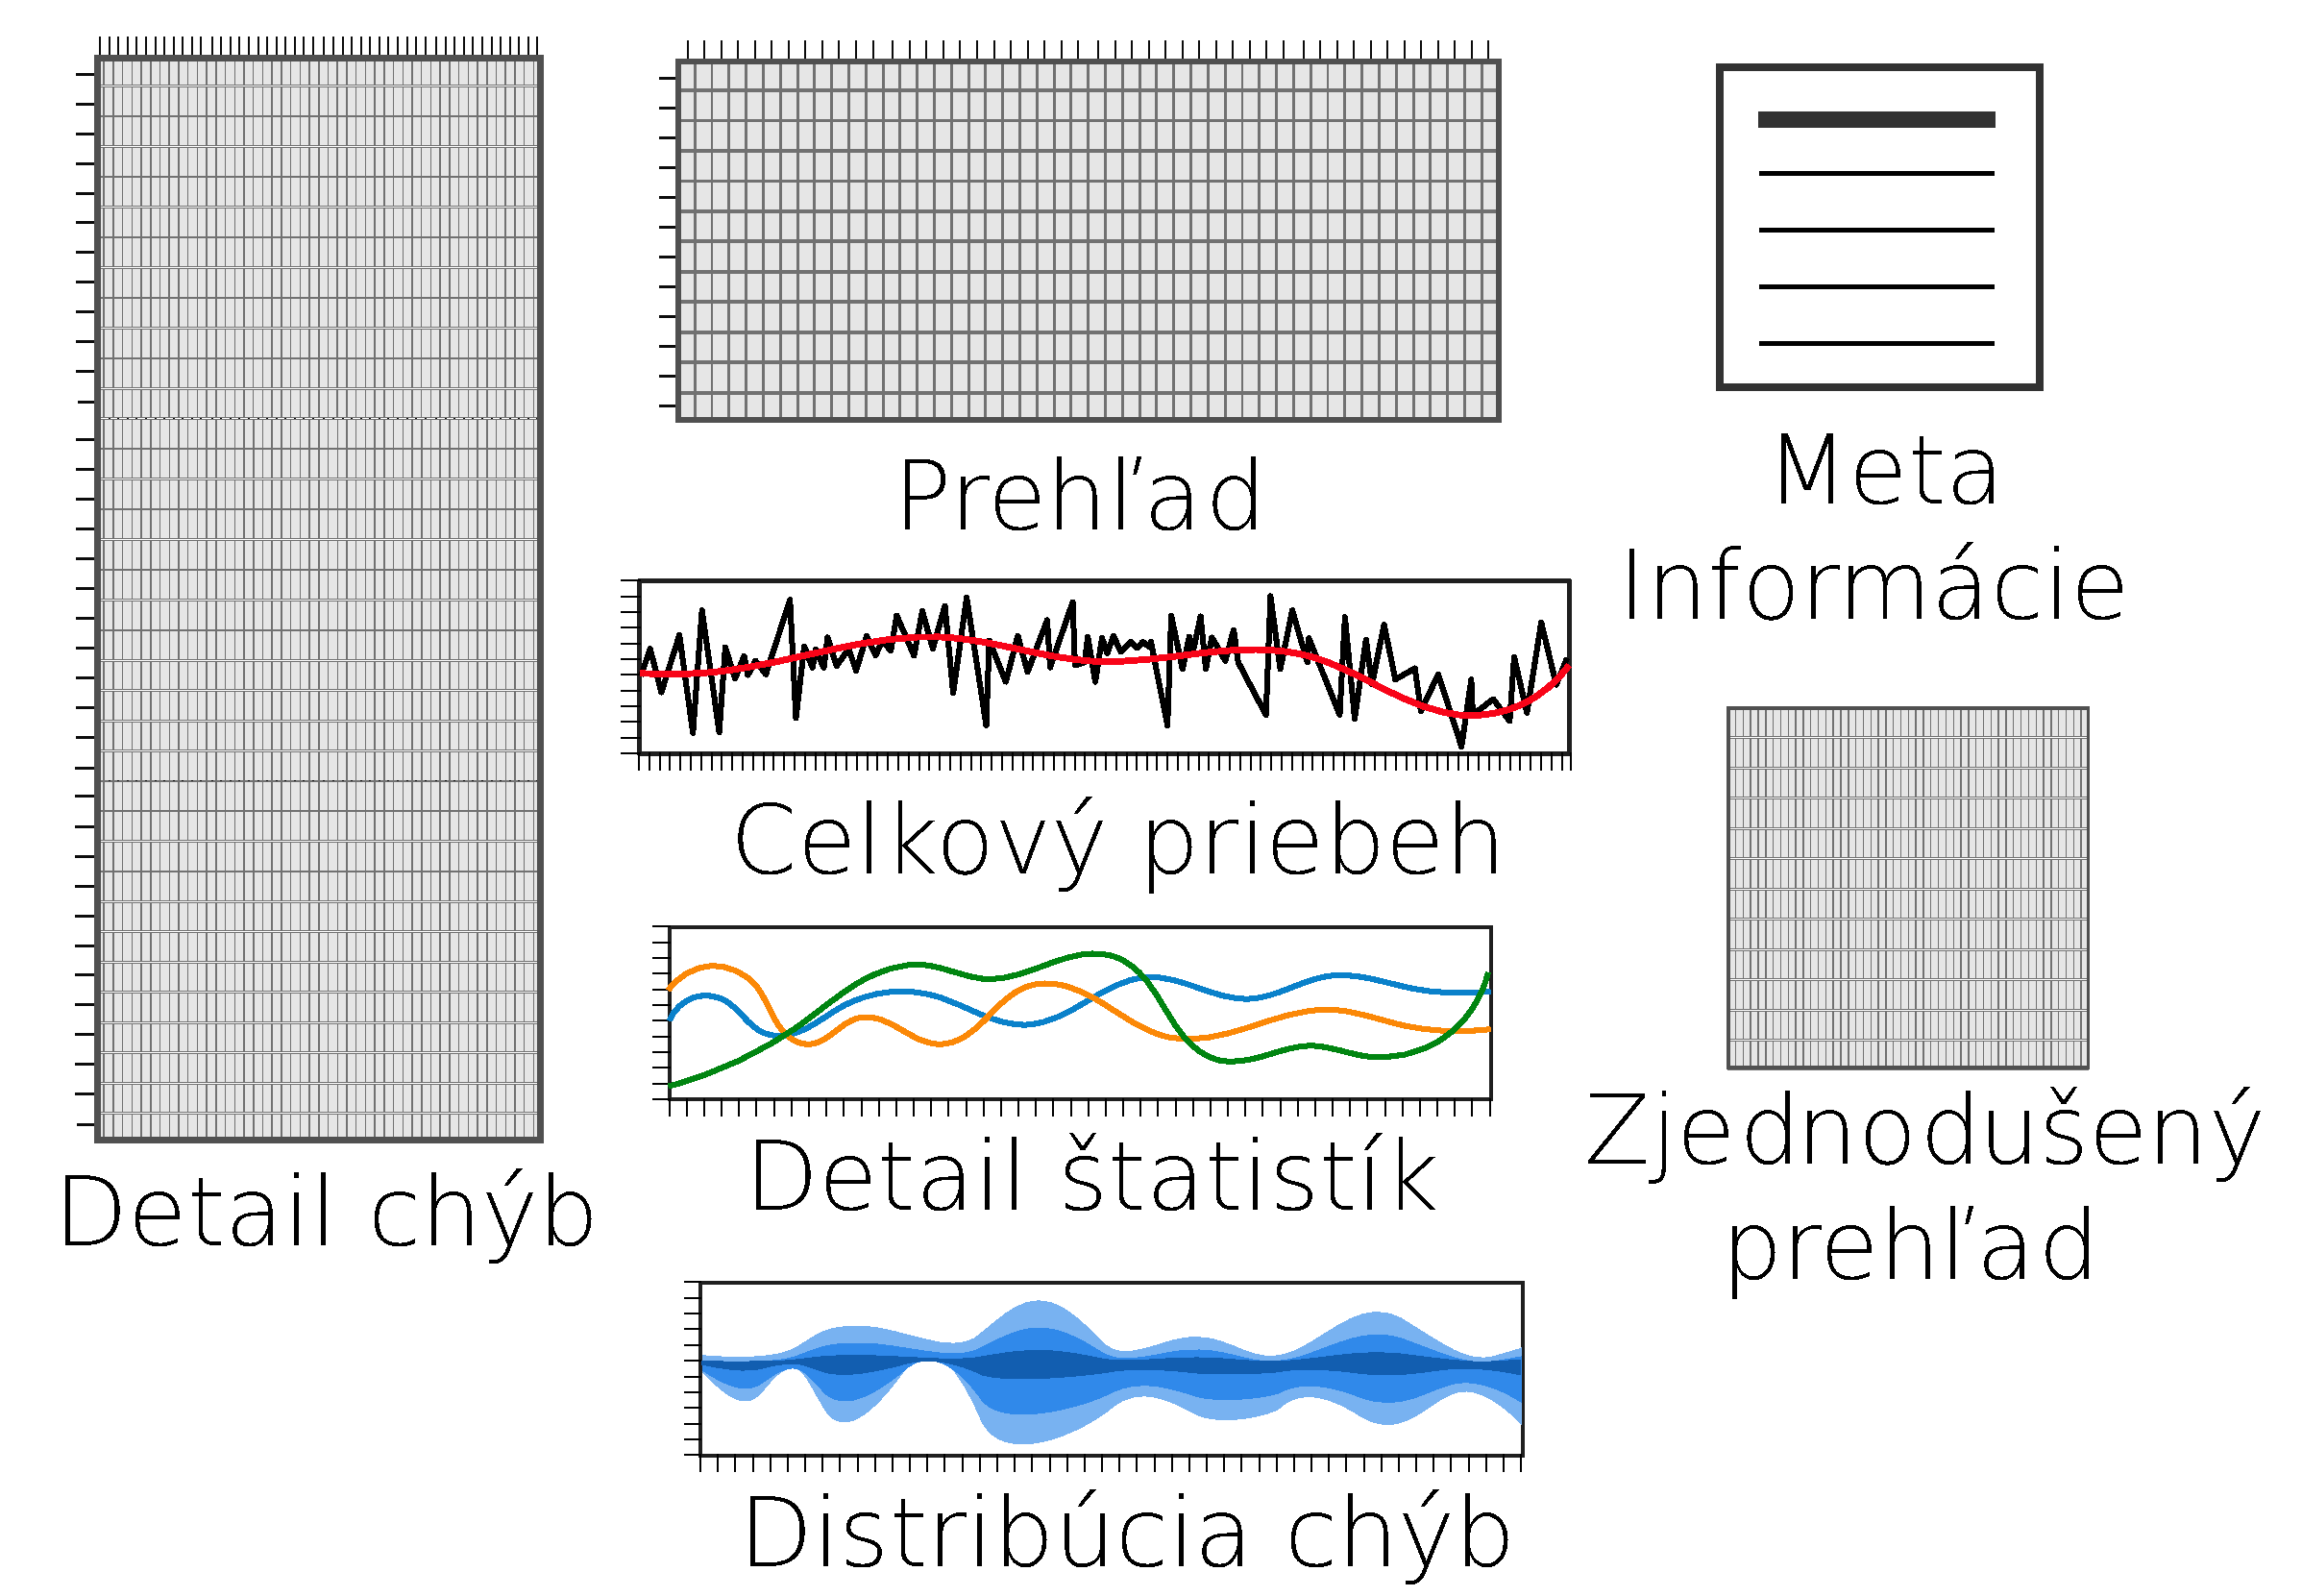
\includegraphics[width = 4.5in]{designicons}
	\caption{Ikony pre jednotlivé prvky vizualizácie}
	\label{fig:designicons}
\end{figure}


\subsection{Viacúrovňový návrh rozloženia prvkov}
Jeden zo spôsobov uvažovania, ako rozložiť prvky vizualizácie, bolo zobraziť ich v jednotlivých úrovniach detailu: 
\begin{easylist}
	# \textit{Úroveň rokov}
	# \textit{Úroveň mesiacov}
	# \textit{Úroveň štatistík}
	# \textit{Úroveň chýb} 
\end{easylist}
Každá úroveň sa skladá z jedného alebo viacerých prvkov rovnakého typu. Napríklad \textit{Úroveň rokov} obsahuje iba prvky \textit{Zjednodušený prehľad}, ktorými sa zobrazujú celé roky. Obmedzením, ktoré kladieme na tento návrh, je zobrazenie maximálne dvoch úrovní súčasne. Touto požiadavkou dosiahneme jednak to, že prvky nebudú zbytočne presahovať mimo obrazovku a taktiež sa zachová do istej miery \textit{detail a kontext}. 

Medzi jednotlivými úrovňami je možný pohyb pomocou klikaním myši na jednotlivé prvky. Napríklad úrovni rokov kliknutím na jeden rok (prvok \textit{Zjednodušený prehľad}) sa nám zobrazí ďalšia úroveň ako prvok \textit{Prehľad}. Ďalším kliknutím na jeden mesiac v danom prvku sa pre daný mesiac zobrazí úroveň štatistík, ako prvok \textit{Detail štatistík}. Ďalej po kliknutí na jednu zo štatistík sa zobrazí prvok \textit{Distribúcia chýb}, v ktorom máme detailne zobrazené chyby, z ktorých sa nám daná štatistika počítala.

Na obrázku \ref{fig:multilevellayout} máme pomocou ikon z obrázka \ref{fig:designicons} schematicky popísané jednotivé úrovne a pohyb medzi nimi. Môžme si všimnúť, že v schéme nie je vidno prvok \textit{Detail chýb}. Dôvodom je, že sa nám kvôli jeho veľkosti nepodarilo nájsť umiestnenie tohto prvku jednak medzi úrovňami a rovnako aj v rámci úrovne.

\begin{figure}
	\centering
	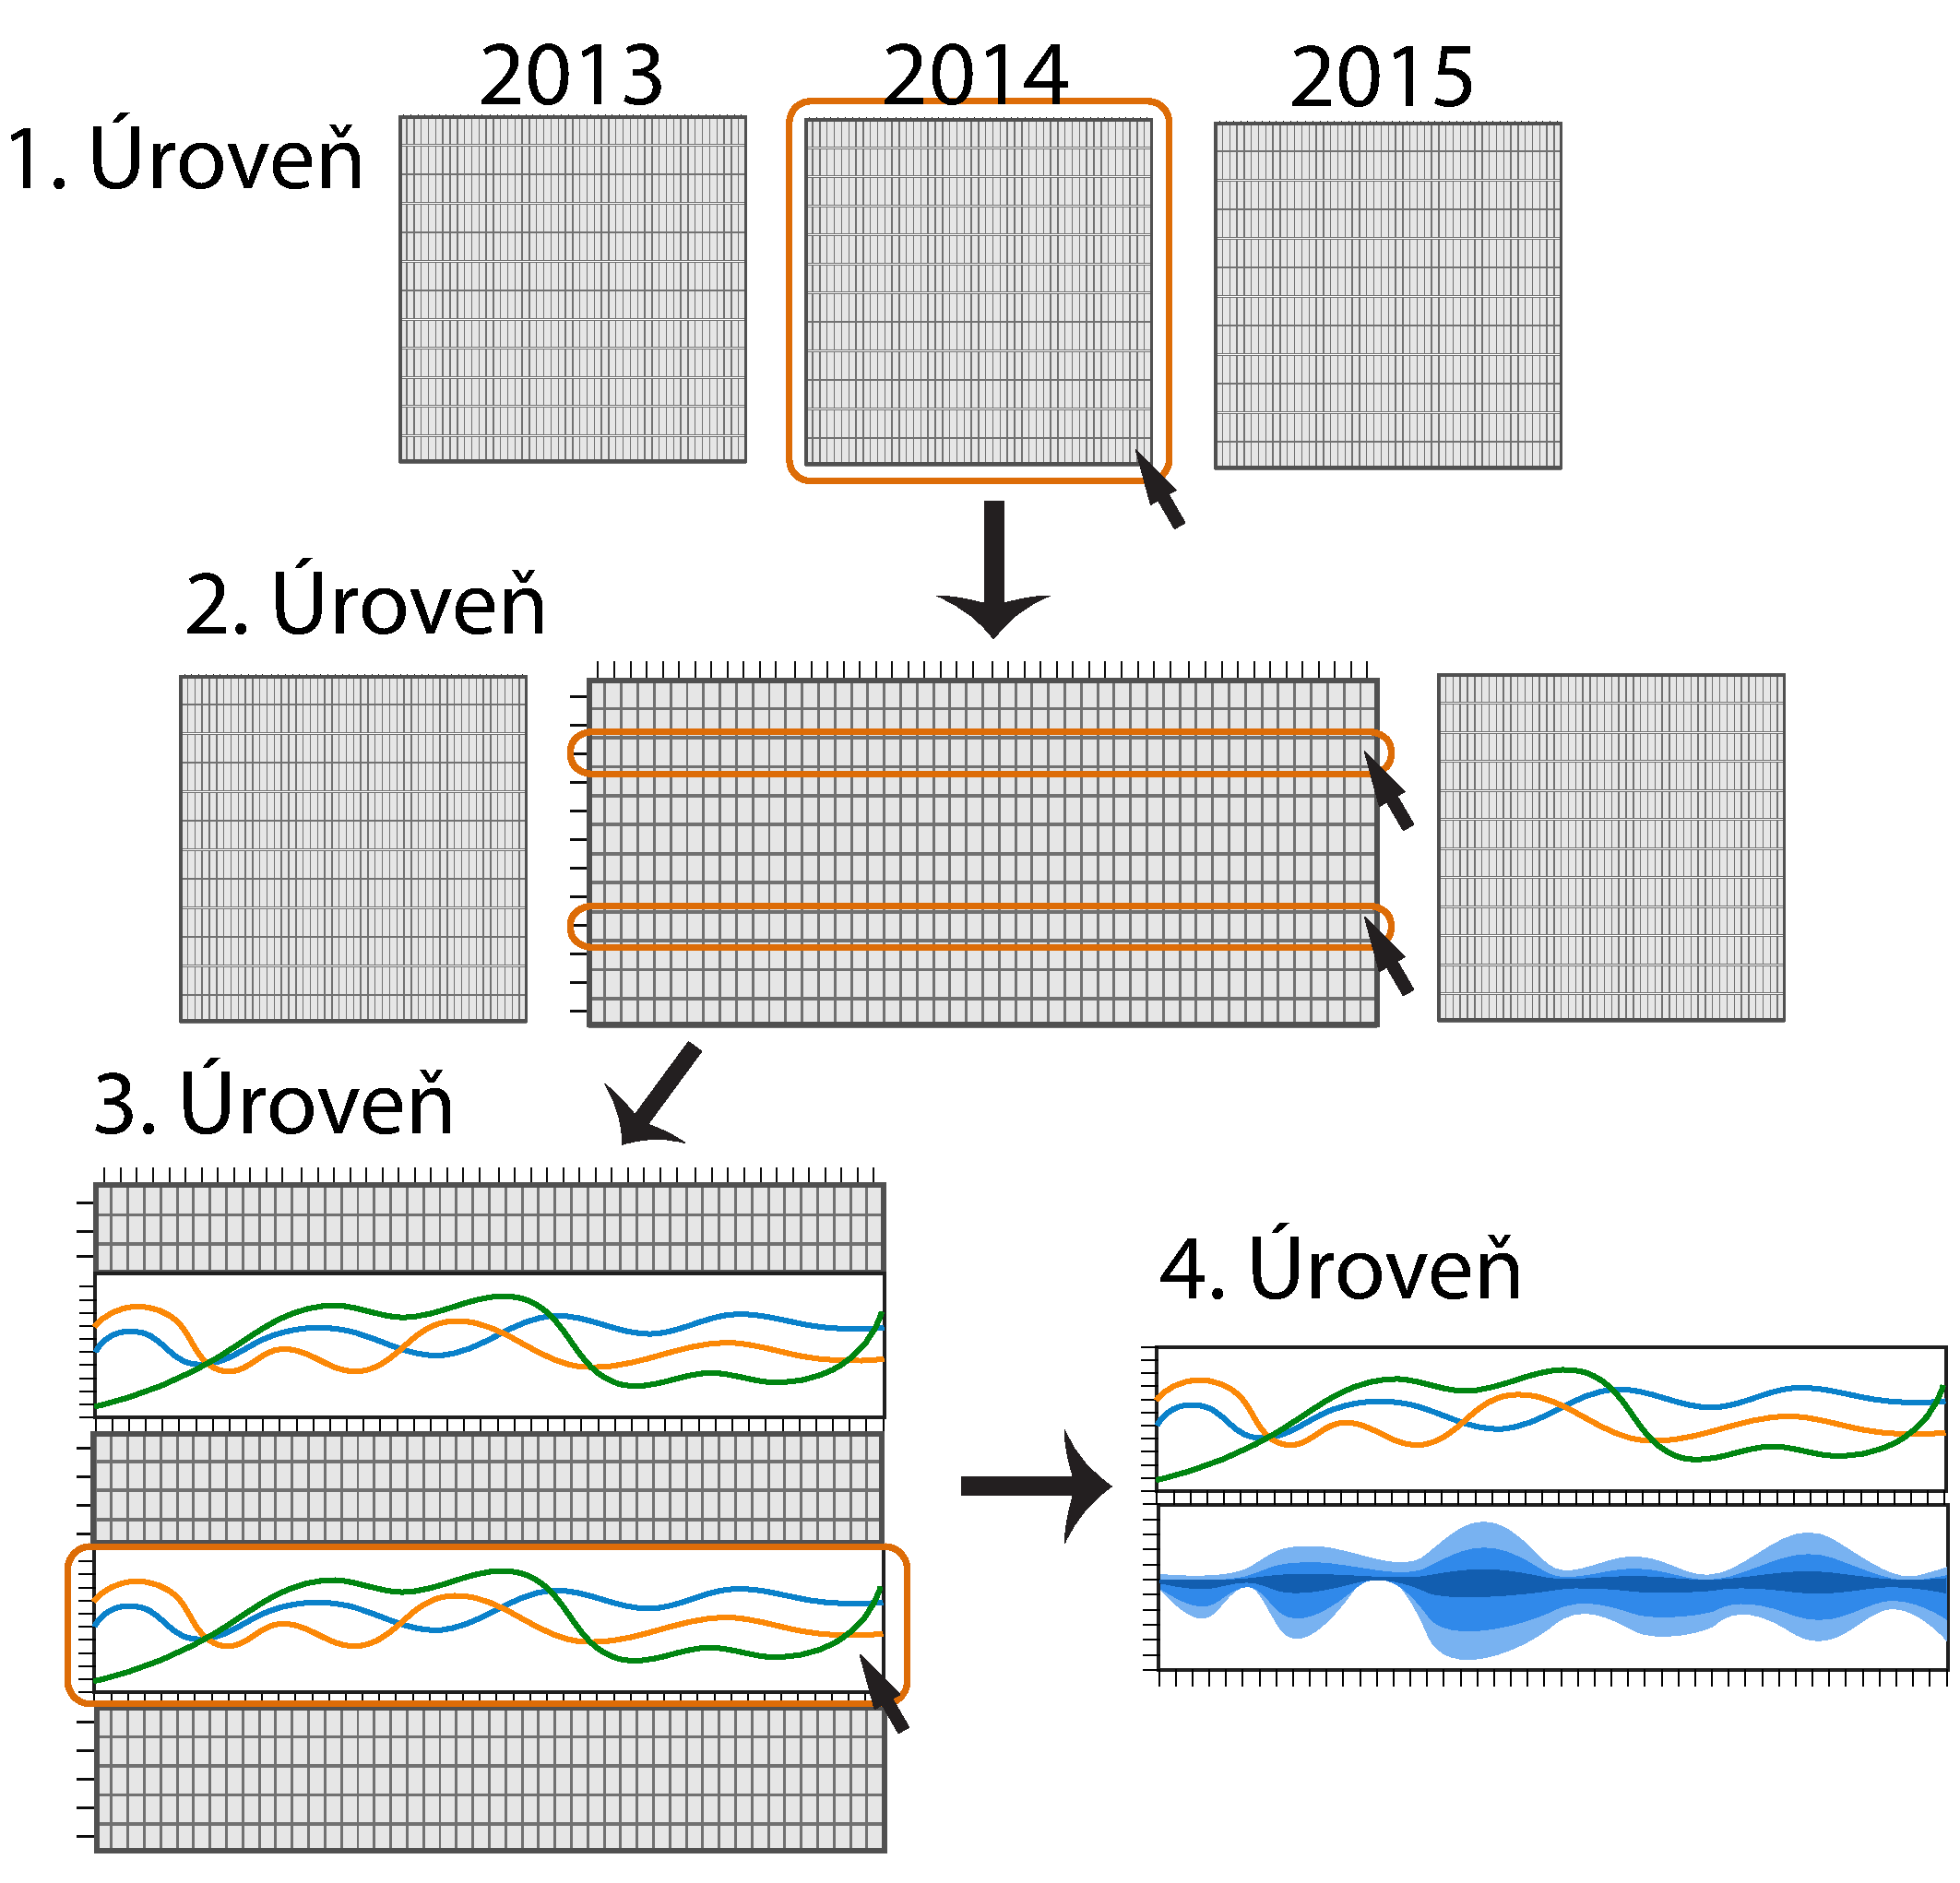
\includegraphics[width = 3.5in]{multilevellayout}
	\caption{Schematické zobrazenie viacúrovňového návrhu rozloženia prvkov vizualizácie}
	\label{fig:multilevellayout}
\end{figure}


\subsection{Plochý návrh rozloženia prvkov}
Pre užívateľa nie je príjemné, keď sa na obrazovke prvky zväčšujú, zmenšujú, posúvajú, objavujú alebo miznú, pretože ... %TODO stráca prehľad alebo čo :D
Preto sme navrhli iný spôsob rozloženia, ktorý tento problém rieši tak, že zobrazí všetky prvky súčasne na jednej úrovni, a teda pojem \textit{úroveň} už nie je potrebný. Spôsob, akým sme umiestnili jednotlivé prvky je schematicky znázornený na obrázku \ref{fig:flatlayout}. Ak potrebujeme vidieť detailnejšie informácie o výkone modelu v mesiaci, tak kliknutím na konkrétny mesiac v prvku \textit{Prehľad}, sa zobrazí \textit{Detail štatistík}, \textit{Distribúcia chýb}, \textit{Detail chýb} pre daný mesiac.

Nevýhodou tohto návrhu je, že nemožno zobraziť viacero prvkov jedného typu súčasne. Z tohto dôvodu nie je možné porovnávať viacero rokov súčasne a preto nie je potrebný komponent \textit{Zjednodušený prehľad}. Zvyšné potrebné porovnávania pre mesiace a distribúciu zaobstará v zníženom, ale dostatočnom detaile, prvok \textit{Prehľad}. 

\begin{figure}
	\centering
	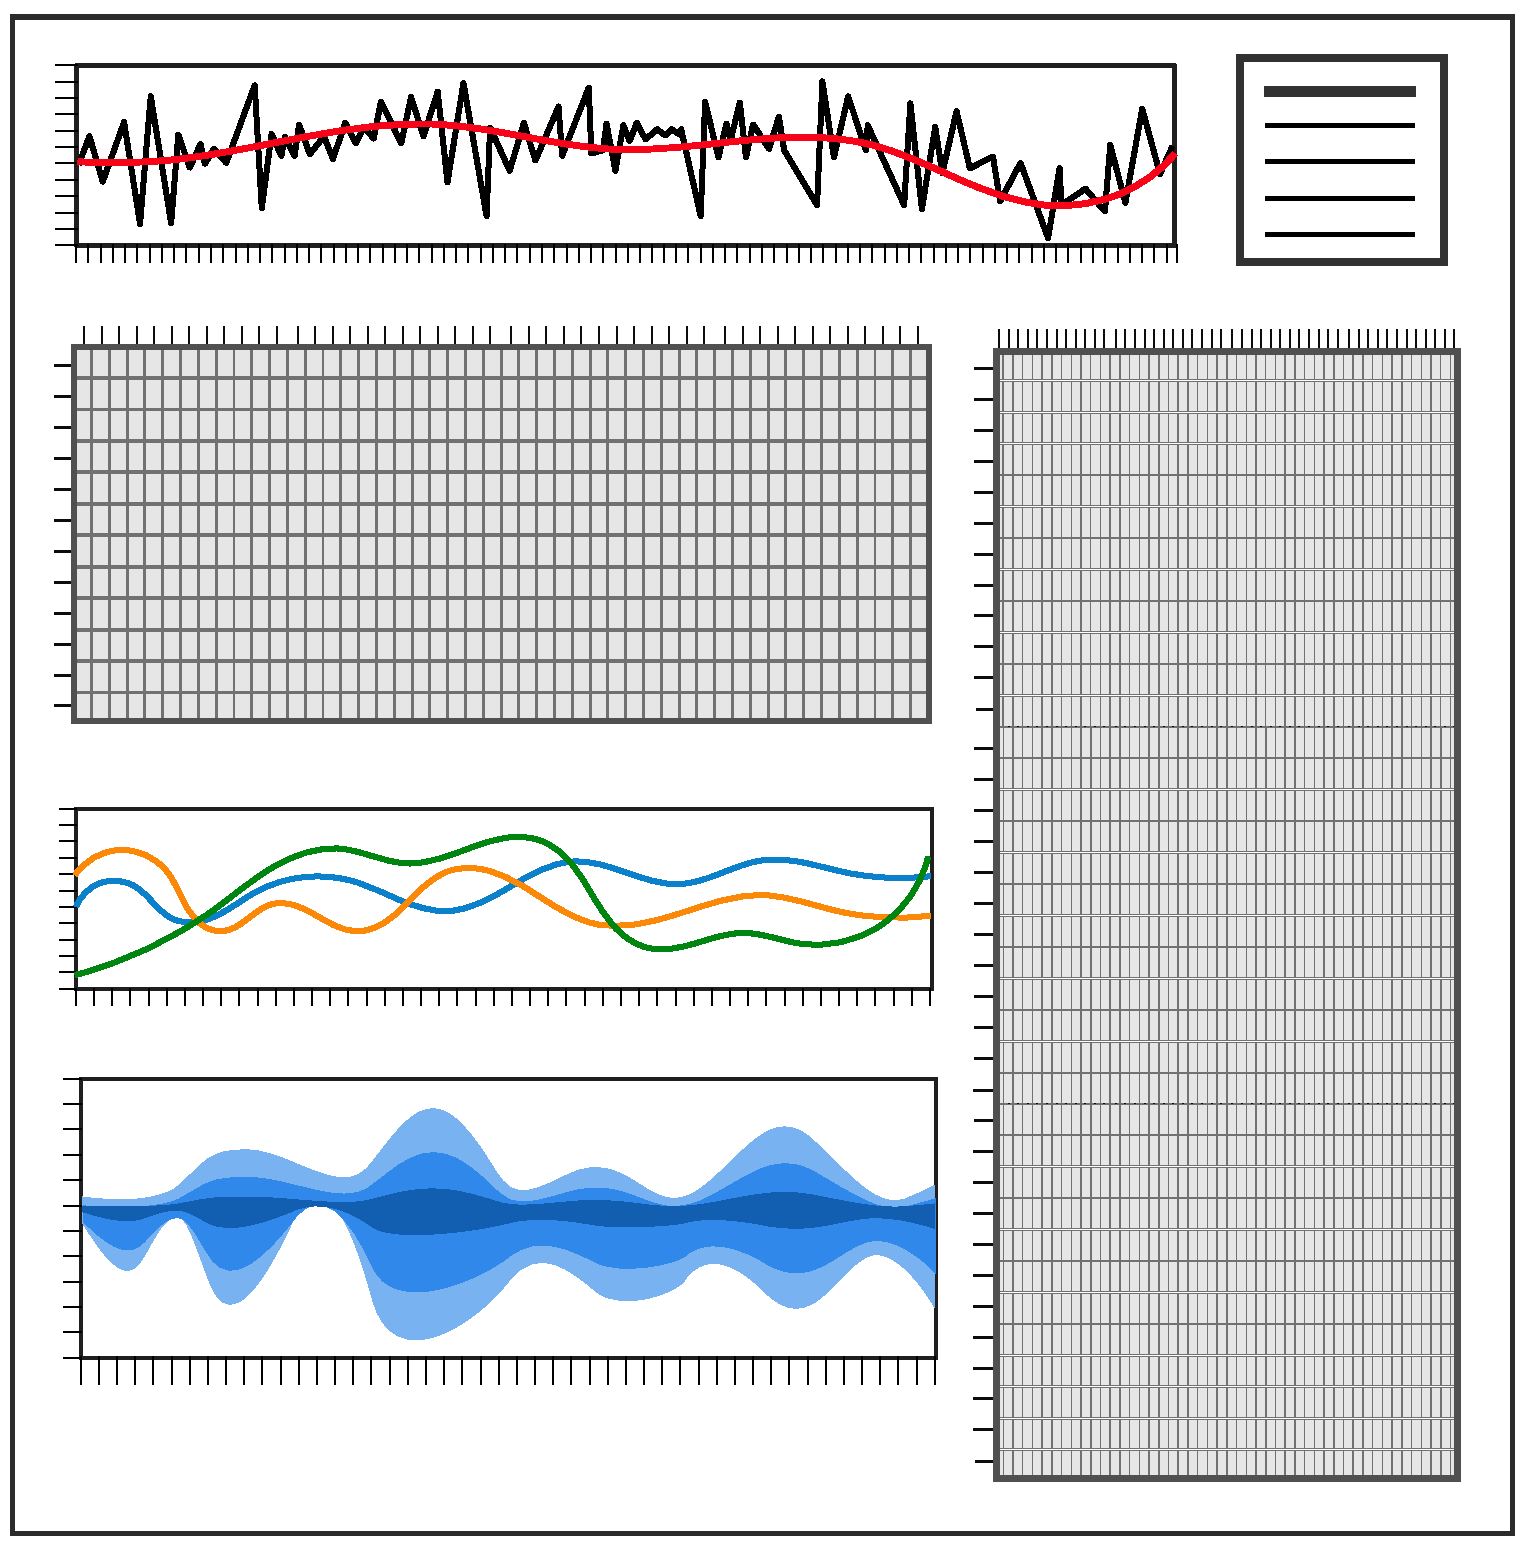
\includegraphics[width = 3.0in]{flatlayout}
	\caption{Schematické zobrazenie plochého návrhu rozloženia prvkov vizualizácie}
	\label{fig:flatlayout}
\end{figure}

\chapter{Návrh systému a Implementácia}
Pri návrhu a implementácii našej aplikácie sme brali do úvahy výhody a obmedzenia systému \textit{IMS4} (\textit{Integrated Monitoring System}), ktorý je vyvíjaný spoločnosťou \textit{MicroStep-MIS s.r.o.}. Dôvodom je, že náš verifikačný systém bol navrhovaný ako prídavný modul pre IMS4.

V tejto kapitole stručne zhrnieme návrh systému a opíšeme kľúčové časti implementácie.


\section{Návrh systému}
\label{sec:sysdesign}
Našu aplikáciu sme sa snažili navrhnúť jednak ako samostatný produkt schopný extrakcie a spracovania meteorologických dát a výpočtu verifikačných štatistík, ale taktiež aj ako súčasť systému IMS4. Toto sme dosiahli tak, že sme rozdelili systém na 2 balíky: \textit{verifikačný} a \textit{vizualizačný}. Na obrázku \ref{fig:system} môžme vidieť schematický návrh systému.

\textit{Verifikačný balík} tvorí jadro celého systému a zohráva viacero úloh. V prvom rade je jeho úlohou extrakcia dát z rôznych dátových zdrojov do tabuliek predpovedí a pozorovaní. Tieto tabuľky sa následne predspracúvajú (párovanie, konverzia fyzikálnych jednotiek, filtrovanie, identifikácia chýbajúcich dát...) a posúvajú sa do časti na výpočet štatistík. Na základe konfigurácie sa spočítajú rôzne štatistiky, ktorých výsledok je výstup z tohoto balíka.

\textit{Vizualizačný balík} chápeme ako vymeniteľnú časť systému. Vďaka tomuto môže byť vizualizácia v podobe interaktívnej obrazovky, ktorá je súčasťou systému IMS4, ale taktiež generovaná automaticky do statických obrázkov na disku.

\begin{figure}
	\centering
	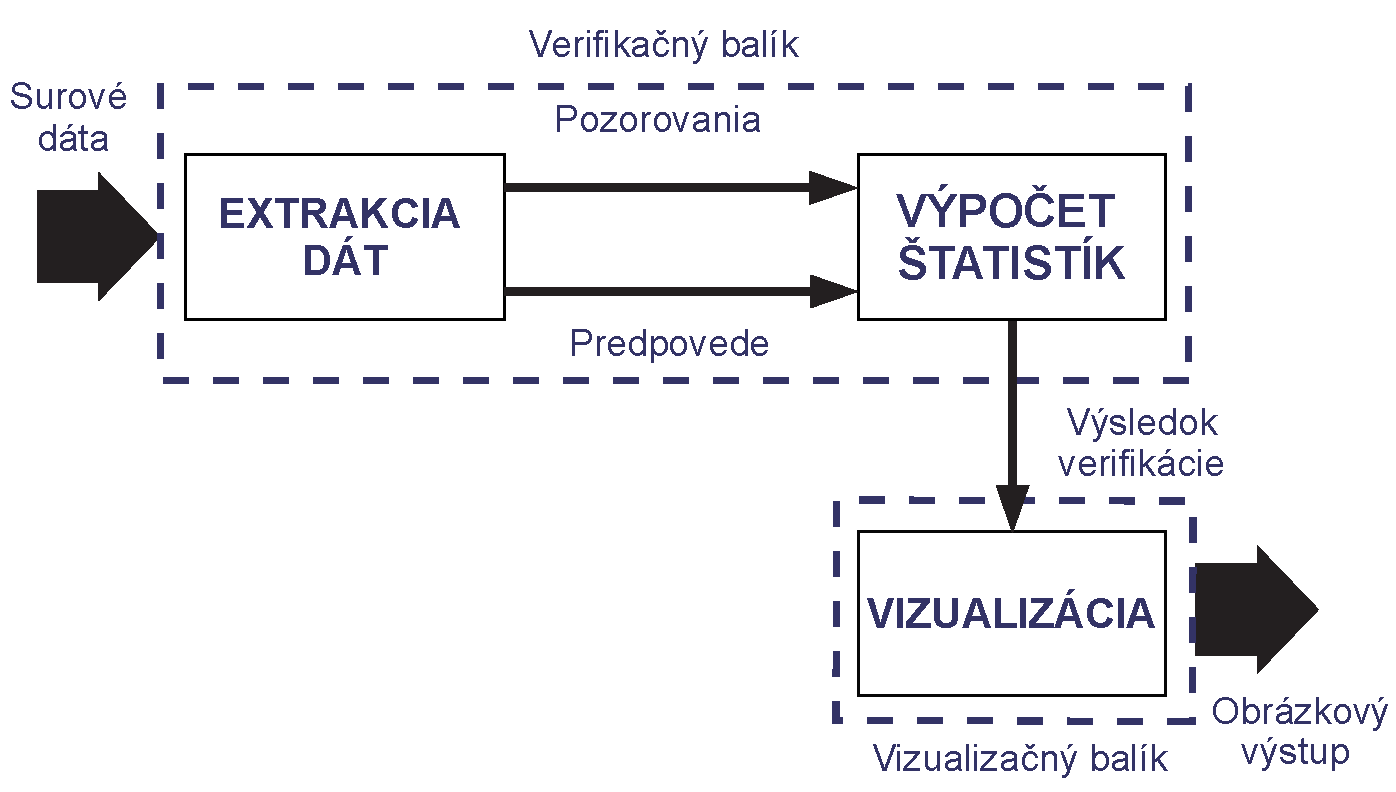
\includegraphics[width = 5in]{system}
	\caption{Schematický popis systému.}
	\label{fig:system} 
\end{figure}

Ak by sme mali systém opísať v pojmoch vizualizácie informácií, tak tieto dva balíky rozdeľujú vizualizačnú \textit{pipeline} na dve časti (Pozri obrázok \ref{fig:pipeline}). Verifikačný balík sa stará o analýzu dát pomocou predspracovania a matematického modelu verifikačných štatistík a taktiež sa stará o filtrovanie dát. Zvyčajne filtrovanie prebieha na základe interakcie užívateľa. V našom prípade sme však uvažovali aj o možnosti, že vizualizácia nebude interaktívna, preto sme filtrovanie umiestnili do verifikačného balíka a vykonáva sa na základe konfigurácie systému. 

Filtrované dáta putujú do vizualizačného balíka. V ňom sa vykonáva zobrazenie hodnôt na vizuálne parametre jednotlivých prvkov vizualizácie, tak ako sme to opísali v kapitole \ref{chap:design} \textit{Návrh vizualizácie}. Takéto dáta sa následne vykreslia do obrázka alebo na obrazovku, čím sa ukončí vizualizačná pipeline.

\begin{figure}
	\centering
	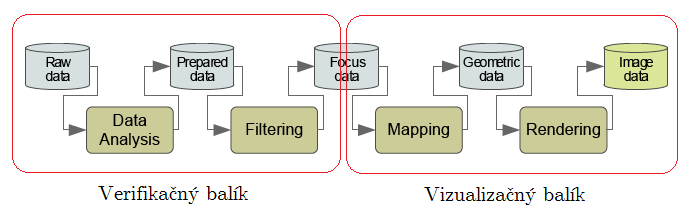
\includegraphics[width = 6in]{pipeline}
	\caption{Rozdelenie prvkov vizualizačnej pipeline do verifikačného a vizualizačného balíka. Obrázok pipeline pochádza zo stránky \protect\url{http://www.infovis-wiki.net}.}
	\label{fig:pipeline} 
\end{figure}

\section{Použité technológie}
Výber implementačných nástrojov bol podmienený obmedzeniami systému IMS4. Z tohto dôvodu sa návrh jednotlivých častí odvíja čiastočne aj od použitej technológie. Aj preto uvádzame v našej práci sekciu \textit{Použité technológie} skôr, ako samotný návrh jednotlivých balíkov.

\subsection{Java}
Primárnu časť systému - \textit{verifikačný balík} sme implementovali v jazyku \textit{Java}, konkrétne vo verzii 1.5. Toto je prvé obmedzenie, ktoré na nás kladie systém IMS4, keďže použitie vyššej verzie (momentálne je dostupná už verzia 1.8) by spôsoboval problém s kompatibilitou.

Java ako programovací jazyk je veľmi rozšírený a obľúbený, vďaka čomu je dostupných pomerne veľké množstvo knižníc, nevynímajúc originálne knižnice zahrnuté v systéme IMS4. Tieto knižnice sme využili pri implementácii aj my. Môžme spomenúť 3 knižnice, z ktorých sú dve interné a jedna pôvodne externá s pridanou funkcionalitou. Prvé dve spomenuté sú \textit{Log} - používaná na logovanie a \textit{X2O}, ktorá sa používa na mapovanie javovských objektov na XML štruktúru a späť pomocou \textit{Java Reflection API}. My sme X2O použili pri ukladaní a načítavaní konfiguračných súborov. Posledná knižnica je NetCDF-grib \cite{XYZ} a pochádza od americkej organizácie \textit{Unidata}, ktorú zastrešuje \textit{UCAR}. Jedná sa o opensource produkt na čítanie dát zo súborov vo formáte GRIB. My využívame upravenú verziu NetCDF-grib-6.0 obzvlášť kvôli Jave 1.5, aj keď sú dostupné novšie verzie \footnote{Najnovšia je NetCDF-Java-4.5, ktorá zoskupuje všetky ďalšie podobné produkty od Unidata.}.

\subsection{JavaScript}
Systém IMS4 využíva webové stránky na vytváranie GUI. Z tohto dôvodu sme sa rozhodli, že vizualizáciu budeme produkovať priamo v prehliadači pomocou \textit{JavaScriptu}. Podobne ako Java, aj JavaScript je veľmi populárny a preto vzniklo veľké množstvo rôznych knižníc, medzi ktorými sú aj mnohé určené na vizualizáciu. Medzi najznámejšie z nich patria napríklad: \textit{JavaScript InfoVis Toolkit}, \textit{Highcharts}, \textit{jQuery Visualize}, \textit{JS Charts}, \textit{jqPlot}, \textit{jpGraph}, \textit{Raphaël}, \textit{Dygraphs},\textit{ Processing.js}, \textit{Axiis}, \textit{D3} a mnohé ďalšie. Pre naše účely sme z veľkého množstva knižníc vybrali práve D3, ako najvhodnejší nástroj na náš účel.

\subsubsection{D3}
D3 (\textit{Data-Driven Documents}) \cite{XYZ} je opensource knižnica napísaná v JavaScripte. Na vizualizáciu využíva HTML a SVG elementy a ich vizuálne vlastnosti, ktoré mení pomocou ich atribútov a CSS štýlov. 

Dôvodom, prečo sme si vybrali práve D3 z veľkého množstva vizualizačných knižníc je, že väčšina z nich bola zameraná na konkrétny druh vizualizácie (napr. \textit{force-directed layout}) alebo na niekoľko najpoužívanejších druhov diagramov (bodový, stĺpcový, čiarový, histogram,...). D3 sa však nezameriava na konkrétny druh vizualizácie, ale ponúka spôsob, ako zobrazovať hodnoty na vizuálne parametre elementov, čím umožňuje ohromnú variabilitu a je vhodná na vytváranie nových alebo menej používaných typov vizualizácií. Väčšina vizualizácií, ktoré sme v našej práci sme navrhli, nie sú podporované vyššie spomenutými knižnicami a preto sme potrebovali nástroj umožňujúci dobre parametrizovateľnú vizualizáciu.

Toto je taktiež dôvod, prečo vzniklo veľké množstvo knižníc, ukážkových príkladov a návodov ktoré využívajú práve D3. Aby sme spomenuli aspoň niektoré z knižníc používajúcich D3, tak sú to napríklad \textit{Raw}, \textit{Cubism}, \textit{Ember Charts}, \textit{NVD3}, \textit{C3}, \textit{MetricsGraphics}, \textit{Graffeine}, \textit{Mermaid}, \textit{Epoch}, \textit{Insights}, \textit{Dashku}, \textit{RickShaw} a mnohé ďalšie. 

\section{Verifikačný balík}
Ako sme už spomenuli v sekcii \ref{sec:sysdesign} , tento balík sa skladá z dvoch logických častí \textit{Spracovanie dát} a \textit{Výpočet štatistík}. V tejto sekcii sa pokúsime zhrnúť kľúčové prvky návrhu a implementácie týchto dvoch častí.
\subsection{Spracovanie dát}
Úlohou tejto časti je získanie potrebných dát z určených dátových zdrojov a ich predspracovanie tak, aby mohli vstúpiť do ďalšej časti - \textit{Výpoečt štatistík}.

Pri návrhu tried na získavanie predpovedí a pozorovaní sme sa snažili, aby bolo užívateľovi umožnené získavať dáta z viacerých typov zdrojov: Gribovské súbory, CSV súbory, webové zdroje, databáza a podobne. Aby sme pre každý typ zdroju nevytvárali samostatnú vetvu udalostí, navrhli sme abstraktnú triedu \textit{DataExtractor}, ktorá obsahuje abstraktné metódy \texttt{extract()} a \texttt{addSoruces()} a taktiež slúži na inštancovanie všetkých jej potomkov (pozri UML diagram na obrázku \ref{fig:dataextractor}). Jednotlivý potomkovia následne musia implementovať vyššie spomenuté metódy, ktoré sú špecifické pre každý typ zdroju.

Z extrakcie dát získame tabuľky hodnôt s pozorovaniami a predpoveďami pre konkrétne časy. Tieto dáta sa následné predspracúvajú v štyroch krokoch:

\begin{enumerate}
	\item \textit{Párovanie} : Prebieha tak ako je opísané v podsekcii \ref{subsec:pairing}.
	\item \textit{Filtrovanie} : Na základe konfigurácie získavame iba dátumy zvolené užívateľom.	\item \textit{Konverzia jednotiek} : Fyzikálne jednotky z predpovedí a pozorovaní konvertujeme do rovnakej jednotky podľa konfigurácie, aby bol výpočet chýb korektný.
	\item \textit{Výpočet chýb} : Prebieha tak ako je opísané v sekcii \ref{sec:errormeasurement}.
\end{enumerate}

\noindent Tak ako je naznačené na obrázku \ref{fig:system},  takto spracované dáta putujú do časti výpočet štatistík.

\begin{figure}
	\centering
	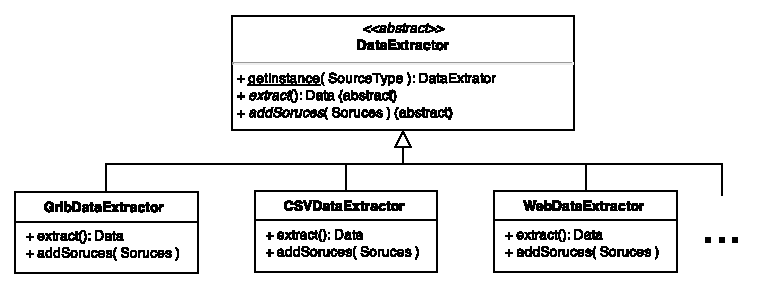
\includegraphics[width = 5.5in]{dataextractor}
	\caption{Triedny UML diagram pre triedy typu DataExtractor.}
	\label{fig:dataextractor} 
\end{figure}

\subsection{Výpočet štatistík}
V tejto časti verifikačného balíka sa vykonáva výpočet štatistík, z ktorých sme väčšinu opísali v sekcii \ref{sec:errormeasurement}. 

Pri implementácii sme využili nami navrhnutý všeobecný spôsob výpočtu kumulovanej chyby (pozri podsekciu \ref{subsec:cumulativeerror}). Pripomenieme, že sme v našom využili vzorci dve funkcie $ \Phi $ a $ \varepsilon $, ktoré obe boli ľubovoľnými funkciami z $\mathbb{R}$ do $\mathbb{R}$. Na obrázku \ref{fig:stats} je triedny diagram tried slúžiacich na výpočet spojitých štatistík verifikácie. V Diagrame môžme vidieť abstraktnú triedu \textit{ContinuousStatistics}, ktorá reprezentuje ľubovoľnú štatistickú metódu na výpočet kumulovanej chyby opísanú v sekcii \ref{sec:errormeasurement}. Táto trieda obsahuje metódu \texttt{calculateStatistics()}, ktorá vypočítava ľubovoľnú kumulovanú chybu s použitím dvoch abstraktných metód: \texttt{processError()} a \texttt{processSum()}. Tieto dve metódy predstavujú funkcie $ \Phi $ a $ \varepsilon $. Ako vidíme na obrázku všetky štatistické sú implementované ako potomkovia triedy \textit{ContinuousStatistics} a implementujú tieto vyššie spomenuté metódy. 

%TODO\pagebreak
             

\begin{figure}
	\centering
	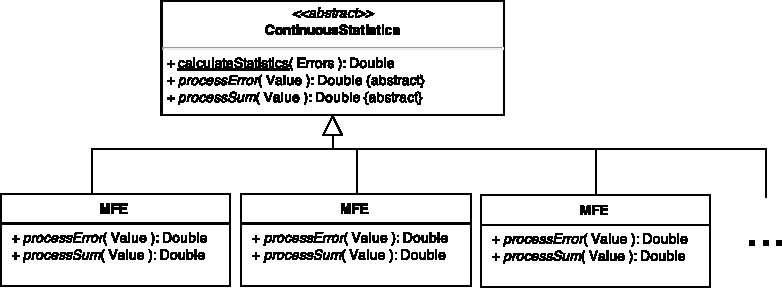
\includegraphics[width = 5in]{stats}
	\caption{Triedny UML diagram pre triedy typu ContinuousStatistics.}
	\label{fig:stats} 
\end{figure}

\section{Vizualizačný balík}
Úlohou vizualizačného balíka je spracovávať výsledky verifikácie a vytvoriť z týchto dát obrazovku vizualizácie navrhnutú v predošlej kapitole. 

Pri návrhu a implementácii tohto balíka sme sa snažili využiť niektoré vlastnosti, ktoré nám ponúkajú použité technológie. Veľkú časť tohto balíka sme navrhli ako súčasť knižnice D3 s vyžitím návrhových vzorov charakteristických pre túto knižnicu. Jednak išlo o takzvaný \textit{chaining pattern}, ktorý slúži pri vytváraní objektu, kedy sa dovoľuje volanie jeho metód, ktorými sa nastavujú jeho vlastnosti, neustále za sebou. Príklad pre lepšie pochopenie je na výpise \ref{list:chaining}.
Ďalším vzorom je \textit{callback pattern}, kedy používame funkciu ako parameter. 


\begin{lstlisting}[frame=solid, backgroundcolor=\color{bg}, basicstyle=\footnotesize\ttfamily, language=JavaScript, numbers=left, numberstyle=\tiny\color{black}, caption=Ukážka aplikácie návrhového vzoru \textit{chainning}., captionpos=b, label=list:chaining]
var groups = group.selectAll(".group")
		    .data(data)
		    .enter()
		    .append("svg:g")
		    .classed("group", true);	
\end{lstlisting}


\chapter{Výsledky}

\chapter*{Záver}
\addcontentsline{toc}{chapter}{Záver}

V našej práci sme uviedli problém verifikácie predpovedných modelov počasia so zameraním na verifikáciu predpovede spojitej premennej v jednom bode. Zhrnuli sme používané štatistické metódy na meranie chyby predpovede a navrhli sme spôsob všeobecného výpočtu kumulovanej chyby, ktorý sme v závere využili aj pri implementácii.

Taktiež sme preskúmali doterajšie riešenia jednak z pohľadu verifikačného softvéru, ale aj z pohľadu vizualizačných techník vo verifikácii. Uviedli sme slabé a silné stránky jednotlivých softvérových riešení a zhrnuli sme ich v prehľadnej tabuľke. Taktiež sme opísali a analyzovali vizualizácie používané vo verifikácii a načrtli ich zameranie a spôsob použitia.

Ďalej sme charakterizovali vstupné dáta a špecifikovali požiadavky používateľov, na základe ktorých sme navrhli rôzne spôsoby vizualizácie, ktoré sme implementovali ako doplnok JavaScriptovej knižnice D3. V závere práce sme následne vykonali testovanie našej vizualizácie na základe čoho sme zhodnotili jej úspešnosť.

Výsledkom práce je teda verifikačný nástroj schopný spracovávať dáta z rôznych zdrojov, ponúkajúc funkcionalitu pre verifikáciu predpovedí spojitej premennej s použitím špeciálne navrhnutej vizualizácie pre tieto účely. 

\subsubsection{Prínos}

Za hlavný prínos tejto práce považujeme práve návrh špecializovanej vizualizácie, ktorá síce nevyniká obrovskou inováciou, ale pri jej vzniku sme navrhli mnoho drobných originálnych vylepšení smerujúcim k lepšiemu, rýchlejšiemu a jednoduchšiemu porozumeniu dát. Príkladom môže byť návrh prehľadovej vizualizácie verifikačných dát, návrh riešenia viacerých škál pri \mbox{mnoho-čiarovom} diagrame, zovšeobecnenie re-dizajnu krabicového diagramu od \mbox{Bada et. al.} \cite{Bade} na takzvaný \textit{Pruhový diagram}, využitie dvojtónového pseudofarbenia pri kompaktnej vizualizácii distribúcie dát pomocou grafu hustoty a podobne.

Medzi prínosy našej práce patrí aj to, že nami vyvinutý systém a si nájde praktické uplatnenie pri riešení skutočných problémov reálneho sveta. Ku príkladu bol tento systém predaný do Singapúru pre Radmon (\textit{Radiation Monitors}), ale využitie si nájde aj

\subsubsection{Budúca práca}

Na výskum a vývoj neustále existuje priestor a v našej práci ho vidíme určite mnoho obzvlášť v štyroch oblastiach:
\begin{enumerate}
	\item \textit{Získavanie dát} - V práci sme implementovali 3 typy zdrojov: Grib, CSV a Web. Avšak existuje mnoho ďalších zdrojov dát, z kade možno získať pozorovania, rovnako ako aj predpovede. Príkladom je napríklad \textit{databáza}, \textit{XML}, alebo \textit{XLS} súbory, takzvané \textit{bloky} systému IMS4, kde sú aj merania a mnohé iné ďalšie zdroje. 
	\item \textit{Konfigurácia systému a vizualizácie} - Konfigurovanie systému v momentálnom stave nie je veľmi user-friendly úloha. V budúcej práci očakávame návrh riešenia, ktoré skryje pred užívateľom pomerne neprehľadné nastavenia systému.
	\item \textit{Interaktívna manipulácia s dátami} - Momentálne riešenie neponúka veľmi dôležitú súčasť moderných vizualizačných nástrojov a tým je manipulácia s dátami priamo na obrazovke. Príkladmi operácií môže byť filtrovanie dát na základe rôznych kľúčov alebo selekcia vybranej vzorky dát pomocou \textit{brushingu} a podobne.
	\item \textit{Porovnávanie modelov a staníc} - Pri návrhu vizualizácie sme nezvažovali možnosť porovnávania výkonu viacerých predpovedných modelov alebo porovnávanie predpovedí pre rôzne stanice súčasne. Riešenie takéhoto problému by pravdepodobne vyžadovalo zásadný re-dizajn vizualizácie.
	\end{enumerate} 	
\appendix
\chapter{Prílohy}

%TODO toto nebude tu, ale cele to dam do demnostracie asi!
\section{GUI}
{ \hspace*{-0.3in}
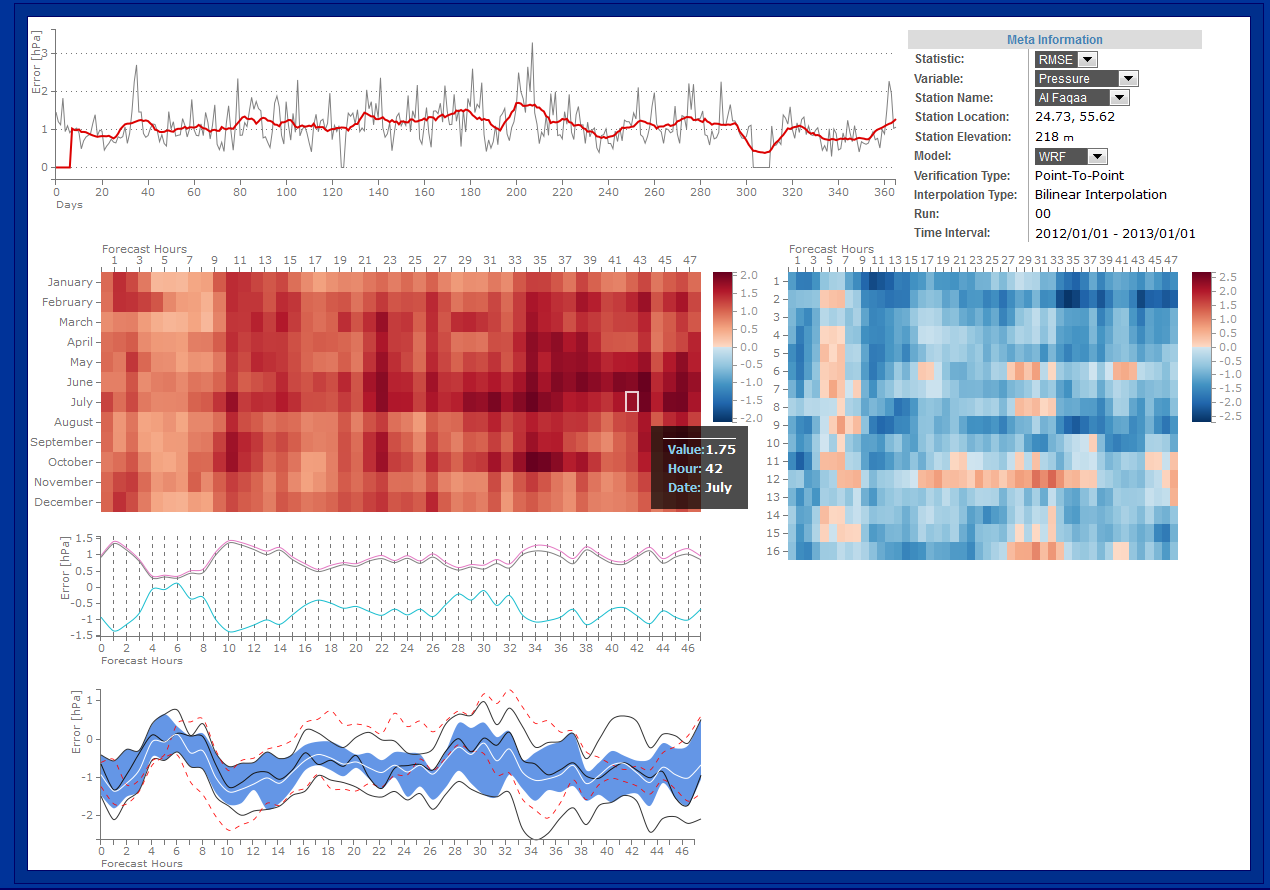
\includegraphics[width=7in]{gui} 
}

\section{Testovací formulár}
\label{sec:testform}
{
\hspace*{-1in}
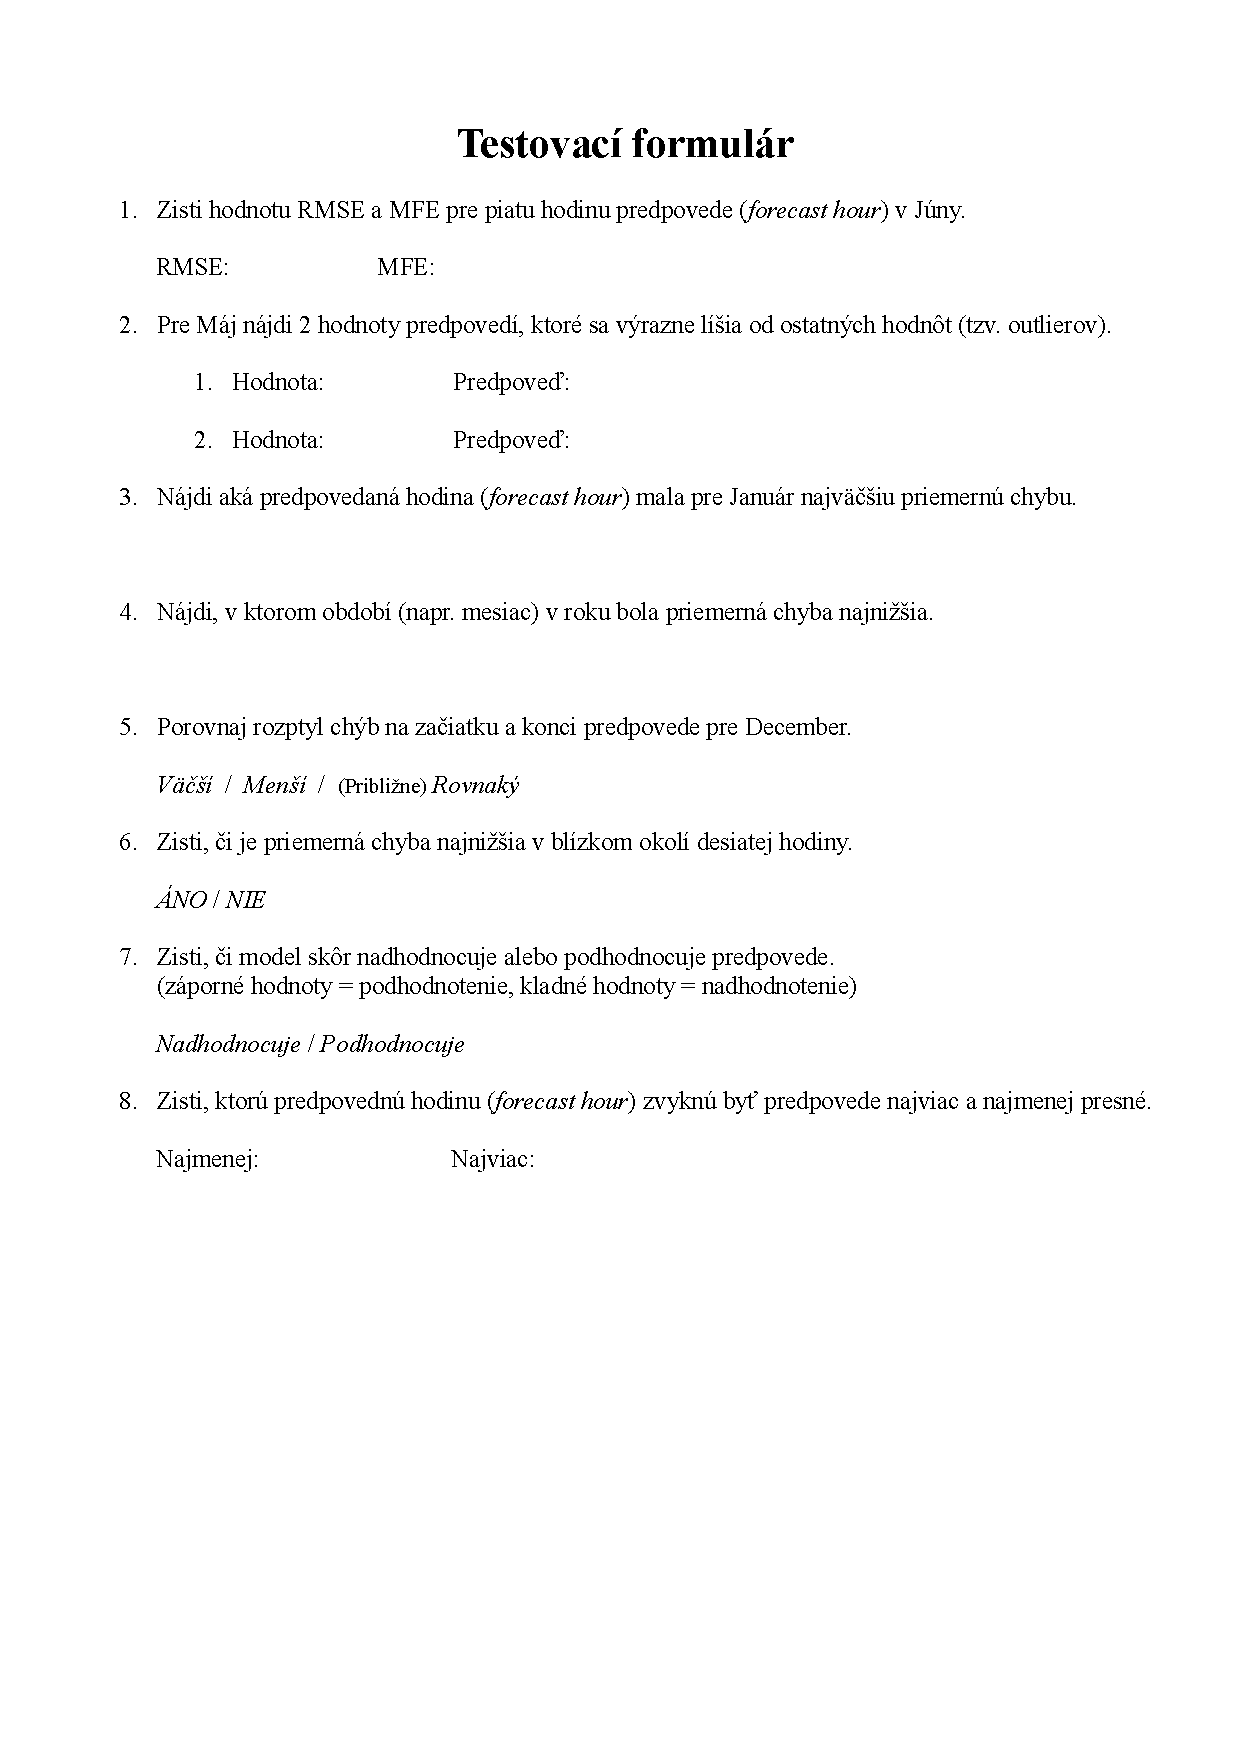
\includegraphics[width=597pt,height=780pt]{testform}
}
% 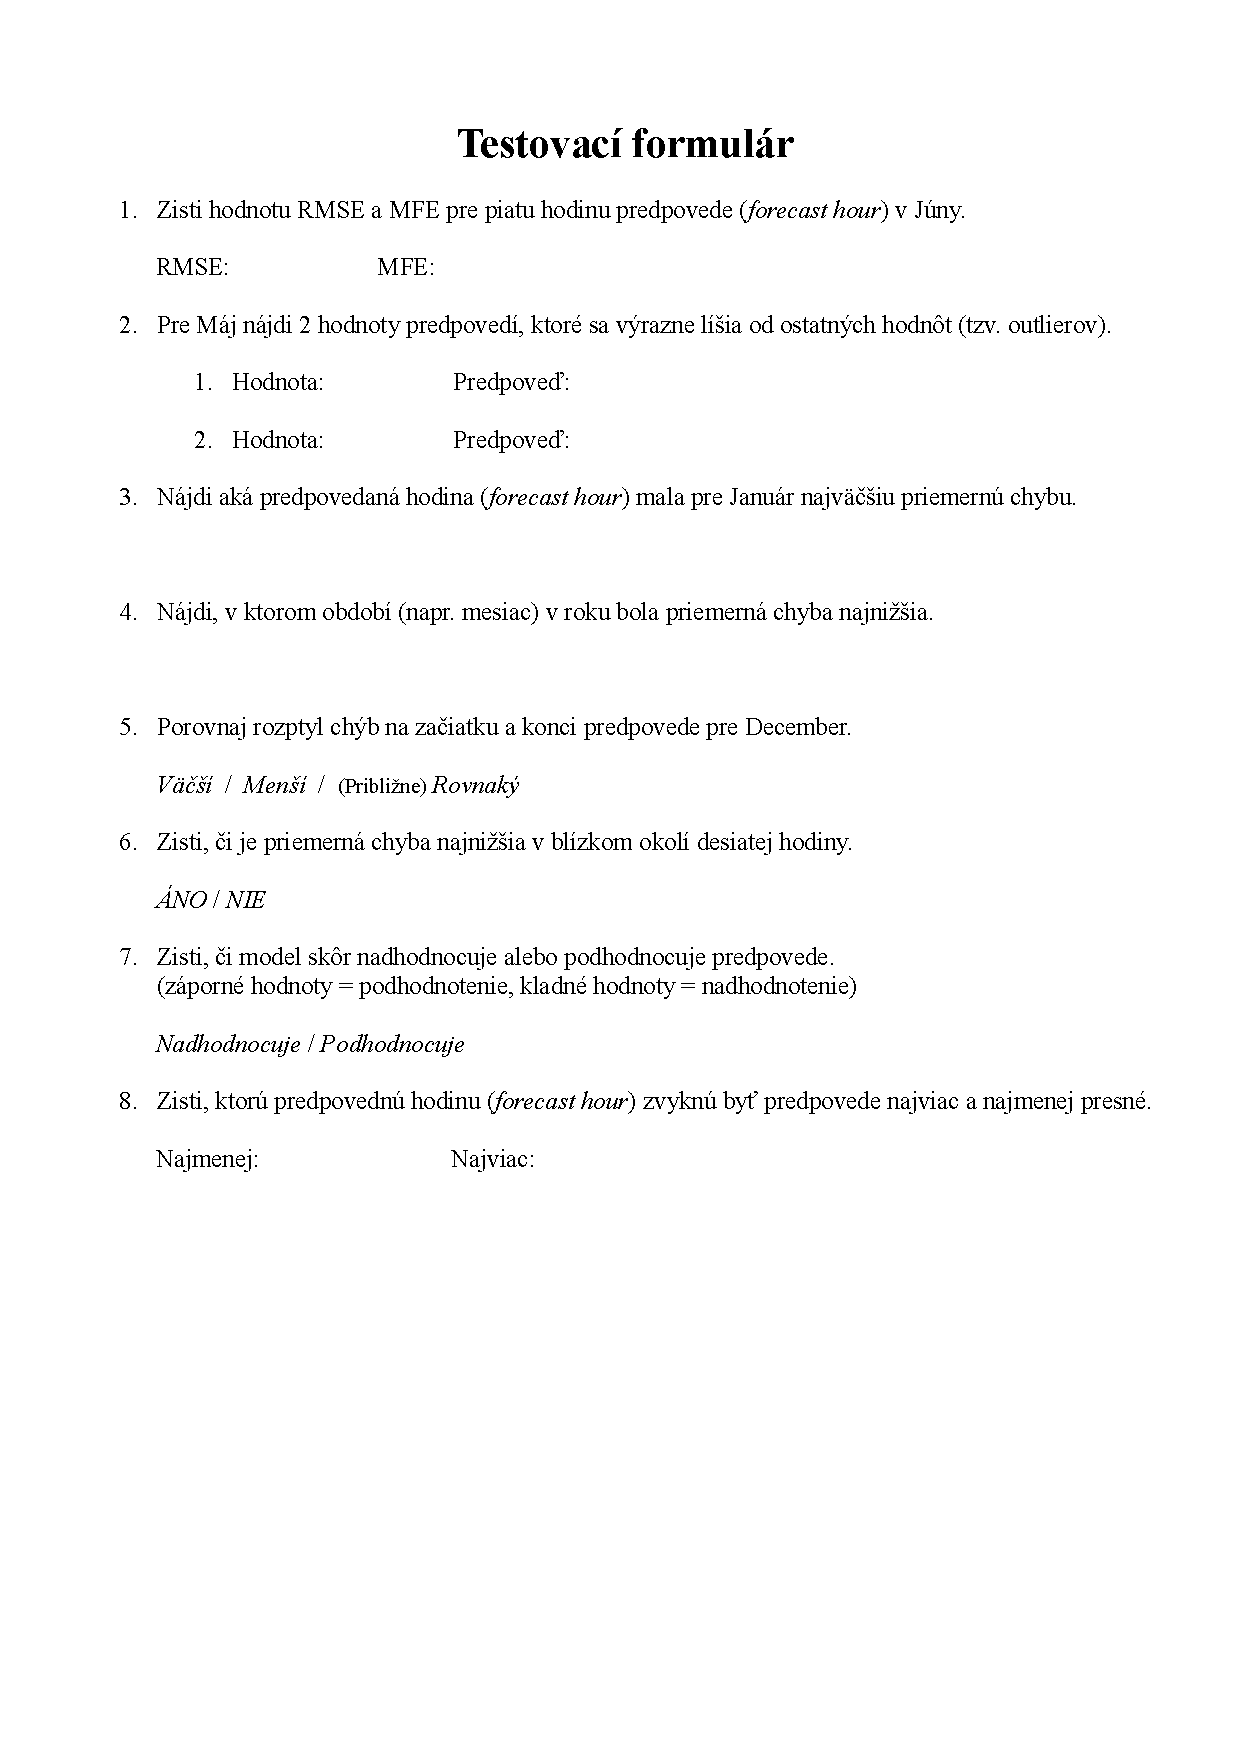
\includepdf[pages={1}]{testform.pdf}


\section{CD}
Obsah CD:
\begin{easylist}[itemize]
	# Zdrojové súbory
	# Testovacie dáta
	# Elektronická verzia práce
\end{easylist}


\bibliographystyle{alpha}
\raggedright
\bibliography{verification,prevSoft,prevVis,design,implementation,results}


\end{document}
